\documentclass{book}

\usepackage{graphicx}
\usepackage{moreverb}
\usepackage{amsmath}
\usepackage{alltt}
\usepackage{rotating}
\usepackage{subfigure}
\usepackage{toc}
\usepackage{xspace}
\usepackage{makeidx}

\usepackage[colorlinks=true]{hyperref}

\newcommand{\sref}[1]{\S\ref{#1}}
\newcommand{\Sref}[1]{Sec.~\sref{#1}}

\newcommand{\vn}{\begingroup\catcode`\_=11 \catcode`\%=11 \dottcmd}
\newcommand\dottcmd[1]{{\usefont{T1}{lmss}{bx}{n} #1}\endgroup}

\newenvironment{example}
  {\vspace{-3.0ex} \begin{alltt}}
  {\end{alltt} \vspace{-2.5ex}}


\definecolor{light-gray}{gray}{0.95}
\lstset{backgroundcolor=\color{light-gray}}
\lstset{xleftmargin=0cm}
\lstset{framexleftmargin=0.3em}

\lstnewenvironment{Xcode}{}{}

\definecolor{lightcyan}{rgb}{0.88, 1.0, 1.0}
\newcounter{main}
\setcounter{main}{1}
\lstnewenvironment{code}[1][firstnumber=\themain,name=main]
  {\lstset{ %language=haskell,
           %columns=fullflexible,
           columns=fixed,
           basicstyle=\small\ttfamily,
           %numbers=left,
           numberstyle=\tiny\color{gray},
           backgroundcolor=\color{lightcyan},
           #1
          }
}
{\setcounter{main}{\value{lstnumber}}}



\setlength{\textwidth}{6.25in}
\setlength{\oddsidemargin}{0.25in}
\setlength{\evensidemargin}{0.00in}
\setlength{\textheight}{8.5in}
\setlength{\topmargin}{0in}

\makeindex

\begin{document}

\thispagestyle{empty}

\begin{flushright}
\large
  Revision: 0.7.2 \\
  6 February, 2004 \\
\end{flushright}

\vfill

{
\begin{center}
\includegraphics[width=10cm]{bmad_ref_manual.psfig} \\
\end{center}
}

\vskip 1in
\begin{center}
{\Huge \bf *** DRAFT ***}
\end{center}
\vfill
\break

%----------------------------------------------------------------
{
\setlength{\parskip}{\dPar}
\setlength{\parindent}{0ex}

\chapter{Introduction}
\label{c:introduction}

%----------------------------------------------------------------
\section{Obtaining Tao}
\index{tao!Obtaining}
\label{s:obtaining}

A \vn{Distribution} is a set of files, including \bmad and \tao source files, which are used to
build the \bmad, the \tao program, and various other simulation programs. A \vn{Release} is like a
\vn{Distribution} except that it is created on the Linux computer system at CLASSE (Cornell's
Laboratory for Accelerator-based Sciences and Education). More information can be obtained from the
\bmad web site. 

If there is no local \bmad Guru to guide you, download and setup instructions for downloading a
Distribution, environment variable setup, and building \tao is contained on the \bmad web
site and will not be covered here.

%----------------------------------------------------------------
\section{Starting and Initializing Tao}
\index{initializing!files}
\label{s:initializing}

The syntax for starting \tao is given in \Sref{s:command.line}.

Initialization occurs when \tao is started. Initialization information is stored in one or more
files as discussed in Chapter \sref{c:init}.

%%----------------------------------------------------------------
\section{Running Tao with OpenMP}
\index{openMP}
\label{s:openmp}

\vn{OpenMP} is a standard that enables programs to run calculations with multiple threads which will
reduce computation time. Certain calculations done by \tao, including beam tracking and dynamic
aperture calculations, can be run multithreaded via OpenMP if the \tao executable file has been
properly compiled.  Interested users should consult their local \bmad Guru for guidance. Note:
\vn{OpenMP} multithreading involves using multiple cores of a single machine (unlike \vn{Open MPI}
which involves multiple machines). Therefore, it is not necessary to have a cluster of machines to
use \vn{OpenMP}.

To set the number of threads when running a program compiled with \vn{OpenMP}, set the environment variable
\vn{OMP_NUM_THREADS}. Example:
\begin{example}
  export OMP_NUM_THREADS=8
\end{example}

This may also be set during Tao runtime as the global parameter \vn{n_threads}. For example:
\begin{example}
  set global n_threads = 1  ! Use only a single thread
  set global n_threads = 4  ! Use four threads
\end{example}

See \sref{s:set.global} for more information.

To the local \bmad Guru: Compiling and linking of \tao with \vn{OpenMP} is documented on the \bmad
web site. By default, \vn{OpenMP} is not enabled. Essentially, OpenMP is enabled by modifying
the \vn{dist_prefs} file before compiling and linking.

%----------------------------------------------------------------
\section{Command Line Mode and Single Mode}
\label{s:modes}

After \tao is initialized, \tao interacts with the user though the command line. \tao has two modes
for this. In \vn{command line} mode, which is the default mode, \tao waits until the the \vn{return}
key is depressed to execute a command. Command line mode is described in Chapter~\sref{c:command}. 

In \vn{single} mode, single keystrokes are interpreted as commands. \tao can be set up so that in
\vn{single mode} the pressing of certain keys increase or decrease variables. While the same effect
can be achieved in the standard \vn{line mode}, \vn{single mode} allows for quick adjustments of
variables. See Chapter~\sref{c:single} for more details.

%-----------------------------------------------------------------
\section{Lattice Calculations}
\index{lattice calculaitons}
\label{s:lat.calc.overview} 

By default \tao recalculates lattice parameters and does tracking of particles after each command.
The exception is for commands that do not change any parameter that would affect such calculations
such as the \vn{show} command. See \sref{s:lat.calc} for more details. If the recalculation takes a
significant amount of time, the recalculation may be suppressed using the \vn{set global
lattice_calc_on} command (\sref{s:set.global}) or the \vn{set universe} command
(\sref{s:set.universe}).

%-----------------------------------------------------------------
\section{Command Files and Aliases}
\index{command files}
\label{s:command.files} 

Typing repetitive commands in command line mode can become tedious. \tao has two constructs to
mitigate this: Aliases and Command Files. 

Aliases are just like aliases in Unix. See Section~\sref{s:alias} for more details.

Command files are like Unix shell scripts. A series of commands are
put in a file and then that file can be called using the \vn{call}
command (\sref{s:call}).

\tao will call a command file at startup. The default name of this startup file is \vn{tao.startup}
but this name can be changed (\sref{s:format}).

Do loops (\sref{s:do}) are allowed with the following syntax:
\begin{example}
  do <var> = <begin>, <end> \{, <step>\} 
    ...
    tao command [[<var>]]
    ...
  enddo
\end{example}
The \vn{<var>} can be used as a variable in the loop body but must be
bracketed ``[[<var>]]''.  The step size can be any integer positive or
negative but not zero.  Nested loops are allowed and command files can
be called within do loops.

\begin{example}
  do i = 1, 100
    call set_quad_misalignment [[i]] ! command file to misalign quadrupoles
    zero_quad 1e-5*2^([[i]]-1) ! Some user supplied command to zero quad number [[i]]
  enddo
\end{example}

To reduce unnecessary calculations, the logicals \vn{global%lattice_calc_on}
and \vn{global%plot_on} can be toggled from within the command file. Also 
setting \vn{global%quiet} can turn off verbose output to the terminal. Example
\begin{example}
  set global quiet = all          ! Turn off verbose output to the terminal.
  set global lattice_calc_on = F  ! Turn off lattice calculations
  set global plot_on = F          ! Turn off plot calculations
  ... do some stuff ...
  set global plot_on = T          ! Turn back on 
  set global lattice_calc_on = T  ! Turn back on
  set global quiet = off         
\end{example}
See \sref{s:globals} for more details.

A \vn{end_file} command (\sref{s:end.file}) can be used to signal the
end of the command file.

The \vn{pause} command (\sref{s:pause}) can be used to temporarily
pause the command file.


}

%----------------------------------------------------------------
\tableofcontents
\listoffigures
%% \listoftables

%----------------------------------------------------------------
\setlength{\parskip}{\dPar}
\setlength{\parindent}{0ex}

\part{Concepts and Tutorial}

\chapter{Tao Concepts}
\label{c:concepts}

\tao stands for ``Tool for Accelerator Optics''. \tao is a general
purpose program for simulating high energy particle beams in
accelerators and storage rings. This tutorial assumes you are already
familiar with the basics of particle beam dynamics and its
formalism. There are several books that introduce the topics very
well. A good place to start is \textit{The Physics of Particle
Accelerators} by Klaus Wille.

\index{Bmad}
\tao is based on the \bmad\cite{b:bmad} subroutine library. An
understanding of the nitty-gritty details of the routines that
comprise \bmad is not necessary, however, one should be familiar with
the conventions that \bmad uses and this is covered in the \bmad
manual.

So, what is \tao good for? A large variety of applications. It's
versatility is that it's easily expandable. Think of it as an
accelerator design and analysis environment. But even without any
customizations, \tao will do much analysis. 

This chapter discusses how \tao is organized. After you are familiar
with the basics of \tao, there is a hands-on tutorial in
Chapter~\sref{c:tutorial}. After you get more familiar with \tao, you
might be interested exploit its versatility by extending \tao to do
custom calculations. For this, see Chapter~\ref{c:custom.tao}.

%----------------------------------------------------------------
\section{The Organization of Tao: The Super\_Universe}
\label{s:organization}

Many simulation problems fall into one of three categories: 
\begin{itemize}
\item 
Design a lattice subject to various constraints.
\item
Simulate errors and changes in machine parameters. For example, you want to
simulate what happens to the orbit, beta function, etc., when you change
something in the machine. 
\item 
Simulate machine commissioning including simulating data measurement and
correction. For example, you want to know what steering strength changes will
make an orbit flat.
\end{itemize}
Programs that are written to solve these types of problems have common
elements: You have variables you want to vary in your model of your
machine, you have "data" that you want to view, and, in the first two
categories above, you want to match the machine model to the data (in
designing a lattice the constraints correspond to the data).

With this in mind, \tao was structured to implement the essential
ingredients needed to solve these simulation problems.  
The information that \tao knows about can be divided into five
(overlapping) categories:
\begin{description}
  \index{Lattice}
  \item[Lattice] \Newline   
Machine layout and component strengths, and the beam orbit (\sref{s:lattice}).
  \index{Data}
  \item[Data] \Newline
Anything that can be measured.
For example: The orbit of a particle or the lattice beta 
functions, etc. (\sref{c:data})
  \index{Varialbe}
  \item[Variables] \Newline
Essentially, any lattice parameter or initial condition that can be varied.
For example: quadrupole strengths, etc. (\sref{s:variable.overview}).
  \index{Plotting}
  \item[Plotting]  \Newline
Information used to draw graphs, display the lattice 
floor plan, etc. (\sref{s:plotting}).
  \index{Global parameters}
  \item[Global Parameters] \Newline
 \tao has a set of parameters to control every aspect of how it behavies from
the random number seed \tao uses to what optimizer is used for fitting data.
\end{description}

%------------------------------------------------------------------------
\section{The Super\_universe}
\label{s:super.uni}
\index{Super_universe}
\index{Structure}
The information in \tao deals is organized in a hierarchy of
\vn{``structures''}. At the top level, everything known to \tao is
placed in a single structure called the \vn{super_universe}.

Within the \vn{super_universe}, lies one or more \vn{universes}
(\sref{s:universe}), each \vn{universe} containing a particular
machine lattice and its associated data. This allows for the user to
do analysis on multiple machines or multiple configurations of a
single machine at the same time. The \vn{super_universe} also contains
the \vn{variable}, \vn{plotting}, and \vn{global parameter} information.

%------------------------------------------------------------------------
\section{The Universe}
\label{s:universe}
\index{Universe!textbf}

\index{Lattice}\index{Design lattice}\index{Model lattice}\index{Base lattice}
\index{Data}
The \tao \vn{super_universe} (\sref{s:super.uni}) contains one or
more \vn{universes}.  A \vn{universe} contains a \vn{lattice}
(\sref{s:lattice}) plus whatever data (\sref{c:data}) one wishes to
study within this lattice (i.e. twiss parameters, orbit, phase,
etc.). Actually, there are three lattices within each universe: the
\textbf{design} lattice, \textbf{model} lattice and \textbf{base}
lattice. Initially, when \tao is started, all three lattices are
identical and correspond to the lattice read in from the lattice
description file (\sref{s:init.lat}).

There are several situations in which multiple universes are
useful. One case is where there are multiple machines. For example, a
transfer line connected to a storage ring. In this case, one universe
will correspond to the transfer line and another universe will
correspond to the storage ring. 

Another case where multiple universes are useful is where data has
been taken under different machine conditions. For example, suppose
that a set of beam orbits have been measured in a storage ring with
each orbit corresponding to a different steering element being set to some
non-zero value. To determine what
quadrupole settings will best reproduce the data, multiple universes can be
setup, one universe for each of the orbit measurements. Variables can be
defined to simultaneously vary the corresponding quadrupoles in each
universe and \tao's built in optimizer can vary the variables until
the data as determined from the \vn{model} lattice (\sref{s:lattice})
matches the measured data. This \vn{orbit response matrix} (ORM) analysis
is, in fact, a widly used procedure at many laboratories.

%------------------------------------------------------------------------
\section{Lattices}
\index{Lattice!textbf}
\label{s:lattice}

A \vn{lattice} consists of a machine description (the strength and
placement of elements such as quadrupoles and bends, etc.), along with the
beam orbit through them. There are actually three types of lattices:
  \vspace*{-3ex}
  \begin{description}
  \index{Design lattice!textbf}
  \item[Design Lattice] \Newline 
The \vn{design} lattice corresponds to the lattice read in from the
lattice description file(s) (\sref{s:init.lat}). In many instances, this
is the particular lattice that one wants the actual physical machine
to conform to. The \vn{design} lattice is fixed. Nothing is allowed to
vary in this lattice.
  \index{Model lattice!textbf}
  \item[Model Lattice] \Newline
Except for some commands that explicitly set the \vn{base} lattice,
all \tao commands to vary lattice variables vary quantities in the
\vn{model} lattice. In particular, things like orbit correction
involve varying \vn{model} lattice variables until the \vn{data},
as calculated from the \vn{model}, matches the \vn{data} as actually measured.
  \index{Base lattice!textbf}
  \index{Base lattice!using set command}
  \item[Base Lattice] \Newline
It is sometimes convenient to designate a reference lattice so that
changes in the \vn{model} from the reference point can be examined.
This reference lattice is called the \vn{base} lattice. The \vn{set}
command (\sref{s:set}) is used to transfer information from the
\vn{design} or \vn{model} lattices to the base lattice.
  \end{description}

%------------------------------------------------------------------------
\section{Variables}
\label{s:variable.overview}
\index{Variables}

\index{Change command}
\index{Optimizer!variables}
A variable is anything that can be varied. For example, quadrupole
strengths or the initial position of a particle in a LINAC. Any
variable can be varied using the \vn{change} command
(\sref{s:change}). However it can be convenient to set up within \tao
predefined groups of variables. For example, the optimizer
(\sref{s:optimizer}) will only work with such blocks.

Variables control attributes of elements in the model lattice of one
or more universes. They are not the same thing as attributes in
lattice elements.  Instead, they \textit{control} attributes in
lattice elements. They are more akin to \bmad \textit{overlays}. A
given variable may control a single attribute of one element in one or
more universes. If you want a variable to control a collection of
elements like a \bmad \textit{group} then you need to insert the
appropriate group element in your lattice. Variables are what you vary in
order to change your model lattice. You can also change your model
lattice by directly changing and lattice element attribute. However,
if you plan on doing any optimization then you will need to use
variables.

\index{Variables!v1_var}
Blocks of variables are associated with what is called a \vn{v1_var}
structure and each of these structures has a \vn{name} with which to
refer to them in \tao commands. For example, if \vn{quad_k1} is the
name of a \vn{v1_var}, then \vn{quad_k1[5]} referres to the variable 
with index 5 in the block. 

A set of variables within a \vn{v1_var} block
can be referred to by using using a comma \vn{,} to
separate their indexes. Additionally, a colan \vn{:} can be use to
specify a range of variables. For example
\begin{example}
  quad_k1[3:6,23]
\end{example}
refers to variables 3, 4, 5, 6, and 23. Instead of a number, the
associated lattice element name can be used so if, in the above
example, the lattice element named \vn{q01} is assocaited with
\vn{quad_k1[1]}, etc., then the following is equivalent:
\begin{example}
  quad_k1[q03:q06,q23]
\end{example}
Using lattice names instead of numbers is not valid if the same
lattice element is associated with more than one variable in a
\vn{v1_var} array. This can happen, for example, if one variable controls
an element's \vn{x_offset} and another variable controlls the same element's
\vn{y_offset}. 

In referring to variables, a ``\vn{*}'' can be used as a wild card to 
denote ``all''. Thus:
\begin{example}
  *                ! All the variables
  quad_k1[*]|model ! All model values of quad_k1.
  quad_k1[]|model  ! No values. That is, the empty set.
  quad_k1|model    ! Same as quad_k1[*]|model
\end{example}

A given variable may control a single attribute of one element in a
\vn{model} lattice of a single universe or it can be configured to
simultaneously control an element attribute across multiple
universes. Any one variable cannot control more than one attribute of
one element. However, a variable may control an overlay or group
element which, in turn, can control numerous elements.

Each individual variable has a number of values associated with it:
  \vspace*{-3ex}
  \index{Variable!measured}\index{Variable!reference}
  \index{Variable!model}\index{Variable!design}\index{Variable!base}
  \begin{description}
  \item[Measured Value] \Newline
The Value as obtained at the time of the \vn{data} measurement.
  \item[Reference Value] \Newline
The Value as obtained at the time of the \vn{reference} data  measurement.
  \item[Model Value] \Newline
The value as given in the \vn{model} lattice.
  \item[Design Value] \Newline
The value as given in the \vn{design} lattice.
  \item[Base Value] \Newline
The value as given in the \vn{base} lattice.
  \end{description}
These components and others can be refered to using the notaion
\vn{|name} where \vn{name} is the appropriate name for the
component. The list of components that can be set or refered to are:
\begin{example}
  quad_k1[1]|meas      ! Value at time of data measurement
  quad_k1[1]|ref       ! VAlue at time of the reference data measurement
  quad_k1[1]|model     ! Value in the model lattice
  quad_k1[1]|base      ! Value in the base lattice
  quad_k1[1]|design    ! Value in  the design lattice
  quad_k1[1]|weight    ! Weight used in the merit function.
  quad_k1[1]|old       ! Scratch value.
  quad_k1[1]|step      ! For fitting/optimization: What is considered a small change.
  quad_k1[1]|exists    ! Logical
  quad_k1[1]|good_var  ! Logical
  quad_k1[1]|good_ref  ! Logical
  quad_k1[1]|good_user ! Logical
  quad_k1[1]|good_opt  ! Logical
  quad_k1[1]|good_plot ! Logical
\end{example}

Use the \vn{show var} (\sref{s:show}) command to view variable information

%------------------------------------------------------------------------
\section{Plotting}\index{Arithmetic Expressions}
\label{s:arithmetic}

\tao is able to handle arithmetic expressions within commands
(\sref{c:command}) and in strings in a \tao initialization file.
Arithmetic expressions can be used in a place where a real value or an
array of real values are required.  The standard operators are
defined: \hfil\break \hspace*{0.15in}
\begin{tabular}{ll}
  $a + b$           & Addition        \\
  $a - b$           & Subtraction     \\
  $a \, \ast \, b$  & Multiplication  \\
  $a \; / \; b$     & Division        \\
  $a \, \land \, b$ & Exponentiation  \\
\end{tabular} \newline
The following intrinsic functions are also recognized: \hfil\break
\index{Intrinsic functions}
\hspace*{0.15in}
\begin{tabular}{ll}
  \vn{sqrt}(x)      & Square Root    \\
  \vn{log}(x)       & Logarithm      \\
  \vn{exp}(x)       & Exponential    \\
  \vn{sin}(x)       & Sine           \\
  \vn{cos}(x)       & Cosine         \\
  \vn{tan}(x)       & Tangent        \\
  \vn{asin}(x)      & Arc sine       \\
  \vn{acos}(x)      & Arc cosine     \\
  \vn{atan}(x)      & Arc Tangent    \\
  \vn{abs}(x)       & Absolute Value \\
  \vn{ran}()        & Random number between 0 and 1 \\
  \vn{ran_gauss}()  & Gaussian distributed random number with unit RMS \\
\end{tabular} \newline
Both \vn{ran} and \vn{ran_gauss} use a seeded random number generator. 
Setting the seed is described in Section~\sref{s:globals}.

When combining components from the same datum or variable in an
expression, the common prefix can be eliminated. For example
\begin{example}
  orbit.x[2:7,8]|model - 2*orbit.x[2:7,8]|meas
\end{example}
is equivalent to
\begin{example}
  orbit.x[2:7,8]|model - 2*meas
\end{example}

%------------------------------------------------------------------------
\section{Plotting}\index{Plotting}
\label{s:plotting}

\begin{figure}[tb]
  \centering
  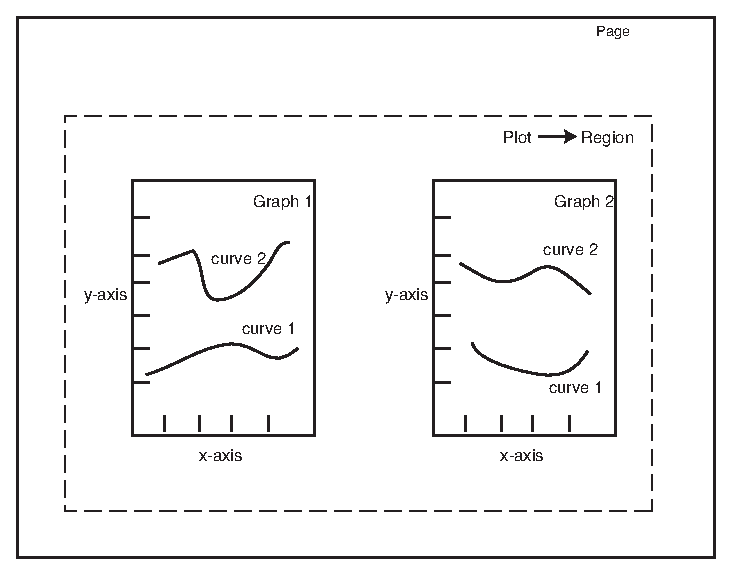
\includegraphics{plot.eps}
  \caption[A plot has a collection of graphs.]
{A plot has a collection of graphs and a graph has a 
collection of curves. A plot becomes visible when it is associated
with some region on the page using the \vn{place} command. Note that
on the actual page the plot/region border is not visible.}
  \label{f:plot}
\end{figure}

Some definitions:
  \vspace*{-3ex}
\begin{description}
\index{Curve|textbf}
\item[Curve] \Newline
A \vn{curve} is a set of (x,y) points to be plotted.
\index{Graph|textbf}
\item[Graph] \Newline
A \vn{graph} consists of horizontal and vertical axes along with a set
of \vn{curve}s that are plotted within the graph. 
\index{Plot|textbf}
\item[Plot] \Newline
A \vn{plot} is essentially a collection of \vn{graphs}.
\index{Page|textbf}
\item[Page] \Newline
The \vn{page} refers to the Xwindow where graphics are displayed or the 
corresponding printed graphics page.
\index{Region}
\item[Region] \Newline
The \vn{page} is divided up into a number of rectangles called
\vn{regions}. \vn{Regions} may overlap.
\end{description}

\index{Template plot}\index{Region}\index{Place command}
\index{Graph}\index{Plot!initialization file}\index{Curve}
The plot initialization file (cf.~Chapter~\ref{c:init}) defines a set
of \vn{template plots}. A \vn{template} defines what type of data is
to be plotted (orbit, beta function, etc.), how many \vn{graphs} there are,
what the scales are for the \vn{graph} axes, how the \vn{graph}s are
laid out, etc.  The plot initialization file also defines a set of
\vn{region}s within the \vn{page}. Any \vn{template plot} can be
placed in any region. Using the \vn{place} command (see
Chapter~\ref{c:command} for a full descriptions of all commands) one
can assign a particular \vn{template plot} to a particular region for
plotting.  The relationship between \vn{region}, \vn{plot},
\vn{graph}, and \vn{curve} is shown graphically in
Figure~\ref{f:plot}.

Figures~\ref{f:plot.page1} and \ref{f:plot.page2} show examples of a
plot \vn{page}. Figure~\ref{f:plot.page1} was generated by defining
two regions called \vn{top} and \vn{bottom} in the plot initialization
file. The \vn{top} region was defined to cover the upper half of the
\vn{page} and the \vn{bottom} region was defined to cover the bottom
half. \vn{Template plots} were defined to plot phase and orbit data
from a defined set of detector elements in the lattice. Each
\vn{template plot} defined two graphs which in both cases where
assigned the names \vn{x} and \vn{y}. The orbit \vn{template plot} was
placed in the \vn{top} region and the phase \vn{template plot} was
placed in the \vn{bottom} region. The horizontal axis numbering is by
detector \vn{index}.  Displayed plots are referred to by the
\vn{region} name (\vn{top} and \vn{bottom} in this case). Individual
graphs and curves are referred to using the nomenclature
\vn{region.graph.curve}. Thus, in this example, the horizontal orbit graph
would be referred to as \vn{top.x}.  Using the \vn{plot} command one
can then specify \vn{who} is plotted. \vn{who} refers to
\vn{measured}, \vn{reference}, \vn{model}, \vn{base}, and/or
\vn{design} data.  Notice that the same \vn{template plot} can be
assigned to different \vn{regions} and the plots in different
\vn{regions} can have different scales for their axes or different
\vn{who}. In the example in Figure~\ref{f:plot.page1}, \vn{who} for
the \vn{top} plot is \vn{model} and for the \vn{bottom} plot it is
\vn{model - design}.

Plots may be referred to by their template name or by the name of the
region they are placed in. For example, the orbit plot in
Figure~\ref{f:plot.page1} may be referred to using the region name
(\vn{top}) or the template name (\vn{orbit}). A template may be placed
in multiple regions.  For example, you may wish to plot the \vn{model}
data for the orbit in one region and the \vn{design} data for the
orbit in another region. In this case the command \vn{scale orbit}
would scale the plots in both regions while to scale the plot in only
one of the regions you would need to use the region name. A graph of a
plot is specified using the format \vn{plot_name.graph_name} where
\vn{plot_name} is a template or region name and \vn{graph_name} is the
name of the graph. For example, if the horizontal orbit graph of the
]\vn{orbit} plot is named \vn{x} then it would be referred to as
\vn{orbit.x} or \vn{top.x}. A curve within a graph is specified using
the format \vn{plot_name.graph_name.curve_name}.

The \vn{use}, \vn{veto}, \vn{restore}, and \vn{clip} commands are used
to control what data is used in fitting the model to the data in the
optimization process (see Chapter~\ref{c:opti}). The general rule is
that these commands only effect measured and reference data. If
plotting \vn{model}, \vn{design} and/or \vn{base} data then the data
will be displayed irregardless. If plotting \vn{meas} and/or \vn{ref} data
then the data displayed will vary with these commands.  \vn{meas} or
\vn{ref} data vetoed for display is also vetoed for fitting.  However,
measured data that is off the vetical or horizontal scale may still be
used by the optimizer unless vetoed with the \vn{veto} or \vn{clip}
command.  If there are data points off the vertical scale then
``**Limited**'' will appear in the upper right-hand corner of the
graph. If plotting measured data then these points off scale will
still be used by the optimizer.

The \vn{x-axis} and \vn{x-scale} commands are used to set the axis
type and scale for each graph. The axis type can be either \vn{index},
\vn{ele_index} or \vn{s} which corresponds to the data index number,
element index number and longitudinal poisition in the lattice (from
element 0) respectively.

Figure~\ref{f:plot.page2} shows another example of a plot \vn{page}.
In this case the \vn{page} was generated by again defining two
vertically stacked regions but in this case the regions have different
heights.  A \vn{template plot} with a single graph was placed in the
bottommost \vn{region}.  This \vn{graph} contains a \vn{key_table}.
A \vn{key_table} is used in conjunction with \vn{single mode} and is
explained in Chapter~\ref{c:single}. A \vn{template plot} containing
five \vn{graphs} was placed in the uppermost region. The uppermost
\vn{graph} of this \vn{template plot} contains a \vn{lat_layout} which
shows the placement of lattice elements.  What elements are displayed
in a \vn{lat_layout} and what shapes they are represented by is
specified in the initialization file. The horizontal scale is
longitudinal position (\vn{s}).  The remaining four graphs show
dispersion and beta data from two different universes representing the
low energy and high energy transport in an energy recovery linac. The
individual data points here (hard to see in this example) have been
slaved to the \vn{lat_layout} and represent the beta and dispersion at
the edges of the displayed elements in the \vn{lat_layout}.


\begin{figure}
  \centering
  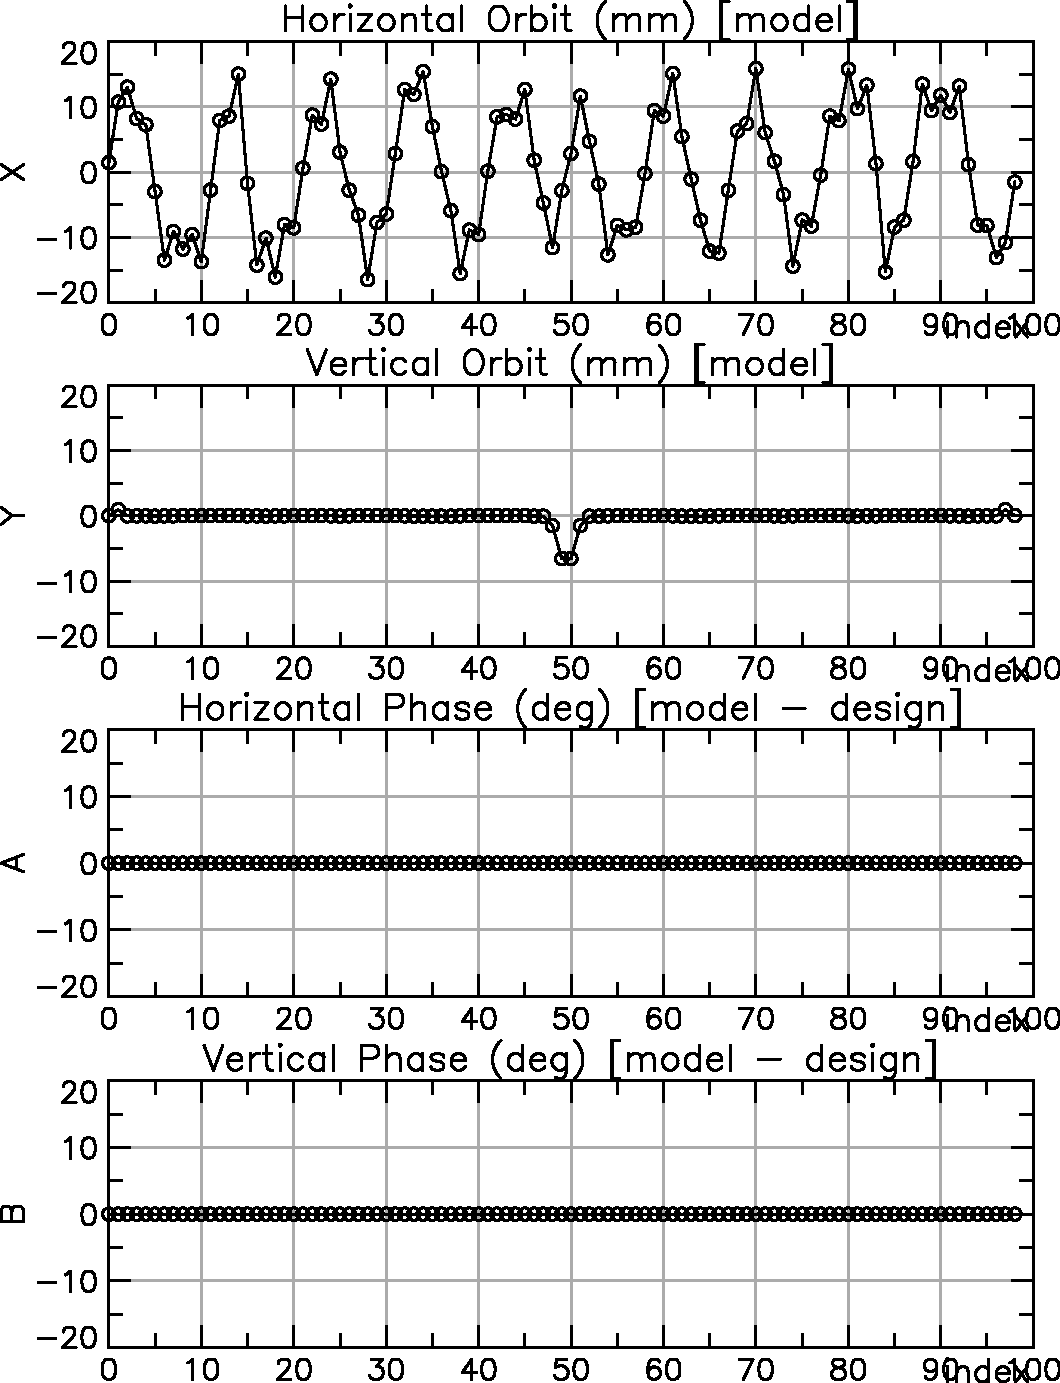
\includegraphics[width=5in]{plot-page1.eps}
  \caption{Example of a plot page}
  \label{f:plot.page1}
\end{figure}

\begin{figure}
  \centering
  \includegraphics[width=5in]{plot-page2.eps}
  \caption{Another example of a plot page.}
  \label{f:plot.page2}
\end{figure}

\vfill
\break
%------------------------------------------------------------------------
\section{Single Character Input}
\index{Single Mode}

Sometimes it is convenient to be able to vary variables using single
key strokes without having to type a carriage return.  With \tao, this
is possible using what is called \vn{single mode}. This is distinct
from \vn{line mode} where commands to \tao are typed at the command
line with a carriage return signaling the end of the command. 

The \vn{single mode} initialization file associates variables with
certain keyboard keys so that when these keys are pressed the value of
the variable is varied. This association between variables and keys is
called a \vn{key table}. See Chapter~\sref{c:single} for more details.

%------------------------------------------------------------------------
\section{Tracking Types}
\index{Tracking!Types}

\index{track_type}
\index{tao_global_struct}
\index{Global%track_type}
The are two types of tracking implemented in \tao: single particle
tracking and many particle multi-bunch tracking.
Single particle tracking is just that, the
tracking of a single particle through the lattice. Many particle
multi-bunch tracking creates a gaussian distribution of particles at
the beginning of the lattice and tracks each particle through the
lattice, including any wakefields. 
Single particle tracking is used by default. The
\vn{global%track_type} parameter (\sref{s:globals}), which is set in
the initialization file, is used to set the tracking.

Particle spin tracking has also been set up for single particle and many
particle tracking. See Sections~\sref{s:globals} and \sref{s:beam.init} for
details on setting up spin tracking.

%------------------------------------------------------------------------
\section{Lattice Calculation}\index{Lattice!calculation of}
\label{s:lat.calc}

After each \tao command is processed, the lattice and ``merit''
function are recalculated and the plot window is regenerated. The
merit function determines how well the \vn{model} fits the measured
data. See Chapter~\ref{c:opti} for more information on the merit
function and its use by the optimizer.

Below are the steps taken after each \tao command execution:
\begin{enumerate}
  \item 
The data and variables used by the optimizer is re-determined. This is
affected by commands such as \vn{use, veto,} and \vn{restore} and any
changes in the status of elements in the ring (e.g. if any elements
have been turned off).
  \item 
If changes have been made to the lattice (e.g. variables changed) then
the model lattice for all universes will be recalculated. The
\vn{model} orbit, linear transfer matrices and twiss parameters are
recalculated for every element. All data types will also be calculated
at each element specified in the initialiation file.  For single
particle tracking the linear transfer matrices and twiss parameters
are found about the tracked orbit. Tracking is
performed using the tracking method defined for each element
(i.e. Bmad Standard, Symplectic Lie, etc...). See the \bmad Reference
manual for details on tracking and finding the linear transfer
matrices and twiss parameters.
  \item 
The \vn{model} data is recalculated from the \vn{model} orbit, linear
transfer matrices, twiss parameters, particle beam information and
global lattice parameters.  Any custom data type calculations are
performed \textit{before} the standard \tao data types are calculated.
  \item 
Any user specified data post-processing is performed in
\vn{tao_hook_post_process_data}.
  \item 
The contributions to the merit function from the variables and data are
computed.
  \item 
Data and variable values are transfered to the plotting structures.
  \item 
The plotting window is regenerated.
\end{enumerate}




\chapter{``Vanilla'' \tao}
\label{c:vanilla_tao}

%----------------------------------------------------------------
\section{Before we start...}
\label{s:before_beginning}

\tao is readily customizable. All the bookkeeping has already been done and all
you need to do custom analysis is write the subroutines pertinent to your
project. However beginners are advised to start with
``out of the box'' \tao while getting to know the program. This tutorial starts
here and will then show you
how to customize \tao for your specific purposes.

\subsection{Getting and Compiling \tao}
\label{s:get_and_compile}

\tao is available in the \cesr CVS area. To checkout a copy type `\cmd{cvs co
tao'} in the directory from where you want to run \tao, hereto refered to as
\vn{ROOT}. If you don't have \cesr
CVS write permission then type `\cmd{cesrcvs co tao}'. This will check out a copy
but will not allow you to check in changes to the code. If you aren't at Wilson
Laboratory then contact David Sagan \cmd{<dcs16@cornell.edu>} to obtain a copy. 

From the newly created \cs{ROOT/tao} directory type `\cmd{gmake}' to create the
libraries and then type `\cmd{gmake -f M.tao}' to create
the ``vanilla'' \tao program. Vanilla \tao is the basic \tao program without any
user customizations. If you are using a custom version of \tao then
follow the compiling directions from the custom \tao author. Keep in mind that
command syntax and usage may vary between custom versions of \tao (this is a
\textit{feature} \textbf{not} a bug!).

Once \tao has compiled go to the subdirectory \cs{ROOT/program} and type
\cmd{../../bin/tao} to run ``vanilla'' \tao. This directory contains all the
configuration files to get everything working. The first time you run the
program it will need to create a digested \bmad lattice file for the included
lattice. This may take a few minutes.

\subsection{Customising \tao}

After you are familiar with the basics of \tao you are ready to fully exploit
the versatility of this wonderful program. See Chapter~\ref{c:custom_tao} to learn
how to do this.

%----------------------------------------------------------------
%----------------------------------------------------------------
\section{In the Beginning...}
\label{s:beginning}

%----------------------------------------------------------------
\subsection{There was the user}

this tutorial assumes you are already familiar with basic particle beam
dynamics and its formalism. There are several books that introduce the topics
very well. The best the author has found so far is \textit{The Physics of
Particle Accelerators} by Klaus Wille. 

\tao is based on the \bmad subroutine library and you should have
a working knowledge of the conventions used by \bmad. \tao can be used ``out of
the box'' so an understanding of the nitty-gritty details of \bmad is not
necessary, however, one should be familiar with the material in Part I
of the \bmad manual.

So, what's \tao good for? Well, virtually everything. It's versatility is that
it's easily exapandable. Think of it as an accelerator design and analysis
environment. The entire \bmad library is at your disposal. But even without any 
customizations \tao will do much analysis. These problems fall into three main
catagories:

\begin{itemize}
\item 
You want to design a lattice subject to various constraints.
\item 
You have some measured data and you want to make a correction. For
example, you want to know what steering strength changes will make an orbit
flat.
\item
You want to simulate what happens to the orbit, beta function,
etc., when you change something in the machine.
\end{itemize}

Programs that are written to solve these types of problems have common
elements: You have variables you want to vary in your model of your
machine, you have "data" that you want to view, and, in the first two
categories above, you want to match the machine model to the data (in
designing a lattice the constraints correspond to the data).

This tutorial is designed to informaly get the user up and running with \tao without
needing to dredge through the entire reference manual. Full command syntax
or greater detail on any topic can be found in the Reference Manual.

%----------------------------------------------------------------
\subsection{Then there was the Super-universe}

Everything known to \tao is placed in an area called the
\textit{super-universe}. Within the \textit{super-universe} lies one or more
universes each containing a particular machine lattice. This allows for the user
to do analysis on multiple machines or multiple configurations of a single
machine at the same time. A \textit{super-universe} consists of the following
parts:

\begin{enumerate}

\item \textbf{A typical universe} \Newline
A universe contains a \bmad lattice plus whatever data one wishes to study
within this lattice (i.e. twiss parameters, orbit, phase \&etc...) . Actually,
there are three lattices within each universe: the \textbf{design
lattice}, \textbf{model lattice} and \textbf{base lattice}. \emph{All lattice changes
specified during a \tao session are incurred on the model lattice.} The design lattice is
fixed at initilization time and serves as a reference point for any elemental
changes incurred during the \tao session. The base lattice also serves as a
reference point but the user can transfer the model lattice over to the base
lattice at any time to create a reference lattice.

Each data point (for example, the horizontal orbit at some detector) has 5 datum
 quantities associated with it: the \textbf{measured data}, \textbf{reference
data}, \textbf{model data}, \textbf{design data} and \textbf{base data}. The
model, design and base data correspond to the appropriate quantity
calculated in its respective lattice above. The measured data corresponds to 
data obtained during a measurement. If doing design work then the desired or
goal
value would be placed here. This data area is also refered to as the constraint during
optimization. The reference data is for observing changes in the data with
respect to a reference.

\item \textbf{Variables} \Newline
Variables control attributes of elements in the model lattice of one or more
universes. They are not the same thing as atributes in lattice elements.
However, they \textit{control} attributes in lattice elements. They are
more akin to \bmad \textit{overlays}. A given variable may control a single 
attribute of one element
in one or more universes. If you want a variable to control a collection of
elements like a \bmad \textit{group} then you need to insert the appropriate
group in your lattice. Variables are what you vary in order to change
your model lattice. You can also change your model lattice by directly changing
and lattice element attribute. However, if you plan on doing any optimization then 
you will need to use variables.

\item \textbf{Key Bindings} \Newline
Key bindings are used in \textit{single mode} where each key
stroke is interpreted without the user having to press the carriage control key.
Each group of keys is bound to a different variable and pressing these keys will
allow you to rapidly change your lattice optics.

\item \textbf{Other stuff in the Super-universe} \Newline
The super-universe also contains information pertaining to global environment variables and
plotting. No need to go into the details here. Part III will
tell you all about this other stuff.
\end{enumerate}

%----------------------------------------------------------------
%----------------------------------------------------------------
\section{Initializing \tao}
\label{s:initializing}

Initialization occurs at startup. There are \emph{four} files used to initialize \tao.
  \vspace*{-3ex}
\begin{enumerate}
  \item \textbf{\textit{your lattice file}} \Newline
    This is your lattice file. ``Vanilla'' \tao comes with its own for
demonstration purposes.
  \item \textbf{tao.init} \Newline 
    This is where global environment variables, data/variable
arrays and key bindings are specified.
  \item \textbf{tao\_plot.init} \Newline
    This is where plotting is set up.
  \item \textbf{tao.startup (optional)} \Newline
    This is a command file that is read in after initialization. Any commands you
want entered in \tao everytime you start up are put here. This is also a great
place to define aliases.
\end{enumerate}

There is no need to go into the details of the initialization files here. If
using Vanilla \tao these are already set up for you in \cs{ROOT/tao/program} and will
setup \tao for use with the included \cesr lattice. If
using a custom version of \tao then the customized \tao author will have already set something
up for you to use. If he or she didn't then go complain to him or her for making
your life difficult and demand proper treatment. If he or she still refuses to
do this for you then it looks like you'll need to read Chapter~\ref{c:custom_tao}
of this tutorial!

\textbf{NOTE: the following chapters will work with vanilla \tao. The commands
entered and plotting output may be different for custom versions.}


%----------------------------------------------------------------
%----------------------------------------------------------------
\section{Getting information from \tao}
\label{s:get_info}

%----------------------------------------------------------------
\subsection{The Plotting Window}

When \tao first starts up you will see a plot window and a command prompt. 
Figure~\ref{f:plot_begin} shows what you will see in the plot window. In the top
two plots you see the \vn{x} and \vn{y} model lattice orbit data. The horizontal
axis is the \cesr BPM index. The horizontal pretzel and L03 vertical bump in
CESR can be clearly 
seen. The slight vertical displacement due to the solenoid can also be seen around 
the IP. The orbit data is for a closed orbit electron (this being a storage
ring). The bottom two plots show the relative 
particle phase. That is, the difference
between the model and design phases (as documented in the plot title as [model -
design]). 

As a first step let's view the absolute model phase. At the \cmd{TAO>} prompt type
\begin{example}
  plot bottom model
\end{example}
This will change the data plotted in the bottom two graphs to just the model.
The plots are now way off scale. Let \tao automatically set the scale by typing
\begin{example}
  scale bottom
\end{example}
As expected, the phase increases approximately linearly as the particle travels
through the ring. Zero phase is halfway through the ring (at L03 in \cesr lingo).
This is always true. Absolute phase is arbitrary so \tao sets the average
phase to zero when generating the data. OK, lets' set this back to relative
phase by typing
\begin{example}
  plot bottom model - design
\end{example}


Let's now look at the beta function by typing
\begin{example}
  place bottom beta
\end{example}
Again, we need to rescale the plots by typing
\begin{example}
  scale bottom
\end{example}
We see the periodic FODO beta function where large horizontal beta corresponds to
small vertical beta and vice versa.

Likewise, we can look at the dispersion in the top two graphs by typing
\begin{example}
  place top eta
  scale top
\end{example}
The plot window should now look like Figure~\ref{f:plot_eta_beta}.

Now let's look at the coupling (C-matrix) by typing
\begin{example}
  place bottom coupling
  scale bottom
\end{example}
We see that there is strong coupling within the CLEO solenoid and virtually no
coupling anywhere else. To zoom in the scale so that we can see the residual
coupling outside the interaction region type
\begin{example}
  clip bottom -0.01 0.01
\end{example}
This will clip or veto all coupling data points outside the range [-0.01,0.01].
Now if we zoom in we can see the fine detail.
\begin{example}
  scale bottom
\end{example}
A better way to ignore the IR region is to use the veto command. First tell \tao
to restore all the coupling data then veto the IR region.
\begin{example}
  restore data coupling all
  veto data coupling 0:5 95:98
  scale
\end{example}
The \vn{0:5 95:98} refers to data indices. Ah ha! There were a few couping data points
outside the IR  that were previously
clipped (notably at the halfway point or L03). We probably would have missed
this if we just used clip. Your plot window should now look like
Figure~\ref{f:plot_coupling_no_IR}.

The x-axis is currently the BPM index number. It is sometimes convenient to plot
the data versus longitudinal position. This is done by typing
\begin{example}
  x-axis all s
\end{example}

Variables can also be plotted provided the proper plot template has been set up
in the plot initialization file (See Section~\ref{s:init_plot} for details on
initializing plotting). Type the following to view the quadrupole k1 values:
\begin{example}
  place bottom quad_k1
\end{example}

The \cmd{all} will apply the change to all plot areas (both top and bottom). In
any of the above commands \cmd{top} or \cmd{bottom} could have been replaced
with \cmd{all}.

\begin{figure}
  \centering
  \includegraphics[width=5in]{plot_page1.psfig}
  \caption{The plot window at startup}
  \label{f:plot_begin}
\end{figure}

\begin{figure}
  \centering
  \includegraphics[width=5in]{plot_eta_beta.psfig}
  \caption{Plotting dispersion and beta function}
  \label{f:plot_eta_beta}
\end{figure}

\begin{figure}
  \centering
  \includegraphics[width=5in]{plot_coupling_no_IR.psfig}
  \caption{Zooming in on the residual coupling outside the IR.}
  \label{f:plot_coupling_no_IR}
\end{figure}

%----------------------------------------------------------------
\subsection{The \cmd{Show} Command}

Anything in the super-universe can be displayed using the \cmd{show} command. To
get a list of the data elements currently defined in \tao type
\begin{example}
  show data
\end{example}
the output should look like:
\begin{example}
   1  orbit
   2  phase
   3  eta
   4  beta
   5  cbar
   6  coupling
\end{example}
There are 6 data types defined in the initialization file. The fifth and sixth are 
closely related. See Part II for an explanation.

To see the data values for the horizontal beta function for \cesr BPMs 1 through
50 type
\begin{example}
  show data beta:x 1:50
\end{example}
Since we haven't changed any elements in the lattice yet the model values equal
the design values. Also note that \vn{beta:x} is actually the a-mode betatron
function. In regions with little or no coupling, the a-mode is almost completely
in the horizontal plane.
 
This is a significant point. The convention in \bmad is to label the twiss
parameters as \vn{x} and \vn{y} but they are actually the \vn{a} and \vn{b}
normal modes. So
in regions of strong coupling \vn{beta:x} does not correspond to \vn{orbit:x}
which is always in the true horizontal lab frame. 
However, if you wish, you can re-label your twiss data planes as \vn{a} and
\vn{b}. Part II shows how to do this. Keep in mind that the twiss
parameters are defined \textit{only for uncoupled betatron motion} so don't even ask for the lab
frame twiss parameters. See the \bmad manual for how to convert
from normal mode coordinates to lab coordinates.

You can also view variables by typing
\begin{example}
  show var
\end{example}
To view the quadrupole k1 values for \cesr quadrupoles 5  and 20 through 30 type
\begin{example}
  sho var quad\_k1 5 20:30
\end{example}
Again, since we haven't changed any quadrupoles the model values are all at their
design values.

You can also see the details of a particular lattice element. To view the details
for quadrupole Q05W type
\begin{example}
  sho ele Q03W
\end{example}

\vn{show var} and \vn{show ele} show two completely different types of
structures in \tao. Elements are the actual lattice elements as known to \bmad. 
Variables are native \tao structures that act kind of like \bmad
\textit{overlays} and only indirectly control the lattice elements.

A list of lattice elements between two elements can be shown by typing (for
example between elements BEGINNING and Q05W)
\begin{example}
  sho lattice beginning Q05W
\end{example}

Command line help is obtained by typing
\begin{example}
  help <command\_name>
\end{example}
where \vn{<command_name>} is the command you want help with.

%----------------------------------------------------------------
%----------------------------------------------------------------
\section{Modifying the Lattice}
\label{s:modify_lattice}

\subsection{Changing a Variable}
\label{ss:change_variable}

Let's change a variable and see what happens to the lattice. We are going to
change a quadrupole strength so we should plot the change in beta and phase.
Type
\begin{example}
  x-axis all index
  place top beta
  place bottom phase
  plot all model - design
  scale
\end{example}

The k1 value can be increased by 0.01 units for quadrupole Q05W by typing
\begin{example}
  change var quad\_k1 5 0.01
  scale
\end{example}
Note the information returned on the command line after the command and the relative changes in
beta and phase in the plot window. This is a vertically focusing quadrupole so
the vertical beta and phase is affected more than the horizontal. The \cmd{0.01}
at the end of the command tells \tao to change this variable by 0.01 units. If
you want to set a variable to a particular value then use a ``@'' before the
value. So, to change this quadrupole k1 to -0.348 type
\begin{example}
  change var quad\_k1 5 @-0.348
\end{example}

\subsection{Putting things back where you found them}
\label{ss:put_it_back}

Let's put this quadrupole back where we found it. We can also modify the quadrupole
by modifying the lattice element directly by typing
\begin{example}
  change ele Q05W k1 d0.0
\end{example}
By modifying the element directly with the \cmd{change ele} command you can
modify any attribute of the element listed in the output of \cmd{show ele Q05W}.
The ``d'' before the value say to set the variable relative to the design value.

If you've changed the lattice around a lot using variables, a great way to set
all variables back to their design values is to type
\begin{example}
  set var all model = design
\end{example}
This only works if you just changed variables. If you changed any elements
directly with the \cmd{change ele} command then this will not work. To set
every attribute of every element back to the design type
\begin{example}
  set lattice model = design
\end{example}
Note that this will also recalculate the data and variable values associated with the
the model lattice to reflect the change so all the bookkeeping is done for you.


%----------------------------------------------------------------
%----------------------------------------------------------------
\section{Running the Optimizer}
\label{s:optimizer}

There are two non-linear optimizers included with \tao: Levenburg - Marquardt,
or `\vn{lm}', and
Differential Evolution, or `\vn{de}'. This example will use the 
Levenburg - Marquardt optimizer which first uses steepest decent to zero in on
the region containing the minimun then uses the inverse-Hessian to converge on
the minimum. See Numerical Recipes in Fortran (or C) book for a detailed
explaination. There's no need to know the details in order to use either
optimizer. Once you set up the problem \tao has the proper wrapper routines to
do the optimization.

Basically, the `\vn{lm}' is typically faster since it uses a dmerit matrix to find
the data deritatives versus each variable before starting the optimization process.
However it assumes the second derivative is fairly smooth, so for very complex function 
spaces the `\vn{de}' may work better. But becuase `\vn{lm}' typically converges much faster
(for function it can handle) it is recommended to try this one first and only use `\vn{de}'
if this one fails. 

\subsection{Fix a Messed Up lattice}
\label{ss:fix_it}

Let's mess the lattice up a little and see if the optimizer can ``fix'' the
lattice. First transfer the ``correct'' lattice to the \vn{meas} data area.
\begin{example}
  set data all meas = design
\end{example}
Now mess up the lattice a bit. We'll be messing with quadrupoles again so plot
beta and phase.
\begin{example}
  place top beta
  place bottom phase
  plot all meas - model
  change var quad\_k1 10 0.001
  change var quad\_k1 21 -0.001
  change var quad\_k1 67 -0.005
  scale
\end{example}
The lattice is now sufficiently screwed up.

Now specify what variables and data to use in the optimization. First type
\begin{example}
  show top10
\end{example}
to see what data is effecting the merit function the most. The merit function is
defined by
\Begineq
  {\cal M} \equiv \sum_{i} w_i \,
    \bigl[ \data_\model(i) -  \data_\meas(i) \bigr]^2 + 
  \sum_{j} w_j \,
    \bigl[ \var_\model(j) - \var_\meas(j) \bigr]^2
  \label{eq:merit}
\Endeq
where $w_{i}$ and $w_{j}$ are the weights given to each component.
The optimizer tries to minimize the merit function by changing the model to look
like the data. From the \vn{top10} output we see that the beta function is effecting 
the merit function the most. Since we
are looking at beta and phase let's only use that data in the optimization.
\begin{example}
  veto data all
  use  data beta all
  use  data phase all
\end{example}
We also know that we need to change quadrupoles to ``correct'' the lattice.
\begin{example}
  veto var all
  use var quad\_k1 all
\end{example}
Note that we need to specify what variables we will be using beforehand in the
initialization files. Raw lattice elements cannot be used by the optimizer. 

Now let's see if we have the optimizer set up correctly.
\begin{example}
  sho optimizer
\end{example}
Whoops! we want to use the Levenburg - Marquardt optimizer so
\begin{example}
  set global optimizer = lm
  sho opt
\end{example}

Now we're ready to run the optimizer or ``fit'' the model to the `measured' data.
\begin{example}
  run
\end{example}
You see the optimizer going through its cycles and it did it! The model is now
``fitted.'' We can see what changes where done to the quadrupoles by typing
\begin{example}
  sho var quad\_k1
\end{example}
The optimizer came very close to finding the ``design'' lattice. However, it changed 
more quadrupoles
than just 10, 21 and 67. This isn't suprising. The optimizer finds the minimun
of the merit function and there are potentially many minimums, or degeneracies.
 It does it's best
not to get stuck in a local minimum and as we can see by the plotted data, the
minimum found is very close -- virtually identical -- to the design lattice optics. 
A good hint as to what variables will be adjusted is the output of \cmd{show optimizer}. 
The top 3
derivatives were not the quadrupoles we adjusted. Nevertheless, the final result
was a darn near perfect match!

\subsection{Now Not Using all of the Variables}
\label{ss:fix_it_not_all}

Alternatively, we could have used only a subsection of the quadrupoles. Say we
know approximately which quadrupoles should be adjusted. So specify these
variables ranges.
\begin{example}
  change var quad\_k1 10 0.001
  change var quad\_k1 21 -0.001
  change var quad\_k1 67 -0.005
  scale
  use var quad\_k1 8:12 20:25 65:70
  run
  sho var quad\_k1 8:12 20:25 65:70
\end{example}
Different quadrupoles than the ones we initially changed were still adjusted
by the optimizer. But the end result is still very close to the design lattice.

\subsection{Lattice Design}
\label{ss:lattice_design}

You may wish to constrain beam
parameters instead of ``fitting'' to data. For example, you could not want
the beta function not to exceed a value in a certain part of the machine. \tao will
also perform this type of optimization.

\fbox{this subsection is yet to be completed!} 

%----------------------------------------------------------------
%----------------------------------------------------------------
\section{Single Mode}
\label{s:single_mode}

Single mode utilizes a simple single character interface between the neural 
network present in your brain and the \tao model lattice. By simply typing
single predefined characters the specified element parameter will be changed by
a certain amount. Neural networks, like your brain, are very efficient at
converging on a nieghborhood around a minimun of a multidimensional non-linear
function space. However, they can be poor at finding the exact minimum. Single mode
utilizes the two optimization schemas (neural network and model fitting) such
that they are applied at the proper times in the evolution of the merit
function.

In other words, you first mess around with the lattice until it get near to the
desired optics layout then you let the optimizer take over to narrow in on the
optimum configuration without requiring it to run all around the
parameter space looking for the nieghborhood around the minimum, which is very
inefficient and time consuming for complex parameter spaces.

\fbox{this section is yet to be completed!} 

%----------------------------------------------------------------
%----------------------------------------------------------------
\section{Where to go from here}
\label{s:where_to_go}

You now have an understanding of the basic abilities of \tao. After this
tutorial, Part II of the \tao Manual should be legible and useful.
The Reference Guide will provide the details of everything mentioned in this tutorial. 
It goes into detail of setting up your own initialization
files and how to use the optimizer. It also includes a complete command
reference with command syntax.

However, you're not yet ready to customize \tao, but this is where the true versatility
of \tao lies. So, onward to the next section and learn how to write your
own custom routines to perform whatever accelerator calculations that strikes your
fancy!

%----------------------------------------------------------------
%----------------------------------------------------------------
%----------------------------------------------------------------
%----------------------------------------------------------------
\chapter{Customizing \tao}
\label{c:custom_tao}

%----------------------------------------------------------------
\section{It's all a matter of Hooks}

The golden rule when extending \tao is that you are only allowed to replace
routines or redefine structures that have the name ``hook'' in them. 
If you have the source code then it's within your power to modify any routine as much 
as you like. However, as time
goes by, and revisions are made to the \tao routines to extend the
usefulness of \tao and to eliminate bugs, only modifying the ``hook'' routines
will ensure that custom changes will
have a minimum impact on the specialized routines that will be written
by various people. 

%----------------------------------------------------------------
\section{Compiling your custom \tao}

As explained in Section~\ref{s:get_and_compile}, the \tao libraries can be
compiled without compiling an executable. Here is where this comes in handy. Since
the standard \tao subroutines have already been made into libraries, all you
need to do is compile and link your custom routines.

There are 9 ``hook'' files located in the \cmd{ROOT/tao/hook} directory. These are
the files you can customize. There are two options here. 
\begin{enumerate}
  \item Change the files directly in \cmd{ROOT/tao/hook}, adding any extra file you
may need, then recompile from the \cmd{ROOT/tao} directory with \cmd{gmake -f M.tao}.
\label{cust_optiin_one}
  \item Copy the hook files to a seprate directory say \cmd{ROOT/my_tao},
adding any extra files you may need, then write a Makefile to compile and link these
routines to the main \tao library.
\label{cust_option_two}
\end{enumerate}
Option~\ref{cust_option_two} is HIGHLY recommended because it keeps the \tao
distribution tree undisturbed and reserves the possibility to create multiple
custom \tao programs using the same vanilla \tao library. This option is used in
the following example.

%----------------------------------------------------------------
\section{An Example}

As an example let's include a new data type called \vn{beam_emittance}. This
will be the non-normalized x and y emittance.. This
data type will behave just like any other data type (i.e. \vn{orbit}, \vn{phase}
etc...). First, we should copy all the hook files to a separate directory call
it \cmd{ROOT/my_tao}. Also include the main program file from the
\cmd{ROOT/tao/program} directory.
(replace \vn{ROOT} with whatever top directory you placed
the \vn{tao} directory in)
\begin{example}
  mkdir ROOT/my_tao
  cp ROOT/tao/hook/*.f90 ROOT/my_tao
  cp ROOT/tao/program/tao_cl.f90 ROOT/my_tao/my_tao_cl.f90
\end{example}
Next we need a Makefile. The \cmd{ROOT/tao/M.tao} 
Makefile is a great starting point.
\begin{example}
  cp ROOT/tao/M.tao ROOT/my_tao/Makefile
\end{example}
Now with your favorite text editor change the following lines in your Makefile
\begin{example}
  LIB\_SRC\_DIRS := ./code ./hook
  OBJ\_SRC\_DIRS := ./program
\end{example}
to
\begin{example}
  LIB\_SRC\_DIRS := ../tao/code
  OBJ\_SRC\_DIRS := ./
\end{example}
This tells gmake to use the tao library that has already been create (from 
\cmd{../tao/code} but the actual library is located at \cmd{../lib/libtao.a})
 and then to compile
all of the hook files, including the main program file (\cmd{my_tao_cl.f90}) in
to object files (everything in \cmd{./}, the current directory).
 Routines and declarations in object files always overide similarly named code in
libraries so this allows for your local hook files to overide the dummy hook
files in the \tao library. The only downside to this method is it clutters your
\cmd{my_tao} directory with object files. You can always remove these object files
with \cmd{gmake clean}.

There are two more lines to alte. change
\begin{example}
  MAIN\_FILE :=
\end{example}
to
\begin{example}
  MAIN\_FILE := ./my\_tao_cl.f90
\end{example}
and finally,
\begin{example}
  MAKEFILE := M.tao
\end{example}
to
\begin{example}
  #MAKEFILE := M.tao !using default name for Makefile
\end{example}
Now you're ready to make your customizations.

This example will only require the modification of one file:
\vn{tao_hook_load_data_array.f90}. The formula for emittance is
\Begineq
  \epsilon = \gamma x^{2} + 2 \alpha x x' + \beta x'^{2}
  \label{e:emittance}
\Endeq
Place the following code in \vn{tao_hook_load_data_array.f90} (in the
\cmd{case select} construct, plus the necessary type declarations)
%\begin{example}
\begin{verbatim}
  case ('emittance:x') 

    datum_value =  ( ele%x%gamma * orb(ix1)%vec(1)**2 + &
		     2 * ele%x%alpha * orb(ix1)%vec(1) * orb(ix1)%vec(2) + &
		     ele%x%beta * orb(ix1)%vec(2)**2)
    
  case ('emittance:y')

    datum_value = ( ele%y%gamma * orb(ix1)%vec(3)**2 + &
		     2 * ele%y%alpha * orb(ix1)%vec(3) * orb(ix1)%vec(4) + &
		     ele%y%beta * orb(ix1)%vec(4)**2)
\end{verbatim}
%\end{example}

Now you just need to declare the data types in the \cmd{tao.init} and
\cmd{tao_plot.init} files. For the sake of this example, modify the
initialization files used for this tutorial.
\begin{example}
  cp ROOT/tao/program/*.init ROOT/my_tao
  cp ROOT/tao/program/*.lat ROOT/my_tao
\end{example}

In \cmd{ROOT/my_tao/tao.init} add the following lines to the data declarations
section
\begin{example}
  &tao_d2_data
    d2_data%name = "emittance" 
    universe = 0 
    n_d1_data = 2
  /

  &tao_d1_data
    ix_d1_data = 1
    d1_data%name = "x"  
    default_weight = 1
    ix_min_data = 0 
    ix_max_data = 99  
    data(0)%name = "SAME: orbit:x"
    data(0)%ele_name = "SAME: orbit:x"
  /

  &tao_d1_data
    ix_d1_data = 2
    d1_data%name = "y"  
    default_weight = 1
    ix_min_data = 0 
    ix_max_data = 99  
    data(0)%name = "SAME: orbit:x"
    data(0)%ele_name = "SAME: orbit:x"
  /
\end{example}
and increase \vn{n_d2_data_max} to 7 in the \vn{tao_params} declaration.

In \cmd{ROOT/my_tao/tao_plot.init} add the following lines to the end of the
file
\begin{example}
  &tao_template_plot
    plot%name = 'emittance'
    plot%x%min =   0
    plot%x%max = 100
    plot%x%major_div = 10
    plot%x%label = ' '
    plot%x_axis_type = 'index'
    plot%n_graph = 2
  /
  
  &tao_template_graph
    graph%name = 'x'
    graph_index = 1
    graph%box = 1, 2, 1, 2
    graph%title = 'Horizontal Emittance (microns)'
    graph%margin =  0.15, 0.06, 0.12, 0.12, '%BOX'
    graph%y%label = 'x'
    graph%y%max =  15
    graph%y%min =  0.0
    graph%y%major_div = 4
    graph%n_curve = 1
    curve(1)%data_source = 'data_array'
    curve(1)%data_type   = 'emittance:x'
    curve(1)%units_factor = 1e6 !convert from meters to microns
  /

  &tao_template_graph
    graph%name = 'y'
    graph_index = 2
    graph%box = 1, 1, 1, 2
    graph%title = 'Vertical Emittance (microns)'
    graph%margin =  0.15, 0.06, 0.12, 0.12, '%BOX'
    graph%y%label = 'Y'
    graph%y%max =  15
    graph%y%min =  0.0
    graph%y%major_div = 4
    graph%n_curve = 1
    curve(1)%data_source = 'data_array'
    curve(1)%data_type = 'emittance:y'
    curve(1)%units_factor = 1e6 !convert from meters to microns
  /
\end{example}

We are now ready to compile and then run the program. The \tao library should have
already been created (in section~\ref{s:get_and_compile}) so all you need to do is
\begin{example}
  cd ROOT/my_tao
  gmake
  ../bin/my_tao_cl
\end{example}
Notice that the name of the custom \tao program is \cmd{my_tao_cl}. If you run 
`\cmd{tao}' then you will run ``vanilla'' \tao.

After your custom \tao initializes type
\begin{example}
  place bottom emittance
  scale
\end{example}
Your plot should look like Figure~\ref{f:plot_emittance}.

The emittance (as calculated) is not constant. This is due to dispersion and
coupling
throughout the ring. \bmad provides a routine to find the emittance that
includes dispersion and coupling.

\begin{figure}
  \centering
  \includegraphics[width=5in]{plot_emittance.psfig}
  \caption{Custom data type: non-normalized emittance}
  \label{f:plot_emittance}
\end{figure}

This example just illustrates one of the customizations you can perform on \tao.
Part III, Programmer's Guide lays out all of the hook files and provides pointers
for various customizations.


\part{Reference Guide}\label{ref_guide}

\chapter{Data types}
\label{c:data_types}

%------------------------------------------------------------------------
\section{How Tao Handles Data}
\index{Data}

As explained in Section~\sref{s:data}, \tao has special structures
to hold data to be analyzed. Any lattice or beam parameters that are
needed to be analyzed or plotted must have a data type defined for
it. In general, a data type can be any type of parameter that is not
necessarily measurable in a real world machine. For example, there is
an orbit data type and a BPM data type. The orbit data is the real
x,y,z position of a particle in the lab frame whereas the BPM data is
the x and y reading on a simulated beam position monitor that includes
any offsets, tilts and noise.

\tao includes many different data types already predefined and
these can be classified into three main catagories:
\begin{enumerate}
  \item \textbf{Lattice Parameters} \Newline
    For example lattice twiss parameters, coupling and floor position.
  \item \textbf{Single Particle Properties} \Newline
    For example particle orbit, BPM reading and phase advance.
  \item \textbf{Bunch Properties} \Newline
    For example bunch sigmas, emittance and beam twiss parameters.
\end{enumerate}
For a given data type the method used to calculate the datum can vary
depending on the tracking type. For {\it single} particle tracking all
data is found from the lattice parameters except for the orbit
data. For \textit{particle bunch} or \textit{macroparticle bunch}
tracking some of the datums are found from the particle distribution
using the appropriate \bmad routines. For example, with single
particle tracking the beta function is found from the lattice
transport matrix, however, with particle or macroparticle tracking the
beta function is found from the particle distribution using the
formula
\begin{equation}
  \beta = \frac{<x^{2}>}{\sqrt{<x^{2}> <x'^{2}> - <x x'>^{2}}}.
\end{equation}
The next section will describe how each predefined data type is
calculated.  Custom data types need not fall into one of the above
catagories and can be any real number as calculated in the appropriate
ook routine.

Also associated with a datum are two lattice elements called
\vni{ele} and \vni{ele0}. The \vni{data_types} are divided into two
categories: Those that are \vni{relative} and those that are not.  A
\vni{relative} \vni{data_type} means that the \vni{model} value for that
datum is determined by a difference between elements. For example, for
\vn{phase.a} the \vn{model} value is
\begin{example}
  model_value = \(\phi\sb{x}\)(ele) - \(\phi\sb{x}\)(ele0)
\end{example}
If there is no \vn{ele0} associated with a datum then the model value is
\begin{example}
  model_value = \(\phi\sb{x}\)(ele) - \(\phi\sb{x}\)(0)
\end{example}
where $\phi_x(0)$ is the phase at the 0\Th element (which is always at
0 radians).
\index{Data!Relative}

For datums with \vni{non-relative} \vn{data_types} if there is also an
associated \vni{ele0} element then the \vn{model} value is dependent
upon the \vni{merit_type}. For example, with a \vn{beta.x}
\vn{data_type} the model value is determined by Table~\ref{t:eval2}
where \vn{i} goes from the \vn{ele} index to the \vn{ele0} index.
\begin{table}[ht]
\centering
{\tt
\begin{tabular}{|l|l|l|} \hline
  {\it Merit\_Type}       & {\it Model Value} \\ \hline 
  \vni{min}     & $\min \beta_x(i)$ \\ \hline 
  \vni{max}     & $\min \beta_x(i)$ \\ \hline 
  \vni{abs_min} & $\min |\beta_x(i)|$ \\ \hline 
  \vni{abs_max} & $\min |\beta_x(i)|$ \\ \hline 
  \vni{target}  & {\it Error}   \\ \hline 
\end{tabular}
}
\caption{\vn{Model} evaluation.}
\label{t:eval2}
\end{table}

%------------------------------------------------------------------------
\section{Tao Data Types}\index{Data!Data Types}
\label{s:data_types}

Table~\ref{t:data_types} lists the predefined data types in \tao.

\vn{wire} data simulates the measurement of a wire scanner. The angle specified
is the angle of the wire with respect to the horizontal axis. The measurement
then measures the second momment $<uu>$ along an axis which is 90 degrees off of
the wire axis. For example, \vn{wire:90} is a wire scanner oriented in the
vertical direction and measures the second moment of the beam along the
horizontal axis, $<xx>$. The resultant data is not the beam size, but the beam
size squared.

Data types marked \vn{global} do not have any particular elements
associated with them.

\index{Data!Calculation Method}

\index{unstable_ring}\index{beta}\index{alpha}\index{eta}\index{eta}
\index{etap}\index{phase}\index{orbit}\index{bpm}\index{wire}\index{spin}
\index{cbar}\index{coupling}\index{floor}\index{r}\index{t}\index{tt}
\index{i5a_e6}\index{i5b_e6}\index{s_position}\index{e_tot}
\index{unstable_ring}\index{emittance}\index{chrom}\index{norm_emittance}
\index{sigma}\index{dpx_dx}\index{dpy_dy}\index{dpz_dz}\index{dpa_da}
\index{dpb_db}
\begin{table}[ht] 
\centering 
{\tt\small
\begin{tabular}{|l|l|l|} \hline
  {\it Data\_Type}              & {\it Description}                  &          \\ \hline 
    alpha.x, alpha.y            & Projected Alpha Function           &          \\ \hline 
    alpha.a, alpha.b, alpha.z   & Normal-Mode Alpha Function         &          \\ \hline 
    e\_tot                      & Beam Total Energy                  &          \\ \hline
    beta.x, beta.y              & Projected Beta Function            &          \\ \hline 
    beta.a, beta.b, beta.z      & Normal-Mode Beta Function          &          \\ \hline 
    bpm.x, bpm.y                & Transverse BPM reading             &          \\ \hline 
    eta.x, eta.y                & Projected Dispersion               &          \\ \hline 
    eta.a, eta.b                & Normal-Mode Dispersion             &          \\ \hline 
    etap.x, etap.y              & Projected Dispersion derivative    &          \\ \hline 
    etap.a, etap.b              & Normal-Mode Dispersion derivative  &          \\ \hline 
    momentum\_compaction        & Momentum compaction factor         & relative \\ \hline
    orbit.x, orbit.y            & Transverse orbit                   &          \\ \hline 
    orbit.p\_x, orbit.p\_y      & Tranverse momenta                  &          \\ \hline 
    orbit.z, orbit.z\_p         & Longitudinal orbit and momenta     &          \\ \hline 
    phase.a, phase.b            & Betatron phase                     & relative \\ \hline 
    phase\_frac\_diff           & Fractional phase difference (x-y)  & relative \\ \hline
    \begin{tabular}{@{}l}     
      spin.polarization, \\ 
      spin.theta, spin.phi 
    \end{tabular} 
                          & Particle spin                      &          \\ \hline 
    \begin{tabular}{@{}l}     
      cbar.11, cbar.12, \\ 
      cbar.21, cbar.22 
    \end{tabular} 
                          & Coupling                          &          \\ \hline 
    \begin{tabular}{@{}l}   
      coupling.11b, coupling.12a, \\ 
      coupling.12b, coupling.22a 
    \end{tabular} 
                          & Coupling                          &          \\ \hline 
    floor.x, floor.y, floor.z
                          & Global (``floor'') position       & relative \\ \hline 
    floor.theta           & Global (``floor'') angle          & relative \\ \hline 
    r.$ij$                & 
                           \begin{tabular}{l}
                             Term in linear transfer map \\
                             $1 \le i,j \le 6$
                           \end{tabular}
                                                              & relative \\ \hline 
    t.$ijk$               & 
                           \begin{tabular}{l}
                             Term in 2\Nd order transfer map \\
                              $1 \le i,j,k \le 6$
                           \end{tabular} 
                                                              & relative \\ \hline 
    tt.$ijklm\ldots$      & 
                           \begin{tabular}{l}
                             Term in n\Th order transfer map \\
                              $1 \le i,j,k,\ldots \le 6$
                           \end{tabular} 
                                                              & relative \\ \hline 
    i5a\_e6, i5b\_e6      & Normalized I5 radiation integral  &          \\ \hline
    s\_position           & longitudinal length constraint    & relative \\ \hline 
    unstable\_ring        & Nonzero if a ring is unstable     & global   \\ \hline
    \begin{tabular}{@{}l}
      emittance.x, emittance.a \\
      emittance.y, emittance.b \\
      emittance.z \\
    \end{tabular}
                          & Emittance                        & global   \\ \hline
    \begin{tabular}{@{}l}  
      norm\_emittance.x, norm\_emittance.a \\
      norm\_emittance.y, norm\_emittance.b \\
      norm\_emittance.z \\
    \end{tabular} 
                          & Normalized Beam Emittance         &          \\ \hline 
    \begin{tabular}{@{}l}
      chrom.a, chrom.b  \\
    \end{tabular}
                          & Chromaticity for a ring           & global   \\ \hline
    \begin{tabular}{@{}l}   
      sigma.x, sigma.p\_x \\ 
      sigma.y, sigma.p\_y \\
      sigma.z, sigma.p\_z \\
    \end{tabular} 
                          & Bunch size                        &          \\ \hline 
    \begin{tabular}{@{}l}   
      multi\_turn\_orbit.x, multi\_turn\_orbit.p\_x \\ 
      multi\_turn\_orbit.y, multi\_turn\_orbit.p\_y \\
      multi\_turn\_orbit.z, multi\_turn\_orbit.p\_z \\
    \end{tabular} 
                          & Bunch size                        &          \\ \hline 
    \begin{tabular}{@{}l}  
      dpx\_dx, dpa\_da \\
      dpy\_dy, dpb\_db \\
      dpz\_dz \\
    \end{tabular} 
                          & <x p\_x> / <x\^2> \& Etc...       &          \\ \hline 
    wire.<angle>                & Wire Scanner with wire angle <angle>
                                                               &          \\ \hline
\end{tabular}
} 
\label{t:data_types}
\caption{Predefined Data Types}
\end{table}

\vfill \break
{\vfill}



\chapter{Optimization}
\label{c:opti}

%------------------------------------------------------------------------
\section{Lattice Corrections}

Examples of lattice corrections include flattening the orbit and
adjusting quadrupoles to correct the measured betatron phase. The
general idea is to vary an appropriate set of \vn{variables} with the
aim of minimizing a merit function \vn{M} that is a measure of how
well \vn{data_model}, the data as calculated from the \vn{model} fits
\vn{data_meas}, the measured data
\Begineq
  {\cal M} \equiv \sum_{i} w_i \,
    (\data\_\model(i) -  \data\_\meas(i))^2 + 
  \sum_{j} w_j \,
    (\var\_\model(j) - \var\_\meas(j))^2
  \label{m1}
\Endeq
\vn{var_model} is the value of a variable in the \vn{model} and
\vn{var_meas} is the value as measured at the time the data was taken
and the sum \vn{j} runs over all variables that are allowed to be
varied to minimize \vn{M}. The second term in the merit function
prevents degeneracies (or near degeneracies) in the problem which
would allow \tao to find solutions where \vn{data_model} matches
\vn{data_measured} with the \vn{var_model} having ``unphysical''
values (values far from \vn{var_meas}. The weights $w_i$ and $w_j$
need to be set depending upon how accurate the measred data is
relative to how accurate the calibrations for measuring the
\vn{var_meas} values are. With the second term in the merit function
the number of constraints (number of terms in the merit function) is
always larger than the number of variables and degeneracies can never
occur. 

The algorithm used to vary the \vn{var_model} variables to minimize
\vn{M} is called an \vn{optimizer}. In \vn{command line mode} the
\vn{run} command is used to invoke an \vn{optimizer}. In \vn{single
mode} the \vn{g} key starts an optimizer and the \vn{.} key stops it.
Running an optimizer is also called ``fitting'' since one is tring to
get the \vn{data_model} to be equal to the \vn{data_meas}. With orbits
this is also called ``flattening'' since one generally wants to end up
with an orbit that is on--axis.

In a correction one wants to change the machine variables so that the
measured data corresponds to the design values \vn{data_design}. Thus
the change in the data that one wants is
\begin{example}
  data_change = data_design - data_meas
\end{example}
Once a fit has been made, and presuming that the \vn{data_model} is
resonably close to the \vn{data_meas} this data change within the
\vn{model} lattice can be accomplished by changing the variables by
\begin{example}
  var_change = var_design - var_model
\end{example}
This assumes the system is linear. For many situations this is true
since typically \vn{var_change} is ``small''. Since the variables have
a measrued value of \vn{var_meas} the value that the variables should
be set to is
\begin{example}
  var_final = var_meas + (var_design - var_model)
\end{example}
Notice that the fitting process is independent of the \vn{design}
lattice. It is only when calculating the corrections to the
variables that the \vn{design} lattice plays a roll. 

Sometimes it is desired to fit to changes in data as opposed to the
absolute value of the data. For example, when closing an orbit bump
knob what is important is the difference in orbits before and after
the bump knob is varied. Designating one of these orbit the
\vn{reference}, the appropriate merit function is
\begin{alignat}{1}
  {\cal M} = &\sum_{i} w_i \,
    \left[ \bigl( \data\_\model(i) - \data\_\design(i) \bigr) - 
      \bigl( \data\_\meas(i) - \data\_\reference(i) \bigr) \right]^2 + \CRNO
  &\sum_{j} w_j \,
    \left[ \bigl( \var\_\model(j) - \var\_\design(j) \bigr) -
     \bigl( \var\_\meas(i) - \var\_\reference(i) \bigr) \right]^2 
  \label{m2}
\end{alignat}
where \vn{data_ref} and \vn{var_ref} refer to the reference
measurement.  This merit function is acceptable if the reference data
is taken with the machine reasonably near the design setup so that
nonlinearities can be ignored. If this is not the case then the
fitting becomes a two step process: The first step is to fit the
\vn{model} to the \vn{reference} data using the merit function of
\Eq{m1}. The \vn{base} lattice is then set equal to the \vn{model}
lattice. The second step is to fit the model using the merit function
\begin{alignat}{1}
  {\cal M} = &\sum_{\data: i} w_i 
    \left[ (\data\_\model(i) - \data\_\base(i)) - 
      (\data\_\meas(i) - \data\_\reference(i)) \right]^2 + \CRNO
  &\sum_{\var: j} w_j 
    \left[ (\var\_\model(j) - \var\_\base(j)) -
     (\var\_\meas(i) - \var\_\reference(i)) \right]^2 
  \label{m3}
\end{alignat}

Control of what data and what variables are to be used in the fitting
process is controlled by the \vn{use}, \vn{veto}, \vn{restore}, and
\vn{clip} commands.

%------------------------------------------------------------------------
\section{Lattice Design}

Lattice design is the process of calculating \vn{variable} strengths
to meet a number of criteria called constraints. For example, one
constraint could be that the beta function in some part of the lattice
not exceed a certain value. In this case we can proceed as was done
for lattice correction and define a merit function to be minimized:
\Begineq
  {\cal M} = \sum_{\mbox{constraints} i} w_i \, C_i^2
\Endeq
The general form of the $C_i$ constraint values is
\Begineq
  C = 
    \begin{cases}
    (\mbox{Model} - \mbox{Target})  & Condition \\
    0                               & Otherwise
    \end{cases}
\Endeq
where \vn{model} is the value as calculated from the \vn{model}
lattice and \vn{target} is some given number. Part of the optimization
process is in deciding what the values should be for the \vn{targets}.
The \vn{condition} needed for a non--zero $C_i$ is dependent upon the
\vn{type} of the constraint. There are five constraint types:
\begin{table}[h]
\centering
{\tt
\begin{tabular}{|l|l|l|} \hline
  {\it Constraint Type}  & $C$ & {\it Condition for non-zero $C$} \\ \hline 
  \vn{target}     & \vn{model} - \vn{target}   & \vn{model} $\ne$ \target     \\ \hline 
  \vn{min}        & \vn{model} - \vn{target}   & \vn{model} $<$ \vn{target}   \\ \hline 
  \vn{max}        & \vn{model} - \vn{target}   & \vn{model} $>$ \vn{target}   \\ \hline 
  \vn{abs_min}    & |\vn{model}| - \vn{target} & |\vn{model}| $<$ \vn{target} \\ \hline 
  \vn{abs_max}    & |\vn{model}| - \vn{target} & |\vn{model}| $>$ \vn{target} \\ \hline 
\end{tabular}
}
\caption{Constraint Type List.}
\label{t:con_type}
\end{table}

Since lattice design and lattice corrections are very similar, \tao
combines the two into one generalized correction process. With \tao
the constraint \vn{model} values are identified with the
\vn{data_model} and the \vn{target} values are identified with the \vn{data_meas}.
The different types of \vn{data} that \tao knows about is called the data's \vn{type}

\begin{table}[h] \centering {\tt
\begin{tabular}{|l|l|l|} \hline
  {\it Constraint/Data Type} & {\it Description}     &          \\ \hline 
    beta:x, beta:y    & Twiss parameter              &          \\ \hline 
    alpha:x, alpha:y  & Twiss parameter              &          \\ \hline 
    eta:x, eta:y      & Dispersion                   &          \\ \hline 
    etap:x, etap:y    & Dispersion derivative        &          \\ \hline 
    phase:x, phase:y  & Betatron phase               & relative \\ \hline 
    orbit:x, orbit:y  & Particle orbit               &          \\ \hline 
    cbar:11, cbar:12, cbar:21, cbar:22 
                      & Coupling                     &          \\ \hline 
    floor:x, floor:y, floor:z
                      & Global (``floor'') position  & relative \\ \hline 
    floor:theta       & Global (``floor'') angle     & relative \\ \hline 
    r56            & Term in linear transfer map     & relative \\ \hline 
    t566           & Term in 2nd order transfer map  & relative \\ \hline 
    s              & Longitudinal length constraint  & relative \\ \hline 
\end{tabular}
} \caption{Constraint List.}  \label{t:cons}
\end{table}

\chapter{Tao Initialization}\index{Initialization}
\label{c:init}

\tao is customized for specific machines and specific calculations
using input files and custom software routines. Writing custom
software is covered in the programmer's guide section. This chapter
covers the input files.

In general, the input files tell \tao:
\begin{example}
  1) What the "standard" variables should be.
  2) What the "standard" data is.
  3) What to plot and where to plot it.
\end{example}

\tao first looks for input files in the current directory and then
looks in a directory pointed to by the environmental variable
\vn{TAO_INIT_DIR}.

Initialization parameters are read in from a file using Fortran
namelist input. Fortran namelist breaks up the input file into
blocks. The first line of a namelist block starts with an ampersand
``\&'' followed by the block identifying name. Variables are assigned
using an equal sign ``='' and the end of the block is denoted by a
slash ``/'' For example:
\begin{example}
  &this_block_name
    var1 = 0.123   ! exclamation marks are used for comments
    var2 = 0.456
  /
\end{example}
Variables that have default values can be omitted from the block.  The
order of the variables inside a block is irrelevant.  In between
namelist blocks all text is ignored. Inside a block comments may be
included by using an exclamation mark ``!''.

Note: string variables are case sensitive.

%-----------------------------------------------------------------
\section{Beginning Initialization}
\index{Initialization!beginning}
\label{s:init_global} 


\index{tao_start}
\index{tao.init}
\index{lattice_file}
\index{data_file}
\index{var_file}
\index{plot_file}
\index{single_mode_file}
\index{startup_file}
\index{n_universes}
\index{startup_single_mode}
The initialization starts with an initialization file named
\vn{tao.init}.  \vn{tao.init} needs to have a \vn{tao_start} namelist
block with the following syntax:
\begin{example}
  &tao_start
    lattice_file      = "<file_name>"  ! Default = this file.
    data_file         = "<file_name>"  ! Default = this file.
    var_file          = "<file_name>"  ! Default = this file.
    plot_file         = "<file_name>"  ! Default = this file.
    single_mode_file  = "<file_name>"  ! Default = this file.
    startup_file      = "<file_name>"  ! Default = "tao.startup"
    n_universes       = <integer>            ! Number of universes. Default = 1.
    init_name      = "<init_name>" !Default = 'Tao"
  /
\end{example}
\vn{n_universes} is the number of universes to be created.  \vn{init_name} is
for naming the initialization. This is useful to distinguish between multiple
initialization files with custom versions of \tao.  The other parameters specify
which files to find the other initialization namelists. The following sections
describe each of these initialization namelists and their locations are listed
in table \ref{t:init_files}.

\index{tao_design_lattice}
\index{tao_params}
\index{tao_coupled_uni_init}
\index{tao_beam_init}
\index{tao_macro_init}
\index{tao_var}
\index{tao_d2_data}
\index{tao_d1_data}
\index{tao_plot_page}
\index{tao_template_plot}
\index{tao_template_graph}
\index{element_shapes}
\index{key_bindings}
\begin{table}[h]
\centering {\tt
\begin{tabular}{|l|l|l|l|} \hline
  {\it Namelist} & {\it File Name} & {\it Initialized here}  & {\it Section} \\ \hline
  \vn{tao_design_lattice}   & \vn{lattice_file} & lattice files       & \ref{s:init_lat}    \\ \hline
  \vn{tao_params}           & 'tao.init' & Global Variables    & \ref{s:globals}     \\ \hline
  \vn{tao_coupled_uni_init} & 'tao.init' & Coupled Universes   & \ref{s:coupled_uni} \\ \hline
  \vn{tao_beam_init}        & 'tao.init' & Particle beam       & \ref{s:beam_init}   \\ \hline
  \vn{tao_macro_init}       & 'tao.init' & Macroparticle beam  & \ref{s:macro_init}  \\ \hline
  \vn{tao_var}              & \vn{var_file}     & Variables           & \ref{s:init_var}    \\ \hline
  \vn{tao_d2_data}          & \vn{data_file}    & Data                & \ref{s:init_data}   \\ \hline
  \vn{tao_d1_data}          & \vn{data_file}    & Data                & \ref{s:init_data}   \\ \hline
  \vn{tao_plot_page}        & \vn{plot_file}    & Plotting            & \ref{s:init_plot}   \\ \hline
  \vn{tao_template_plot}    & \vn{plot_file}    & Plotting            & \ref{s:init_plot}   \\ \hline
  \vn{tao_template_graph}   & \vn{plot_file}    & Plotting            & \ref{s:init_plot}   \\ \hline
  \vn{element_shapes}       & \vn{plot_file}    & Plotting            & \ref{s:init_plot}   \\ \hline
  \vn{key_bindings}         & \vn{single_mode_file} & Single Mode     & \ref{s:init_single}   \\ \hline
\end{tabular}}
\caption{Table of \vn{tao} Initialization Namelists}
\label{t:init_files}
\end{table}


%-----------------------------------------------------------------
\section{Lattice Initialization}\index{Initialization!Lattice}
\label{s:init_lat} 

The \vn{lattice_file} variable in the \vn{tao_start} namelist is the
name of the file with the \vn{tao_design_lattice} namelist that
defines where the lattice input files are. The \vn{tao_design_lattice}
namelist has the form
\index{tao_design_lattice}
\index{design_lattice}
\index{design_lattice!file}
\index{design_lattice!parser}
\begin{example}
  &tao_design_lattice
    taylor_order = <num>
    design_lattice(i)%file = "<lattice_file>"
    design_lattice(i)%parser = "<parser>"
  /
\end{example}
\vn{taylor_order} is the order of the Taylor maps. This will override
the Taylor order set in the lattice files. \vn{i} refers to the
universe index, \vn{<lattice_file>} is the name of an input lattice
file and \vn{<parser>} is the name of the parser to use. Possible
choices for \vn{<parser>} are:
\index{bmad}\index{xsif}\index{digested}
\begin{example}
  bmad      ! For a standard bmad lattice file. This is the default.
  xsif      ! For an xsif lattice file.
  digested  ! For a digested BMAD file.
\end{example}

Example:
\begin{example}
  &tao_design_lattice
    design_lattice(1)%file = "this.lat"          ! Default: Use the bmad parser 
    design_lattice(2)      = "that.lat", "xsif"  ! For universe \#2
  /
\end{example}

%-----------------------------------------------------------------
\section{Initializing Globals}\index{Initialization!Globals}
\label{s:globals} 

Global variables are initialized in the \vn{data_and_var_file} using a
namelist block named \vn{tao_params} The syntax of this block is:
\index{tao_params}\index{n_v1_var_max}\index{n_d2_data_max}
\index{n_data_max}\index{n_var_max}\index{global}\index{bmad_com}
\index{csr_com}
\begin{example}
  &tao_params
    n_v1_var_max  = <integer>   ! number of v1 data structures.
    n_d2_data_max = <integer>   ! number of d2 data structures.
    n_data_max    = <integer>   ! Total number of data points
    n_var_max     = <integer>   ! Total number of variables.
    global        = <tao_global_struct>  ! global parameters
    bmad_com      = <bmad_com_struct> ! Bmad global parameters
    csr_com       = <csr_common_struct>  ! CSR global parameters
  /
\end{example}
Example:
\begin{example}
  &tao_params
    n_v1_var_max  = 5
    n_d2_data_max = 6
    n_data_max    = 2000
    n_var_max     = 2000
    global%optimizer = "lm"  ! Set the default optimizer.
  /
\end{example}
\vn{n_d2_data_max} and \vn{n_v1_var_max} are the maximum number of
\vn{d2_data} and \vn{v1_var} structures needed. \vn{n_data_max} is the
maximum number of datums needed and \vn{n_var_max} is the maximum
total number variables used. 

The \vn{tao_global_struct} structure contains \tao global parameters.
\index{y_axis_plot_dmin}\index{u_view}\index{n_opti_cycles}\index{ix_key_bank}
\index{n_key_table_max}\index{n_lat_layout_label_rows}\index{phase_units}
\index{bunch_to_plot}\index{n_curve_pts}\index{random_seed}\index{n_write_file}
\index{track_type}\index{prompt_string}\index{Optimization!setting the optimizer}
\index{default_key_merit_type}\index{write_file}\index{var_limits_on}
\index{plot_on}\index{auto_scale}\index{opt_with_ref}\index{opt_with_base}
\index{single_mode}\index{init_opt_wrapper}\index{lm_opt_deriv_reinit}
\index{label_lattice_elements}\index{label_keys}\index{derivative_recalc}
\index{lattice_recalc}\index{init_plot_needed}
\index{valid_plot_who}\index{print_command}\index{default_init_file}
\index{current_init_file}\index{var_out_file}\index{opt_var_out_file}
\begin{example}
type tao_global_struct
  real(rp) :: y_axis_plot_dmin = 1e-4    ! Minimum y_max-y_min allowed for a graph.
  real(rp) :: lm_opt_deriv_reinit = -1   ! Reinit derivative matrix cutoff
  real(rp) :: de_lm_step_ratio = 1       ! Scaling for step sizes between DE and LM optimizers.
  integer :: u_view = 1                  ! Which universe we are viewing.
  integer :: n_opti_cycles = 20          ! number of optimization cycles
  integer :: ix_key_bank = 0             ! For single mode.
  integer :: n_key_table_max = 0         ! Maximum key table index.
  integer :: n_lat_layout_label_rows = 1 ! How many rows with a lat_layout
  integer :: phase_units = radians\$     ! Phase units on output.
  integer :: bunch_to_plot = 1           ! Which bunch to plot
  integer :: n_curve_pts = 401           ! Number of points for plotting a smooth curve
  integer :: random_seed = 0             ! use system clock by default
  integer :: n_write_file = 0            ! used for indexing 'show write' files
  character(16) :: track_type = 'single' ! or 'beam', 'csr', or 'macro' 
  character(16) :: prompt_string = 'Tao'
  character(16) :: optimizer = 'de'      ! optimizer to use.
  character(16) :: default_key_merit_type
  character(80) :: write_file = 'tao_show.dat'
  logical :: var_limits_on = .true.      ! Respect the variable limits?
  logical :: plot_on = .true.            ! Do plotting?
  logical :: auto_scale = .false.        ! Automatically scale and x-scale the plots?
  logical :: opt_with_ref = .false.      ! use reference data in optimization?
  logical :: opt_with_base = .false.     ! use base data in optimization?
  logical :: single_mode = .false.
  logical :: optimizer_running 
  logical :: init_opt_wrapper = .true.
  logical :: label_lattice_elements = .true. ! For lat_layout plots
  logical :: label_keys = .true.             ! For lat_layout plots
  logical :: derivative_recalc = .true.      ! Recalc before each optimizer run?
  logical :: lattice_recalc = .true.         ! recalculate the lattice?
  logical :: init_plot_needed = .true.       ! reinitialize plotting?
  character(16) :: valid_plot_who(10)        ! model, base, ref etc...
  character(40) :: print_command = 'awprint'
  character(80) :: default_init_file = 'tao.init'
  character(80) :: current_init_file = 'tao.init'
  character(80) :: var_out_file = 'var#.out'
  character(80) :: opt_var_out_file = 'opt_var#.out'
end type
\end{example}

The \vn{bmad_com_struct} holds bmad global variables. 
\index{radiation_damping_on}
\index{radiation_fluctuations_on}\index{sr_wakes_on}\index{lr_wakes_on}
\begin{example}
  type bmad_com_struct
    real(rp) :: d_orb(6) = 1e-5  ! for the make_mat6_tracking routine
    real(rp) :: max_aperture_limit = 1e3    
    real(rp) :: rel_tolerance = 1e-5
    real(rp) :: abs_tolerance = 1e-8
    integer :: taylor_order = 3              ! 3rd order is default
    logical :: use_liar_lcavity = .false.    ! Liar like tracking?
    logical :: sr_wakes_on = .true.          ! Short range wakefields?
    logical :: lr_wakes_on = .true.          ! Long range wakefields
    logical :: mat6_track_symmetric = .true. ! symmetric offsets
    logical :: auto_bookkeeper = .true.      ! Automatic bookkeeping?
    logical :: radiation_damping_on = .false.       ! Damping toggle.
    logical :: radiation_fluctuations_on = .false.  ! Fluctuations toggle.
    logical :: compute_ref_energy = .true.          ! Enable recomputation?
    logical :: trans_space_charge_on = .false.      ! Space charge switch
    logical :: coherent_synch_rad_on = .false.      ! Longitudinal csr 
    logical :: spin_tracking_on = .true.            ! Do particle spin tracking
  end type
\end{example}

The \vn{csr_common_struct} holds global variables for the coherent
synchrotron radiation calculations.
\begin{example}
  type csr_common_struct
    real(rp) ds_track_step                   ! Tracking step size
    integer n_bin                            ! Number of bins (slices) used
    integer particle_bin_span = 2            ! Longitudinal particle length / bin width
    logical :: lcsr_component_on = .true.    ! Longitudinal csr component
    logical :: lsc_component_on = .true.     ! Longitudinal space charge component
    logical :: tsc_component_on = .true.     ! Transverse space charge component
  end type
\end{example}


%-----------------------------------------------------------------
\section{Initializing Coupled Universes}\index{Initialization!Coupling}
\label{s:coupled_uni}

Universes can be coupled together. This can be useful, for example, to attach a
damping ring a pre-accelerator to a linac. The syntax is as follows:
\index{tao_coupled_uni_init}
\index{coupled}
\index{coupled!from_universe}
\index{coupled!at_element}
\index{coupled!at_ele_index}
\index{coupled!at_s}
\index{coupled!match_to_design}
\begin{example}
  &tao_coupled_uni_init
    ix_universe                = <Integer>         ! Universe index.
    coupled%from_universe   = <universe_number> ! coupled from this universe
    coupled%at_element      = <ele_name>        ! coupled at end of element 
    coupled%at_ele_index    = <ele_index>       ! coupled at end of ele with this index
    coupled%at_s            = <number>          ! coupled at poisiton s 
    coupled%match_to_design = <logical>         ! match optics to design parameters
  /
\end{example}
\vn{ix_universe} refers to the universe to be coupled. Any of
\vn{at_element}, \vn{at_ele_index} or \vn{at_s} must be specified but
not more than one. These refer to the location in the lattice where
the beam/particle is extracted into this universe.  The injection is
always at the beginning of the lattice \vn{i}. Setting
\vn{from_universe} = \vn{i} will not work to make a circular
lattice. This must be set in the lattice file.  If there are more than
one element named \vn{<ele_name>} then the last element named as such
will be used. If \vn{ele_name = "end"} then the end of the injection
lattice will be used as the coupling point. If \vn{universe_number =
0} then universe \vn{i} is not injected into from any other universe

\vn{match_to_design} will set up a coupling element that will match
the design twiss parameters between the two lattices. This is
performed by first finding the design twiss parameters for the
extraction point for the first lattice then by use of a \bmad
\vn{match} element match those twiss parameters to the design
beginning twiss parameters for the second lattice. The matching
element is not inserted into either lattice. Instead, it resides in
the \tao coupling structure and is tracked through separately. Note
that the matching element is not an extraction kicker element. If an
extraction kicker element is needed then it should be added to either
the extraction point of the first lattice or the beginning of the
second lattice.

When using coupled lattices then statements in the lattice file for
the lattice begin injected into that refer to the \vn{BEGINNING}
element are only used when setting up the coupling element, otherwise
the injected particle/beam is used to set up the \vn{BEGINNING}
element. This goes for the \vn{tao_macro_init} namelist in the
initialization file also.

Even if the coupling point is not the end of a lattice the standard lattice
calculations will still be performed through to the end of the
lattice.  A universe can only inject into a universe with a greater
universe index, so for example, universe 3 can inject into 4 or 5 but
not 1 or 2.

Example:
\begin{example}
  &tao_coupled_uni_init
    ix_universe = 1
    coupled%from_universe = 0      ! no injection into this universe
    coupled%at_element    = "none"
  /
  &tao_coupled_uni_init
    ix_universe = 2
    coupled%from_universe = 1      ! inject beam/particle form universe 1
    coupled%at_element    = "end"  ! inject from the end of universe 1
    coupled%match_to_design = T    ! match the design lattice optics
  /
\end{example}

%-----------------------------------------------------------------
\section{Initializing Particle Beams}\index{Initialization!Beams}
\label{s:beam_init}

A particle beam is initialized in the \vn{tao_beam_init} namelist block.
The syntax is as follows:
\index{tao_beam_init}    
\index{ix_universe}
\index{calc_emittance}
\index{beam_init}
\index{beam_init!a_norm_emit}
\index{beam_init!b_norm_emit}
\index{beam_init!dPz_dZ}
\index{beam_init!center}
\index{beam_init!sig_e}
\index{beam_init!sig_z}
\index{beam_init!n_bunch}
\index{beam_init!ds_bunch}
\index{beam_init!n_particle}
\index{beam_init!bunch_charge}
\index{beam_init!renorm_center}
\index{beam_init!renorm_sigma}
\index{beam_init!center_jitter}
\index{beam_init!emitt_jitter}
\index{beam_init!siz_z_jitter}
\index{beam_init!siz_e_jitter}
\index{beam_init!polarization}
\begin{example}
  &tao_beam_init
    ix_universe             = <integer>
    calc_emittance          = <logical>   ! calculate emittance for rings
    beam_init%a_norm_emit   = <number>    ! A-mode emittance
    beam_init%b_norm_emit   = <number>    ! B-mode emittance
    beam_init%dPz_dZ        = <number>    ! Energy-Z correlation
    beam_init%center        = <number>*6  ! Bunch center offset relative to
                                          ! reference particle (BMAD coords)
    beam_init%sig_e         = <number>    ! e_sigma in dE/E0
    beam_init%sig_z         = <number>    ! Z sigma in m
    beam_init%n_bunch       = <integer>   ! Number of bunches
    beam_init%ds_bunch      = <number>    ! distance between bunches (meters)
    beam_init%n_particle    = <number>    ! Number of particles per bunch
    beam_init%bunch_charge  = <number>    ! charge per bunch (Coulombs)
    beam_init%renorm_center = <logical>   ! Default is .true.
    beam_init%renorm_sigma  = <logical>   ! Default is .false.
    beam_init%center_jitter = <number>*6  ! Bunch center rms jitter (meters)
    beam_init%emitt_jitter  = <bumber>*2  ! a and b emittance rms jitter (depsilon/epsilon)
    beam_init%siz_z_jitter  = <number>    ! bunch length rms jitter (dz/z)
    beam_init%siz_e_jitter  = <number>    ! bunch energy spread rms jitter (dE/E)
    beam_ini%spin%polarization = <number> ! spin polarization (1.0 = %100 polarizaed)
    beam_ini%spin%theta     = <number> ! spin orientation  (polar coordinate)
    beam_ini%spin%phi       = <number> ! spin orientation  (polar coordinate)
  /
\end{example}
\vn{ix_universe} refers to the universe index. See \bmad documentation on what
the \vn{beam_init} parameters refer to.  The charge per particle is set to
$\vn{bunch_charge} / \vn{n_particle}$ and is used when calculating wakefield
effects.

The twiss parameters at the beginning of the lattice are used in
initializing the beam distribution.  For circular lattices the twiss
parameters will be found from the closed orbit, and the emittance will
be calculated using the \bmad routine \vn{radiation_integrals} unless
\vn{calc_emittance = F} in which case the emittance specified in the
initialization will be used. The state of \vn{calc_emittance} has no
effect on Linear lattices where the initial emittance must be
specified.

The default is single particle tracking. To turn on particle tracking the
\vn{global%track_type} perameter must be set to 'beam.' This can be placed in
the \vn{tao_params} namelist above, for example,
\begin{example}
  &tao_params
    n_v1_var_max  = 5
    n_d2_data_max = 6
    n_data_max    = 2000
    n_var_max     = 2000
    global%optimizer = "lm"  ! Set the default optimizer.
    global%track_type = 'beam'
  /
\end{example}

%-----------------------------------------------------------------
\section{Initializing Macroparticle Beams}\index{Initialization!Macroparticle Beams}
\label{s:macro_init}

A macroparticle beam is initialized in the \vn{tao_macro_init} namelist block.
The syntax is as follows:
\index{tao_macro_init}
\index{ix_universe}
\index{calc_emittance}
\index{macro_init}
\index{macro_init!x!norm_emit}
\index{macro_init!y!norm_emit}
\index{beam_init!dPz_dZ}
\index{macro_init!center}
\index{macro_init!sig_e}
\index{macro_init!sig_z}
\index{macro_init!sig_e_cut}
\index{macro_init!sig_z_cut}
\index{macro_init!n_bunch}
\index{macro_init!n_slice}
\index{macro_init!n_macro}
\index{macro_init!n_part}
\begin{example}
  &tao_macro_init
    ix_universe             = <Integer>   ! Universe index.
    calc_emittance          = <logical>   ! calculate emittance for rings
    macro_init%x%norm_emit  = <number> 
    macro_init%y%norm_emit  = <number> 
    beam_init%dPz_dZ        = <number>    ! Energy-Z correlation
    macro_init%center       = <number>*6  ! Bunch center offset relative to
                                          ! reference particle (BMAD coords)
    macro_init%sig_e        = <number>    ! e_sigma in eV
    macro_init%sig_z        = <number>    ! Z sigma in m
    macro_init%sig_e_cut    = <number>    ! Energy cut in sigmas
    macro_init%sig_z_cut    = <number>    ! Z cut in sigmas
    macro_init%n_bunch      = <integer>   ! Number of bunches
    macro_init%n_slice      = <integer>   ! Number of slices per bunch
    macro_init%n_macro      = <integer>   ! Number of macroparticles per slice
    macro_init%n_part       = <number>    ! Number of particles per bunch
  /
\end{example}
\vn{ix_universe} refers to the universe index. See \bmad documentation
on what the \vn{macro_init} parameters refer to.

The twiss parameters at the beginning of the lattice are used in
initiating the beam distribution.  For circular lattices the twiss
parameters will be found from the closed orbit, and the emittance will
be calculated using the \bmad routine \vn{radiation_integrals} unless
\vn{calc_emittance = F} in which case the emittance specified in the
initialization will be used. The state of \vn{calc_emittance} has no
effect on Linear lattices where the initial emittance must be
specified.

The default is single particle tracking. To turn on macroparticle
tracking the \vn{global%track_type} perameter must be set to 'macro.'
This can be placed in the \vn{tao_params} namelist above, for example,
\begin{example}
  &tao_params
    n_v1_var_max  = 5
    n_d2_data_max = 6
    n_data_max    = 2000
    n_var_max     = 2000
    global%optimizer = "lm"  ! Set the default optimizer.
    global%track_type = 'macro'
  /
\end{example}

%-----------------------------------------------------------------
\section{Initializing Variables}\index{Initialization!Variables}
\label{s:init_var} 

\vn{Variable}s are initialized using the \vn{tao_var} namelist. The
format for this is
\index{tao_var}
\index{v1_var!name}
\index{default_universe}
\index{default_attribute}
\index{default_weight}
\index{default_step}
\index{default_merit_type}
\index{default_low_lim}
\index{default_high_lim}
\index{ix_min_var}
\index{ix_max_var}
\index{var!name}
\index{var!ele_name}
\index{var!attribute}
\index{var!universe}
\index{var!weight}
\index{var!step}
\index{var!low_lim}
\index{var!high_lim}
\index{var!merit_type}
\index{var!good_user}
\begin{example}
  &tao_var
    v1_var%name        = "<var_array_name>"  ! Variable array name.
    default_universe   = "<integer>"         ! Universe variables belong in.
    default_attribute  = "<attribute_name>"  ! Attribute to control.
    default_weight     = <number>            ! Merit_function weight.
                                             ! default = 0.0
    default_step       = <number>            ! Small step value.
                                             ! default = 0.0
    default_merit_type = "<merit_type>"      ! Sets how the merit is calculated.
                                             ! default = 'limit'
    default_low_lim    = <number>            ! Lower variable value limit. 
                                             ! default = -1e30
    default_high_lim   = <number>            ! Upper variable value limit. 
                                             ! default =  1e30
    ix_min_var         = <integer>           ! Minimum array index.
    ix_max_var         = <integer>           ! Maximum array index.
    var(i)%name        = "<var_name>"        ! Individual variable name.
    var(i)%ele_name    = "<ele_name>"        ! Element to be controlled.
    var(i)%attribute   = "<attrib_name>"     ! Attribute to be controlled.
    var(i)%universe    = "<integer>"         ! Universe to be controlled.
    var(i)%weight      = <number>            ! Merit function weight.
    var(i)%step        = <number>            ! Small step size.
    var(i)%low_lim     = <number>            ! Lower variable value limit
    var(i)%high_lim    = <number>            ! Upper variable value limit
    var(i)%merit_type  = "<merit_type_name>" ! Sets how the merit is calculated.
    var(i)%good_user   = <logical>           ! Good optimization variable?
  /
\end{example}
Example:
\begin{example}
  &tao_var
    v1_var%name      = "v_steer"   ! vertical steerings
    default_universe  = "clone"
    default_attribute = "vkick"     ! vertical kick attribute
    default_weight    = 1e3
    default_step      = 1e-5
    ix_min_var        = 0
    ix_max_var        = 99
    var(0:99)%name      = "0w", "1w", "2w", "  ", "4w", ...
    var(0:99)%ele_name  = "v00w", "v01w", "v02w", "    ", "v04w", ...
  /
\end{example}

A \vn{tao_var} block is needed for each variable array to be defined.
\vn{v1_var%name} is the name of the array to be used with \tao
commands. The \vn{var(i)} array of variables has an index \vn{i} that
runs from \vni{ix_min_var} to \vni{ix_max_var}. Each variable has a name
\vn{var(i)%name} to which it can be refered to in \tao commands.  A
lattice element name \vn{var(i)%ele_name} and the element's attribute
to vary \vn{var(i)%attribute} needs to specified. Not all elements
need to \vn{exist} and the element names of non--existent elements
should be undefined or set to a name with only spaces in it. For those
variables where \vn{var(i)%attribute} is not specified in the namelist
the \vn{default_attribute} will be used.


\vn{var(i)%step} establishes what a ``small'' variation of the
variable is. This is used, for example, by some optimizers when
varying variables. If \vn{var%step(i)} is not given for a
particular variable then the default \vn{default_step} is
used. 

\vn{var(i)%universe} gives the universe that the
lattice element lives in. If \vn{var(i)%universe} is not present 
\vn{default_universe} is used instead. In addition to a number, 
\vn{default_universe} can have values:
\index{gang}\index{clone}
\begin{example}
  "gang"     -- Multiple universe control (default).
  "clone"    -- Make a var array block for each universe.
\end{example}
With both \vn{"gang"} and \vn{"clone"} individual \vn{var(i)%universe}
may not be set in the namelist. \vn{"gang"} means that each variable
will control the given attribute in each universe
simultaneously. \vn{"clone"} means that an array of variables will be
duplicated, one for each universe.  To differentiate variables from
different universes \vn{_u<n>} will be appended to each \vn{v1_var%name}
where \vn{<n>} is the universe number.  For example, if \vn{v1_var%name}
is \vn{quad_k1} then the variable block name for the second universe
will be \vn{quad_k1_u2}. The default if both \vn{default_universe} and
all \vn{var(i)%universe} are not given is for \vn{default_universe} to
be \vn{"gang"}

\vn{var(i)%weight} gives the weight coefficient for the contribution
of a variable to the merit function.  If not present then the default
weight of \vn{default_weight} is used.  \vn{var(i)%low_lim} and
\vn{var(i)%high_lim} give the lower and upper bounds outside of which
the value of a variable should not go. If not present
\vn{default_low_lim} and \vn{default_high_lim} are used. If these are
not present as well then by default
\begin{example}
  low_lim  = -1e30
  high_lim =  1e30
\end{example}
\vn{var(i)%merit_type} determines how the merit contribution is calculated.
Possible values are:
\index{limit}\index{target}
\begin{example}
  "limit"       ! Default
  "target"      
\end{example}
For details on \vn{limit} and \vn{target} constraints see Chapter~\ref{c:opti}
on Optimization.

\tao can search for the elements in the lattice to be associated with
each variable type, Likewise, the names for data points can be
automatically generated by using the syntax:
\index{COUNT}
\begin{example}
  var(0)%name = "COUNT: <name_string>###"
  var(0)%ele_name = "SEARCH: <search_string>"
\end{example}
Where \vn{<name_string>} is used in the generation of the variable
name and the hashes is replaced by the variable number in the series
starting with \vni{ix_min_var} (as an integer whose length is equal to
the number of hashes). \vn{<search_string>} can contain the wildcards
\vn{*} and \vn{%}. For example:
\begin{example}
  &tao_var
    v1_var%name  = "quad_k1"
    default_attribute = "k1"
    ...
    ix_min_var = 1
    var(0)%name = "COUNT: Q_####"
    var(0)%ele_name = "SEARCH: Q*"
  /
\end{example}

This will search for all lattice elements whose names contain 'Q'
followed by any set of characters and will name the data elements as
'Q\_' followed by the variable number in the v1\_var array starting
with 0001.

Variables can also be searched using the \bmad element \textit{key}
attribute using the syntax:

\begin{example}
  var(0)%name = "COUNT: <name_string>###"
  var(0)%ele_name = "SEARCH_KEY: <key>"
\end{example}
Where \vn{<key>} is the \bmad \textit{key} attribute. For example:
\begin{example}
  &tao_var
    v1_var%name  = "quad_k1"
    default_attribute = "k1"
    ...
    ix_min_var = 1
    var(0)%name = "COUNT: Q_####"
    var(0)%ele_name = "SEARCH_KEY: quadrupole"
  /
\end{example}
will search for all quadrupole elements in the lattice.


%-----------------------------------------------------------------
\section{Initializing Data and
Constraints}\index{Initialization!Data}\index{Initialization!Constants}
\label{s:init_data} 

Data is initialized using the \vn{tao_d2_data} namelist block whose format is
\index{tao_d2_data}
\index{d2_data!name}
\index{universe}
\index{default_merit_type}
\index{default_data_noise}
\index{n_d1_data}
\begin{example}
  &tao_d2_data
    d2_data%name = "<d2_name>"    ! d2_data name.
    universe     = <integer>      ! Universe variables belong in.
                                        !   0 => all universes (default).
    default_merit_type = "<merit_type>" ! Sets how the merit is calculated.
    default_data_noise  = <number>       ! RMS noise on data (only some data types)
    n_d1_data          = <integer>      ! Number associated d1_data arrays.
  /
\end{example}
For example:
For example:
\begin{example}
  &tao_d2_data
    d2_data%name = "orbit"
    universe     = 0  ! apply to all universes
    n_d1_data    = 2
  /
\end{example}
A \vn{tao_d2_data} block is needed for each \vn{d2_data} structure
defined. \vn{d2_data%name} gives the name of the structure.
\vn{universe} gives the universe that the data is associated with. A
value of zero means that a \vn{d2_data} structure is set up in each
universe. \vn{default_merit_type} determines how the merit function
terms are calculated for the individual datum points. Possibilities
are:
\index{target}
\index{max}
\index{min}
\index{abs_max}
\index{abs_min}
\begin{example}
  "target"
  "max"
  "min"
  "abs_max"
  "abs_min"
\end{example}
See Chapter~\ref{c:opti} on optimization for more
details.\vni{default_data_noise} gives the RMS noise on \vn{bpm} and \vn{wire} 
data types. All other data types ignore this parameter.

\vn{n_d1_data} defines how many \vn{d1_data} structures are associated
with the \vn{d2_data} structure. For each \vn{n_d1_data} structure
there must be a \vn{tao_d1_data} namelist which has the form:
\index{tao_d1_data}
\index{ix_d1_data}
\index{d1_data!name}
\index{default_data_type}
\index{default_weight}
\index{ix_min_data}
\index{ix_max_data}
\index{data!name}
\index{data!data_type}
\index{data!ele_name}
\index{data!ele0_name}
\index{data!merit_type}
\index{data!meas_value}
\index{data!weight}
\index{data!data_noise}
\index{data!good_user}
\begin{example}
  &tao_d1_data
    ix_d1_data         = <integer>      ! d1_data index
    d1_data%name       = "<d1_name>"    ! d1_data name.
    default_data_type  = <type_name>    ! Eg: orbit.x, beam_energy, etc...
    default_weight     = <number>       ! Merit function weight.
                                        ! default = 0.0
    ix_min_data        = <integer>      ! Minimum array index.
    ix_max_data        = <integer>      ! Maximum array index.
    data(j)%name       = "<data_name>"  ! Data names.
    data(j)%data_type  = "<type_name>"  ! Eg: "orbit.x", etc.
    data(j)%ele_name   = "<ele_name>"   ! Lattice element names.
    data(j)%ele0_name  = "<ele0_name>"  ! Reference lattice element names.
    data(j)%merit_type = "<merit_type>" ! Sets how the merit is calculated.
    data(j)%meas_value = "<number>"     ! Datum "measured" value
    data(j)%weight     = "<weight>"     ! Merit function weight.
    data(j)%data_noise  = <number"      ! RMS data noise
    data(j)%good_user  = Logical        ! Use for optimization and plotting?
  /
\end{example}
For example:
\begin{example}
  &tao_d1_data
    ix_d1_data        = 1 
    d1_data%name      = "x"  
    default_weight    = 1e6
    ix_min_data       = 0
    ix_max_data       = 99
    data(0:)%name     = "0W",      " ", "2W", ...
    data(0:)%ele_name = "DET_00W", " ", "DET_02W", ...
  /
\end{example}
Alternatively, one can specify a datum in a single line. For example:
\begin{example}
  !         name   data_      ele0_     ele_     merit_   meas_    weight good_
  !                  type       name      name     type     value           user
  &tao_d1_data
  data( 1) = ' '   'beta.x'   'Q09_1'   'Q16_1'  'max'      30      0.1     T
  data( 2) = ' '   'phase.y'  'Q09_1'   'Q16_1'  'max'      30      0.1     T
  data( 3) = ' '   'floor.x'  ' '       'end'    'target'    3      0.01    T       
  data( 4) = ' '   'floor.x'  'B1'      'B2'     'target'    3      0.01    T       
  ...
  /
\end{example}

\vn{ix_min_data} and \vn{ix_max_data} give the bounds for the
\vn{data(i)} structure array that is associated with the \vn{d1_data}
structure. \vn{data(:)%name} gives the names of the data points and
\vn{data(:)%ele_name} gives the lattice element names associated with
the data points. 

A range of elements can be specified by giving an \vn{ele0_name} that
is not a blank string. Thus, in the above example, the value of
\vn{data(1)} is the maximum horizontal beta in the range between the
end of element \vn{Q09_1} to the end of element \vn{Q16_1}.  Certain
data types like the betatron \vn{phase} is measured with respect to a
reference point and in the example above \vn{data(2)} is the phase
advance from \vn{Q09_1} to \vn{Q16_1}.  Some data types can be either
relative or absolute as in the above example where the value of
\vn{data(3)} is the \vn{floor.x} position at element \vn{end} and the
value of \vn{data(4)} is the \vn{floor.x} position at element \vn{B2}
relative to element\vn{B1}.

The relative data types are noted in Table~\ref{t:data_types}. With
these relative data types if \vn{ele0_name} is left blank then the
beginning of the lattice is assumed. For the particular case when a
\vn{d1_data} structure has a \vn{d2_data.d1_data} name of \vn{phase.x}
or \vn{phase.y} there is a subtle difference between using a blank
\vn{ele0_name} and specifying \vn{ele0_name} to be \vn{BEGINNING}
which is the name of the first element that is automatically inserted
in all lattices. With a blank \vn{ele0_name} the average phase or
phase difference for all the datums within a \vn{d1_data} array are
set to zero by adding a fixed constant to all the datums. For example,
in Figure~\ref{f:plot_page1}, the average phase in either of the two
bottom plots is zero. This is done since, without a reference point
that defines a zero phase, the overall average phase is arbitrary and
so the overall phase is taken in \tao to be zero. If the
\vn{BEGINNING} element is explicitly chosen as the reference element
then the average phase is not adjusted. This distinction must be kept
in mind when optimizing since it will affect the merit function.

If elements in the \vn{data} array do not exist the
corresponding \vn{var%name} and \vn{data%ele_name} should be left
blank. Lists of names can be reused using the syntax:
\index{SAME:}
\begin{example}
  data(0)%name = "SAME: <d2_name.d1_name>"
  data(0)%ele_name = "SAME: <d2_name.d1_name>"
\end{example}
For example:
\begin{example}
  &tao_d1_data
    ix_d1_data       = 2
    d1_data%name     = "y"  
    ...
    data(0)%name     = "SAME: orbit.x"
    data(0)%ele_name = "SAME: orbit.x"
  /
\end{example}

\tao can search for the elements in the lattice to be associated with 
each data type, Likewise, the names for data points can be automatically
generated by using the syntax:

\index{COUNT}
\begin{example}
  data(0)%name = "COUNT: <name_string>###"
  data(0)%ele_name = "SEARCH: <search_string>"
\end{example}
Where \vn{<name_string>} is used in the generation of the data name and the
hashes is replaced by the data number in the series starting with
\vn{ix_min_data} (as an integer whose length is equal to the number of 
hashes). \vn{<search_string>} can contain the wildcards
\vn{*} and \vn{%}. For example:
\index{SEARCH}
\begin{example}
  &tao_d1_data
    ix_d1_data       = 1
    d1_data%name     = "x"
    ix_min_data      = 1  
    ...
    data(0)%name     = "COUNT: BPM_####"
    data(0)%ele_name = "SEARCH: BPM*"
  /
\end{example}

This will search for all lattice elements whose names contain 'BPM' followed
by any set of characters and will name the data elements as 'BPM\_'
followed by the data number in the d1\_data array starting with 0001. 

Data elements can also be searched using the \bmad element
\textit{key} attribute using the syntax:

\index{SEARCH_KEY}
\begin{example}
  data(0)%name = "COUNT: <name_string>###"
  data(0)%ele_name = "SEARCH_KEY: <key>"
\end{example}
Where \vn{<key>} is the \bmad \textit{key} attribute. For example:
\begin{example}
  &tao_d1_data
    ix_d1_data       = 1
    d1_data%name     = "x"
    ix_min_data      = 1  
    ...
    data(0)%name     = "COUNT: BPM_####"
    data(0)%ele_name = "SEARCH_KEY: monitor"
  /
\end{example}
will search for all monitor elements in the lattice.

\index{data!data_type}
If \vn{data(j)%data_type} is not given, and \vni{default_data_type} is
not specified, then the \vni{d2_data} name and the \vni{d1_data} name
are combined for each datum to form the datum's \vn{type}. Certain
types are recognized by \tao. These are given by
Table~\ref{t:con_type}. Custom data types not specified in this table
must have a corresponding definition in
\vn{tao_hook_load_data_array.f90}. See
Chapter~\ref{c:prog_customizing} for details.

\index{data%weight}
\vn{data(:)%weight} gives the weight coefficient for a variable in the
merit function. If not present then the default weight of
\vni{default_weight} is used. \vn{bpm_noise} gives the RMS bpm noise on
this bpm.  If not present then \vn{default_bpm_noise} is used.

%-----------------------------------------------------------------
\section{Initializing Plotting}\index{Initialization!Plotting}
\label{s:init_plot} 

\subsection{Plot Window}\index{Initialization!Plotting!Plot Window}

\begin{figure}
  \centering
  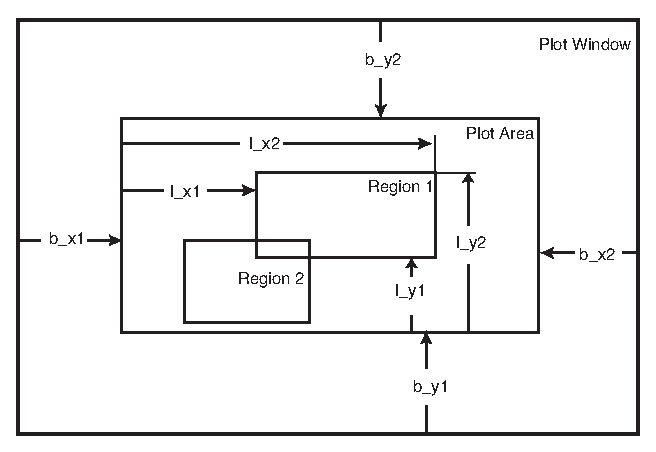
\includegraphics{plot_page.psfig}
  \caption{Regions define where on the plot page plots are placed.}
  \label{f:plot_page}
\end{figure}

Plotting is defined by an initialization file named
\vn{tao_plot.init}.  The first namelist block in the file has a block
name of \vn{tao_plot_page}. This block sets the size of the plot
window (also called the plot page) and defines the ``regions'' where
plots go. The syntax of this block is:
\index{tao_plot_page}    
\index{plot_page!size}
\index{plot_page!border}
\index{plot_page!text_height}
\index{plot_page!title}
\index{region!name}
\index{region!location}
\index{place}
\begin{example}
  &tao_plot_page
    plot_page%size        = <x_size>, <y_size>         ! size in POINTS 
    plot_page%border      = <b_x1>, <b_x2>, <b_y1>, <b_y2>, "<units>"
    plot_page%text_height = <text_height>              !height in POINTS
    plot_page%title(i)    = <string>, {<x>, <y>, "<justify>", "<units>"}
    region(i)%name        = "<region_name>"
    region(i)%location    = <l_x1>, <l_x2>, <l_y1>, <l_y2>  ! % plot area
    place(i)              = "<region>", "<template>"
  /
\end{example}
For example:
\begin{example}
  &tao_plot_page
    plot_page%size        = 700, 800           ! Points
    plot_page%border      = 0, 0, 0, 50, "POINTS"  
    plot_page%text_height = 12.0
    plot_page%title(1)    = "CESR Lattice"
    region(1)%name        = "top"
    region(1)%location    = 0.0, 1.0, 0.5, 1.0
    region(2)%name        = "bottom"
    region(2)%location    = 0.0, 1.0, 0.0, 0.5
    place(1)              = "top", "orbit"
    place(2)              = "bottom", "phase"
  /
\end{example}

\vn{plot_page%size} sets the horizontal and vertical size of the plot
window in \vn{POINTS} units (72 points = 1 inch. Roughly 1 point = 1
pixel). 

\vn{plot_page%border} sets a border around the edges of the
window. As shown in Figure~\ref{f:plot_page} \vn{b_x1}, \vn{b_x2} are
the right and left border widths and \vn{b_y1} and \vn{b_y2} are the
bottom and top border widths respectively.  The rectangle within this
border is called the plot area.

\vn{plot_page%title(i)} set the page title. There are two title areas 
(i = 1,2). If only the title string is given then the other variables 
are set to the defaults \vn{x} = 0.5, \vn{y} = 0.995, \vn{justify} = 
"CC" and \vn{units} = "%PAGE". See the quickplot documentation for 
the \vn{justify} variable syntax.

The plot area is divided up into rectangular regions where plots may
be placed (what defines a plot is discussed below).
\vn{region(i)%name} is the name of a region and my be any character
string. \vn{l_x1}, and \vn{l_x2} define the location of the left and
right edges of the region as a fraction of the plot area width
starting from the left edge of the plot area.  \vn{l_y1} and \vn{l_y2}
define the location of the bottom and top edges of the region as a
fraction of the height of the plot area with respect to the plot
area's bottom edge. Thus, in the above example, region 1 extends from
the left border of the plot area (\vn{region(1)%l_x1} = 0) to the
right border (\vn{region(1)%l_x2} = 0) and vertically from the center
(\vn{region(1)%l_y1} = 0.5) to the top edge (\vn{region(1)%l_x2} =
1.0). Regions may overlap any one can define as many regions as one
likes.

\vn{place(i)} determines the initial placement of plots.

%-----------------------------------------------------------------
\subsection{Templates}\index{Initialization!Plotting!Templates}

As shown in Figure~\ref{f:plot}, a ``plot'' is made up of a collection
of ``graphs'' and a graph consists of axes plus a set of ``curves''.
In the \vn{tao_plot.init} file there needs to be defined a set of
``template plots''. A template plot specifies the layout of a plot:
How the graphs are placed within a plot, what curves are associated
with what graphs, etc. When running \tao, the information in a
template plot may then be transfered to a region using the \vn{place}
command and this will produce a visible plot.

Template plots are defined using namelists with a name of
\vn{tao_template_graph}. The general syntax is:
\index{tao_template_plot}
\index{plot!name}
\index{plot!x}
\index{plot!x_axis_type}
\index{plot!ix_universe}
\index{plot!n_graph}
\index{plot!independent_graphs}
\begin{example}
  &tao_template_plot
    plot%name        = "<plot_name>"
    plot%x           = <qp_axis_struct>
    plot%x_axis_type = "<x_axis_type>"   ! "index" or "s". Default is "index".
    plot%ix_universe = <number> ! used for lat_layout plots
    plot%n_graph     = <n_graphs>
    plot%independent_graphs = <logical>  ! scale graph y-axis independently
  /
\end{example}
For example:
\begin{example}
  &tao_template_plot
    plot%name        = "orbit"
    plot%x%min       =   0
    plot%x%max       = 100
    plot%x%major_div = 10
    plot%x%label     = "Index"
    plot%n_graph     = 2
  /
\end{example}

\vn{plot%x} sets the properties of the horizontal axis. For more
information see the \vn{Quick Plot} documentation on the
\vn{qp_axis_struct}. The major components are
\index{qp_axis_struct!min}
\index{qp_axis_struct!max}
\index{qp_axis_struct!major_div}
\index{qp_axis_struct!minor_div}
\index{qp_axis_struct!label}
\begin{example}
  min        ! Left edge value.
  max        ! Right edge value.
  major_div  ! Number of major divisions. 
             !  Number of major tick marks is one less.
  minor_div  ! Number of minor divisions. 0 = auto choose.
  label      ! Axis label.
\end{example}

\vn{plot%name} is the name that is used with \tao commands to identify
the plot.  

\vn{plot%x_axis_type} sets what is plotted along the
\vn{x-axis}. Possibilities are:
\index{index}
\index{ele_index}
\index{s}
\begin{example}
    "index"      ! Data Index
    "ele_index"  ! Element lattice number index
    "s"          ! Longitudinal position in the lattice.
\end{example}

\vn{n_graph} sets the number of graphs associated with the plot and
each one needs a \vn{tao_template_graph} namelist to define it. These
namelists should be placed directly after their respective
\vn{tao_template_graph} namelists. The general format of the
\vn{tao_template_graph} namelist is:
\index{tao_template_graph}\index{graph!y}\index{curve!name}
\index{graph_index}\index{graph}\index{graph!name}\index{curve}
\index{graph!type}\index{graph!box}\index{graph!title}\index{graph!margin}
\index{graph!y2}\index{graph!n_curve}\index{graph!clip}\index{graph!who}
\index{curve!data_type}\index{curve!data_source}
\index{curve!x_axis_units_factor}\index{curve!y_axis_units_factor}
\index{curve!use_y2}\index{curve!line}\index{curve!ele_ref_name}
\index{curve!draw_line}\index{curve!draw_symbols}\index{curve!ix_universe}
\index{curve!symbol}\index{curve!symbol_every}\index{curve!convert}
\begin{example}
  &tao_template_graph
    graph_index           = <number>
    graph%name            = "<graph_name>"
    graph%type            = "<graph_type>"
    graph%box             = <ix>, <iy>, <ix_tot>, <iy_tot>
    graph%title           = "<label>''
    graph%margin          =  <ix1>, <ix2>, <iy1>, <iy2>, "<Units>"
    graph%y               = <qp_axis_struct>
    graph%y2              = <qp_axis_struct>
    graph%n_curve         = <number_of_curves>
    graph%clip            = <logical> ! Clip plot at grpah boundary. default = .true.
    graph%who(i)          = "<who_to_plot>", <sign>
    curve(i)%name         = "<curve_name>"
    curve(i)%data_type    = "<data_type>"
    curve(i)%data_source  = "<source_name>" !source for the data curve points
    curve(i)%x_axis_scale_factor = <factor> ! scale the x-axis by this.
    curve(i)%y_axis_scale_factor = <factor> ! scale the y-axis by this.
    curve(i)%use_y2       = <logical> 
    curve(i)%draw_line    = <logical>
    curve(i)%draw_symbols = <logical>
    curve(i)%ix_universe  = <universe_number> ! default = 0 => use viewed universe
    curve(i)%line         = <qp_line_struct>
    curve(i)%symbol       = <qp_symbol_struct>
    curve(i)%symbol_every = <integer>       ! plot symbol every # datums
    curve(i)%convert      = <Logical>
    curve(i)%draw_interpolated_curve = <Logical>
    curve(i)%ele_ref_name = "<element_name>"     ! reference element.
  /
\end{example}
For example:
\begin{example}
  &tao_template_graph
    graph_index           = 1
    graph%name            = "x"
    graph%type            = "data"
    graph%box             = 1, 1, 1, 2
    graph%title           = "Horizontal Orbit (mm)"
    graph%margin          =  60, 200, 30, 30, "POINTS"
    graph%y%label         = "X"
    graph%y%max           =  4
    graph%y%min           = -4
    graph%y%major_div     = 4
    graph%n_curve         = 1
    graph%who(1)          = "model", +1
    graph%who(2)          = "design", -1
    curve(1)%data_source  = 'data_array'
    curve(1)%data_type    = "orbit.x"
    curve(1)%units_factor = 1000
    curve(1)%use_y2       = .false.
  /
\end{example}

\vn{graph%name} and \vn{curve%name} define names to be used with
commands. The default names are just the letter \vn{g} or \vn{c} with
the index of the graph or
curve. Thus, in the example above, the name of the curve defaults to
\vn{c1} and it would be referred to as \vn{orbit.x.c1}.

\vn{graph%who(i)} sets what is plotted. In the above example, what will be
plotted is \vn{model - design}. Possible \vn{graph%who}
settings are:
\index{model}\index{design}\index{base}\index{meas}\index{ref}
\begin{example}
  "model"     ! model values.
  "design"    ! design values.
  "base"      ! Base values
  "meas"      ! data values.
  "ref"       ! reference data values.
\end{example}
The default, if \vn{graph%who} is not
specified, is for the graph will show \vn{model} values. 

\vn{graph%type} is the type of graph. \tao knows about the
following types:
\index{data}\index{lat_layout}\index{key_table}\index{phase_space}
\begin{example}
  "data"         ! Data plots (default) 
  "floor_plan"   ! A 2-dimentional birds-eye view of the machine.
  "key_table"    ! Key binding table for single mode.
  "lat_layout"   ! Schematic showing placement of the lattice elements.
  "phase_space"  ! Phase space plots
\end{example}
The \vn{key_table} is drawn with respect to the upper left hand corner
of the region in which it is placed.

\vn{graph%box} sets the layout of the box which the \vn{graph} is
placed in. For a definition of what a box is see the Quick Plot
documentation in the \bmad reference manual. In the above example the
graph divides the region into two vertically stacked boxes and places
itself into the bottom one. 

\index{data_array}\index{var_array}\index{calculation}
\index{curve!data_source}
The \vn{curve} structure is used to define the number and types of
curves to plot in each graph. \vn{curve%data_source} is the type of
information for the source of the data points. There are the following
types of data sources:
\begin{example}
  "data_array"       ! A d1_data array is the source of the curve points.
  "var_array"        ! A v1_var array is the source of the curve points.
  "calculation"      ! The curve points are computed directly from the lattice.
  "beam_calculation" ! The curve points are computed tracking a beam of particles.
\end{example}
With \vn{curve%data_source} set to \vn{data_array}, the values of the
curve points come from the \vn{d1_data} array structure named by
\vn{curve%data_type}. Thus in the above example the curve point values
are obtained from \vn{orbit.x} data. To be valid the data structure
named by \vn{curve%data_type} must be set up in an initialization
file. Similarly, \vn{var_array} indicates that the values of the curve
points come from a \vn{v1_var} array structure. \vn{calculation} means
that the curve data points are calculated from the lattice without
regard to any data structures. \vn{beam_calculation} is used when
tracking beams of particles or macroparticles. In this case the curve
points are calculated from the tracking. For example, with
\vn{curve%data_type} set to \vn{beta.x}, the setting of
\vn{curve%data_source} to \vn{calculation} gives the beta as
calculated from the lattice and \vn{beam_calculation} gives the beta
as calculated from the shape of the beam. 

For a curve with the \vn{curve%data_source} set to \vn{"data_array"} the
possible \vn{curve%data_type} values are the same as the possible
\vn{d1_data%type} values as given in \sref{s:data_types}. If the
\vn{curve%data_source} is \vn{"var_array"} then the possible
\vn{curve%data_type} values are any of the \vn{v1_var} names. This is
what points the curve to the proper data so there needs to be a
corresponding data or var type defined in the initialization file.  If
\vn{graph%type} is \vn{"phase_space"} then \vn{curve%data_source}
determines what planes are plotted. A plane is either:
\index{x}\index{p_x}\index{y}\index{p_y}\index{z}\index{p_z}
\begin{example}
  "x"
  "p_x"
  "y"
  "p_y"
  "z"
  "p_z"
\end{example}
For example:
\begin{example}
  curve%data_type = "x-p_x"  ! x-axis - y-axis
\end{example}
The dash \vn{-} is mandatory as the separator between the plane names. 

\vn{curve%convert} is a logical that is only used
with \vn{curve%data_name} = "coupling" and tells \tao to convert the
coupling data into cbar data before plotting.

\vn{curve%draw_symbols} determines whether a symbol is drawn at the
data points. The size, shape and color of the symbols is determined by
\vn{curve%symbol}.

\vn{curve%draw_line} determines whether a curve is drawn through the
data points. The thickness, style (solid, dashed, etc.), and color
is determined by \vn{curve%line}

%-----------------------------------------------------------------
\subsection{Lattice Layout}\index{Initialization!Lattice Layout}

A lattice layout template plot may be defined that draws the lattice
along a straight line with figures for the various elements.
The \vn{tao_template_plot} needed to define a lattice layout looks like:
\index{tao_template_plot}\index{plot!name}\index{plot!box_layout}
\index{plot!x!min}\index{plot!x!max}\index{plot!n_graph}
\index{tao_template_graph}\index{graph_index}\index{graph!name}
\index{graph!type}\index{graph!title}\index{graph!box}
\index{graph!ix_universe}\index{graph!margin}\index{graph!n_curve}
\begin{example}
  &tao_template_plot
    plot%name        = "<plot_name>"
    plot%box_layout  = <ix>, <iy> 
    plot%x%min       = <number>
    plot%x%max       = <number>
    plot%n_graph     = <number>
  /
  &tao_template_graph
    graph_index       = <number>
    graph%name        = <name>
    graph%type        = "lat_layout"
    graph%title       = "Layout Title"
    graph%box         = <ix>, <iy>
    graph%ix_universe = <integer> ! 0 => use currently viewd universe
    graph%margin      = <ix1>, <ix2>, <iy1>, <iy2>, "<Units>"
    graph%n_curve     = 0
  /
\end{example}
Example:
\begin{example}
  &tao_template_plot
    plot%name       = 'layout'
    plot%x%min      =   0
    plot%x%max      = 100
    plot%n_graph    = 1
  /

  &tao_template_graph
    graph_index       = 1
    graph%name        = 'u1'
    graph%type        = 'lat_layout'
    graph%this_box    = 1, 1
    graph%ix_universe = 1
    graph%margin      = 0.12, 0.12, 0.12, 0.12, '%BOX'
    graph%n_curve     = 0
  /
\end{example}

\index{element_shapes}
\index{shape}
With a \vn{graph%type} of \vn{lat_layout} or \vn{floor_plan}, 
the shapes to be drawn for the various lattice elements need to
be defined using an \vn{element_shapes} namelist whose syntax is:
\begin{example}
  &element_shapes 
    shape(i) = "<key>", "<name>", "<shape>", "<color>", 
                                      "<v_size>", "<print_Label>"
  /
\end{example}
For Example:                 
\begin{example}
  &element_shapes
    shape(1) = "Quadrupole", "Q*",      "Box",  "Red",      30,   T 
    shape(2) = "Quadrupole", "*",       "XBox", "Red",      30,   F 
    shape(3) = "SBend",      "*",       "Box",  "Blue",     15 
    shape(4) = "Wiggler",    "*",       "XBox", "Green",    20 
  /
\end{example}

A figure is drawn for each element in the lattice that matches a
shape. A Match is made if the type of element matches the shape
\vn{<key>} and the name of the element matches the shape
\vn{<name>}. The wildcard ``*'' may be used to denote any number of
characters. Thus, in the example above, \vn{shape(1)} will match to
all quadrupoles whose name begins with ``Q'' and \vn{shape(2)} will
match all quadrupoles. If an element matches more than one shape the
first shape matched will be used. \vn{<shape>} is the shape of the
figure drawn. Valid Shapes are:
\index{box}\index{xbox}
\begin{example}
  "BOX"             -- Rectangular box
  "XBOX"            -- Rectangular box with an x through it.
  "VAR_BOX"         -- Rectangular box with variable height. 
                        The box is symmetric about the center line.
  "ASYM_VAR_BOX"    -- Like VAR_BOX but is not symmetric about the center line. 
\end{example}
The height of a \vn{VAR_HEIGHT_BOX} is proportional to the element
strength. For example, for a quadrupole the height is proportional to
the \vn{K1} focusing strength. Not all elements can be used with a
\vn{VAR_HEIGHT_BOX}.

\vn{<color>} is the color of the shape. Good colors to use are:
\index{black}\index{Red}\index{orange}\index{magenta}\index{yellow}
\index{green}\index{cyan}\index{blue}\index{purple}
\begin{example}
  "BLACK"
  "RED"
  "ORANGE"
  "MAGENTA"
  "YELLOW"
  "GREEN"
  "CYAN"
  "BLUE"
  "PURPLE"
\end{example}
\vn{<v_size} is the vertical size of the shape in points (72 points =
1 inch). Finally \vn{<print_label>} is a logical indicating whether
the element name is to be printed underneath the figure.



%-----------------------------------------------------------------
\section{Initializing Key Bindings for Single Mode}\index{Initialization!Key Bindings}
\label{s:init_single} 

For single mode the bindings of variables to keys is defined with a
\vn{key_bindings} namelist. There is a maximum of 500 key bindings.
The syntax is:
\index{key_bindings}
\index{key}
\begin{example}
  &key_bindings
    key(i) = <ele_name> <attrib_name> <delta> <universe> 
          <small_step> <low_lim> <high_lim> <weight> <good_opt> <merit_type>
  /
\end{example}
For example:
\begin{example}
  &key_bindings
  key(1) = "Q1"   "K1"    0.01 "U:*" 1e-5  -10  10  10  T
  key(2) = "DRFT" "L"     0.1  "U:1" 1e-3    0   3   1  F
  key(3) = "Q3"   "TILT"  0.01 "U:2" 1e-5   -1   1   3  T "target"
  /  
\end{example}
For the \vn{i}\Th key \vn{<ele_name>} is the name of a lattice element
in universe \vn{<universe>} and \vn{<attrib_name>} is the attribute to
be varied. If \vn{<universe>} is ``0'' then the key will vary elements
in all universes. \vn{<delta>} is the change in value when the
appropriate key is depressed. \vn{<small_step>} establishes what a 
``small'' variation of the variable is. 

\vn{merit_type} sets the variable merit is calculated. See
\sref{s:init_var} for more details. the \vn{global%default_key_merit_type} 
sets the default \vn{merit_type}.

If \vn{merit_type} is \vn{"limit"} then \vn{<low_lim>} and
\vn{<high_lim>} establish limits and if the value of the variable goes
outside these limits then the contribution to the merit function is
given by
\index{merit function}
\begin{example}
  merit = <weight> * (var_value - <high_lim>)^2  ! For var_value > <high_lim>
  merit = <weight> * (<low_lim> - var_value)^2   ! Fro <low_lim> > var_value
\end{example}

\chapter{Tao Line Mode Commands}
\label{c:command}

\tao has two \vn{modes} for entering commands. In \vn{Line Mode},
described in this chapter, \tao waits until the \vn{return} key is
depressed to execute a command. That is, a command consists of a
single line of input. Conversely, \vn{Single Mode}, which is described
in Chapter~\sref{c:single}, interprets each keystroke as a
command. Single Mode is useful for quickly varying parameters to see
how they affect a lattice but the number of commands in Single Mode is
limited.

Commands are case sensitive. The list of commands is shown in
Table~\ref{t:commands}.\index{Commands!Command List} Multiple commands
may be entered on one line using the ``;'' character as a separator.

%% command_table -----------------------------------------------------

\begin{table}[h]
\centering {\tt
\begin{tabular}{|l|l||l|l|} \hline
  {\it Command} & {\it Section}  & {\it Command} & {\it Section}  \\ \hline
  alias      & \sref{s:alias}    & read         & \sref{s:read}     \\ \hline
  call       & \sref{s:call}     & restore      & \sref{s:restore}  \\ \hline 
  change     & \sref{s:change}   & reinitialize & \sref{s:reinit}   \\ \hline 
  clip       & \sref{s:clip}     & run          & \sref{s:run}      \\ \hline 
  derivative & \sref{s:deriv}    & scale        & \sref{s:scale}    \\ \hline 
  end-file   & \sref{s:end-file} & set          & \sref{s:set}      \\ \hline  
  exit       & \sref{s:exit}     & show         & \sref{s:show}     \\ \hline 
  flatten    & \sref{s:flatten}  & single-mode  & \sref{s:sing}     \\ \hline 
  help       & \sref{s:help}     & spawn        & \sref{s:spawn}    \\ \hline 
  history    & \sref{s:history}  & use          & \sref{s:use}      \\ \hline 
  misalign   & \sref{s:misalign} & veto         & \sref{s:veto}     \\ \hline 
  output     & \sref{s:output}   & view         & \sref{s:view}     \\ \hline 
  place      & \sref{s:place}    & x-axis       & \sref{s:x-axis}   \\ \hline 
  plot       & \sref{s:plot}     & x-scale      & \sref{s:x-scale}  \\ \hline 
  quit       & \sref{s:quit}     & xy-scale     & \sref{s:xy-scale} \\ \hline
\end{tabular}}
\caption{Table of \tao commands.}
\label{t:commands}
\end{table}

%% Marker: "help" will not display anything after this  -----------

\index{Arithmetic expressions} 
The \tao command prompt parser can handle arithmetic expressions. 
Arithmetic expressions can be used in a place where a real value is required.
The standard operators are defined: \hfil\break
\hspace*{0.15in}
\begin{tabular}{ll}
  $a + b$           & Addition        \\
  $a - b$           & Subtraction     \\
  $a \, \ast \, b$  & Multiplication  \\
  $a \; / \; b$     & Division        \\
  $a \, \land \, b$ & Exponentiation  \\
\end{tabular} \newline
The following intrinsic functions are also recognized: \hfil\break
\index{Intrinsic functions}
\hspace*{0.15in}
\begin{tabular}{ll}
  \vn{sqrt}(x)      & Square Root    \\
  \vn{log}(x)       & Logarithm      \\
  \vn{exp}(x)       & Exponential    \\
  \vn{sin}(x)       & Sine           \\
  \vn{cos}(x)       & Cosine         \\
  \vn{tan}(x)       & Tangent        \\
  \vn{asin}(x)      & Arc sine       \\
  \vn{acos}(x)      & Arc cosine     \\
  \vn{atan}(x)      & Arc Tangent    \\
  \vn{abs}(x)       & Absolute Value \\
  \vn{ran}()        & Random number between 0 and 1 \\
  \vn{ran_gauss}()  & Gaussian distributed random number with unit RMS \\
\end{tabular} \newline
Both \vn{ran} and \vn{ran_gauss} use a seeded random number generator. 
Setting the seed is described in Section~\sref{s:globals}.

For a description of \vn{single mode} commands see
Chapter~\ref{c:single}. To put \tao into \vn{single mode} use the
\vn{single_mode} command. 

\vfil
\break

%% alias --------------------------------------------------------------
\section{alias}\index{Commands!alias}
\label{s:alias}

Format: 
\begin{example}
  alias \{<alias_name> <string>\}
\end{example}

\vskip 0.2in

\vn{Alias} is like Unix aliases and allows the defining of alias
commands. Using the \vn{alias} command without any arguments results
in a printout of the aliases that have been defined. When using an
alias up to 9 arguments may be substituted in the \vn{<string>}. The
i\Th argument is substituted in place of the sub-string ``[[i]]''.
arguments that do not have a corresponding ``[[i]]'' are placed at the end
of \vn{<string>}

Examples:
\begin{example}
    alias xyzzy plot [[1]] model  ! Define xyzzy
    alias                         ! Show all aliases
    xyzzy top                     ! Use an alias
    plot top model                ! Equivalent to "xyzzy top"
    xyzzy top abc                 ! Equivalent to "plot top model abc"
\end{example}
In the above example ``xyzzy'' is the alias for the string ``plot [[1]]
model''.  When the command xyzzy is used ``top'' is substituted
for ``[[1]]'' in the string.

%% call --------------------------------------------------------------
\section{call}\index{Commands!call}
\label{s:call}

Format: 
\begin{example}
  call <filename> \{<arg_list>\}  \Strut
\end{example}

\vskip 0.2in 
\vn{call} opens a command file and executes the commands
in it.  \tao first looks in the current directory for the file. If not
found \tao will look in the directory pointed to by the
\vn{TAO_COMMAND_DIR} directory.  Up to 9 arguments may be passed to
the command file. The i\Th argument is substituted in place of the
string ``[[i]]'' in the file. Nesting of command files (command files
calling other command files) is allowed. There is no limit to the
number of nested files.

Do loops are allowed with the following syntax:
\begin{example}
  do <var> <begin> <end> <step> 
    ...
    tao command [[<var>]]
    ...
  enddo
\end{example}
\vn{<var>} can be any character string up to 10 characters long.
The \vn{<var>} can be used as a variable in the loop body but must be
bracketed.  The step size can be any integer positive or negative but not zero.
Nested loops are allowed. Command files can be called within do loops.

Examples:
\begin{example}
    call my_cmd_file abc def 
\end{example}
In the above example the argument ``abc'' is substituted for any
``[[1]]'' appearing the file and ``def'' is substituted for any
``[[2]]''.
\Newline

\begin{example}
  do i 1 100
    call set_quad_misalignment [[i]] ! command file to misalign quadrupoles
    zero_quad 1e-5*2^([[i]]-1) ! Some user supplied command to zero quad number [[i]]
  enddo
\end{example}

%% change --------------------------------------------------------------
\section{change}\index{Commands!change}
\label{s:change}

Format:
\begin{example}
  change ele <name_or_number> <attribute> <number>
  change var <name> <locations> <number>
  change beam_start <coordinate> <number>
\end{example}

\vskip 0.2in 
\vn{change} changes element attribute values or variable
values in the \vn{model} lattice. To set, say, datum values, etc. use
the \vn{set} command.

Generally \vn{<number>} is added to the existing value of the
attribute or variable. That is:
\begin{example}
  final_value = initial_value + <number>
\end{example}
If "@" is prepended to \vn{<number>} then just the value of
\vn{<number>} is used to set the value
\begin{example}
  final_value = <number>
\end{example}
If "d" is prepended to \vn{<number>} then the value relative to the design
value is used:
\begin{example}
  final_value = design_value + <number>
\end{example}

For linear lattices, \vn{change beam_start <coordinate> <number>} 
can be use to vary the starting coordinates where \vn{<coordinate>} is one of: 
\begin{example}
  (x, p_x, y, p_y, z, p_z)
\end{example}
For circular lattices only the \vn{p_z} component is applicable. 
Also for linear lattices, \vn{change ele beginning <twiss>} can be used to
vary the starting Twiss parameters where \vn{<twiss>} is one of:  
\begin{example}
  beta_a, beta_b, alpha_a, alpha_b 
  eta_a, eta_b,etap_a, etap_b    
\end{example}

Examples:
\begin{example}
  change ele 124 x_offset  0.1     ! Offset element #124 by 0.1
  change ele q02w k1 d 1.2e-2      ! set the k1 strength of q02w relative to the design
  change var steering[34:36] @1e-3 ! set the steering strength #34-36 to 0.001
  change var steering[*] @0.0      ! set all steering strengths to 0.0
  change beam_start x @0.001       ! set beginning x position to 1 mm
\end{example}


%% clip --------------------------------------------------------------
\section{clip}\index{Commands!clip}
\label{s:clip}

Format:
\begin{example}
  clip \{<where> <limit1> <limit2>\}
\end{example}

\vskip 0.2in 
\vn{clip} vetoes data points for optimizing. If points are vetoed and
either measured or reference data is being plotted then the points
clipped will no longer be plotted. The points vetoed are those points
whose $y$ values are outside a certain range defined by \vn{<limit1>}
\vn{<limit2>}. If neither \vn{<limit1>} nor \vn{<limit2>} is present
then the clip range is taken to be outside the graph minimum and
maximum $y$--axis values. If only \vn{<limit1>} is present then the
clip range is outside the range from -\vn{<limit1>} to
+\vn{<limit1>}. If both are present than the range is from
\vn{<limit1>} to \vn{<limit2>}.  The graphs that are clipped is
determined by the \vn{<where>} switch.  If \vn{<where>} is not present
all graphs are scaled.

Examples
\begin{example}
  clip top.x -3  7  ! clip the x graph in the top region
  clip bottom       ! clip the graphs in the bottom region
\end{example}

%% end-file --------------------------------------------------------------
\section{end-file}
\label{s:end-file}
\index{Commands!end-file}

The \vn{end-file} is used in command files (\sref{s:call}) to signal
the end of the file. Everything an \vn{end-file} command is
ignored. An \vn{end-file} command entered at the command line will
simply generate an error message.

%% exit --------------------------------------------------------------
\section{exit}\index{Commands!exit}
\label{s:exit}

Format:
\begin{example}
  exit
\end{example}

\vskip 0.2in
\vn{Exit} exits the program. Same as \vn{Quit}.

%% derivative --------------------------------------------------------------
\section{derivative}\index{Commands!derivative}
\label{s:deriv}

Format:
\begin{example}
  derivative
\end{example}

\vskip 0.2in 
\vn{Derivative} calculates the \vn{dModel_Data/dVar} derivative
matrix needed for the \vn{lm} optimizer.

%% flatten --------------------------------------------------------------
\section{flatten}\index{Commands!flatten}
\label{s:flatten}

Format:
\begin{example}
  flatten <optimizer>
\end{example}

\vskip 0.2in
\vn{Flatten} runs the optimizer to minimize the merit function. This is the 
same as \vn{run}. See the \vn{run} command for more details.

%% help --------------------------------------------------------------
\section{help}\index{Commands!help}
\label{s:help}

Format:
\begin{example}
  help <command>
\end{example}

\vskip 0.2in 
\vn{Help} gives help on \tao commands. The environmental
variable \vn{TAO_DIR} must be defined so \tao can find any help files.

Examples:
\begin{example}
  help run   ! Gives help on the run command
\end{example}

%% history --------------------------------------------------------------
\section{history}\index{Commands!history}
\label{s:history}

Format:
\begin{example}
  history           ! Print the command history.
  history <number>  ! Re-execute a command by number.
  history <string>  ! Re-execute last command that begins with <string>.
\end{example}

\vskip 0.2in
Every \tao command entered is recorded in a ``history stack'' and
these commands can be viewed and reinvoked as needed. 

Examples
\begin{example}
  history 34   ! Re-execute command number 34.
  history set  ! Re-execute last set command.  
\end{example}

%% misalign --------------------------------------------------------------
\section{misalign}\index{Command!misalign}
\label{s:misalign}

Format:
\begin{example}
   misalign <wrt> <ele_type> <locations> <ele_attrib> <misalign_value>
\end{example}

\vskip 0.2in
Misaligns a set of elements of type \vn{<ele_type>} at lattice
locations \vn{<locations>}.  The element attribute \vn{<ele_attrib>}
is ``misaligned'' by the rms value \vn{<misalign_value>} with respect
to the setting of \vn{<wrt>}. Any element attribute can be misaligned
provided the attribute is free to vary.

If \vn{<ele_type>} begins with "*@" then choose all universes. If
\vn{<ele_type>} begin with "n@" then choose universe n. Otherwise the
viewed universe is used.

\vn{<locations>} is a range of lattice indices in the form
\vn{nnn:mmm} or the work \vn{ALL}. Only elements of type
\vn{<ele_type>} will be misaligned within the range.

If \vn{<misalign_value>} is prepended by 'x' then the misalignment value will be
a relative misalignment with respect to the \vn{<wrt>} value. Otherwise, it's an 
absolute rms value about the \vn{<wrt>} value.

In the special case where sbend strengths are misaligned then use
\vn{<ele_attrib> = g_err}. However, if a relative error is specified it will be 
relative to 'g'.

The possible values of \vn{<wrt>} are:
\begin{example}
  wrt_model          ! Misalign about the current model value
  wrt_design         ! Misalign about the design value
  wrt_survey         ! Misalign about the zero value
\end{example}

Examples
\begin{example}
   ! The following will misalign all quadrupole vertical positions in the viewed
   ! universe within the lattice element range 100:250 with respect to the zero 
   ! value by 300 microns
  misalign wrt_survey quadrupole 100:250 y_offset 300e-6
   ! The following will misalign all quadrupole strengths in all universes for
   ! the entire lattice with respect to the design value by 1%.
  misalign wrt_design *@quadrupole ALL k1 x0.01
\end{example}

%% output --------------------------------------------------------------
\section{output}\index{Commands!output}
\label{s:output}

Format:
\begin{example}
  output bmad_lattice \{<file_name>\}       ! Write a Bmad lattice file of the model
  output beam \{-ascii\} \{-at <element_name_or_index>\} \{<file_name>\} 
                                          ! Write beam distribution data.
  output curve <curve_name> \{<file_name>\} ! Write the curve data
  output derivative_matrix \{file_name\}    ! Write the \vn{dModel_Data/dVar} matrix.
  output digested \{<file_name>\}     ! Write a digested Bmad lattice file of the model.
  output gif \{<file_name>\}          ! create a gif file of the plot window.
  output hard                       ! Print the plot window to a printer.
  output hard-l                     ! Like "hard" except use landscape orientation. 
  output mad_lattice \{<file_name>\}  ! Write a Mad lattice file of the model
  output ps \{<file_name>\}           ! Create a postscript file of the plot window.
  output ps-l \{<file_name>\}         ! Like "ps" except use landscape orientation.
  output var \{<file_name>\}          ! Write a Bmad file of variable values.
\end{example}

\vskip 0.2in 
The \vn{output} command creates various files. If
\vn{<file_name>} is not given then the defaults are:
\begin{example}
  Command                         Default File Name
  ------------------              ------------------
  output bmad_lattice             lat_#.bmad
  output beam                     beam_#.dat
  output curve                    curve
  output derivative_mat           derivative_matrix.dat              
  output digested                 digested8_lat_universe_#.bmad
  output gif                      tao.gif
  output mad_lattice              lat_#.mad
  output ps                       tao.ps
  output var                      global%var_out_file
\end{example}
where \vn{\#} is replaced by the universe number. \vn{output
curve} will produce two or three files: 
\begin{example}
  <file_name>.symbol_dat    ! Symbol coordinates file
  <file_name>.line_dat      ! Curve coords.
  <file_name>.particle_dat  ! Particle data file
\end{example}
The particle data file is only produced if particle
data is associated with the curve.
The curve coordinates are the the set of points that are used to draw the
(possibly smooth) curve through the symbols.

\vn{output beam} will create a file of the particle positions when
beam tracking is being used. If the switch \vn{-at} is present then
only the particle positions at the given element are written. 
Otherwise the positions at all elements will be written. The
\vn{-ascii} switch is for writing text files. The default is to write
with a compressed binary format.  Note: Beam files can be used to
initialize \tao (\sref{s:command_line}). 

Note: PGPLOT does a poor job producing gif files so consider
making a postscript file instead and using a ps to gif converter.

%% place --------------------------------------------------------------
\section{place}\index{Commands!place}
\label{s:place}

Format:
\begin{example}
  place <region> <template>
  place <region> none
\end{example}

\vskip 0.2in 
The \vn{place} command is used to associate a \vn{<template>} plot
with a \vn{<region>} and thus create a visible plot in that region. To
erase a plot from a region use the \vn{none} switch. Notice that by
using multiple \vn{place} commands a \vn{template} can be associated
with more than one region.

Examples:
\begin{example}
  place top orbit  ! place the orbit template in the top region
  place top none   ! erase any plots in the top region
\end{example}

%% plot --------------------------------------------------------------
\section{plot}\index{Commands!plot}
\label{s:plot}

Format:
\begin{example}
  plot <region> <who>
\end{example}

\vskip 0.2in 
The \vn{plot} command is used to determine who is plotted
in the graphs of a given region. Use a ``-'' for baselines. 

Examples:
\begin{example}
  plot bottom model - design       ! Plot model - design in the bottom region
  plot top meas - model + design - ref 
\end{example}

%% quit --------------------------------------------------------------
\section{quit}\index{Commands!quit}
\label{s:quit}

Format:
\begin{example}
  quit
\end{example}

\vskip 0.2in
\vn{Quit} exits the program. Same as \vn{exit}.

%% read --------------------------------------------------------------
\section{read}\index{Commands!read}
\label{s:read}

Format:
\begin{example}
  read lattice <file_name>
\end{example}

\vskip 0.2in 
The \vn{read} command is used to modify the currently
viewed \vn{model} lattice. For example, with the appropriate file,
the \vn{read} command can be used to misalign the lattice
elements. The input file must be in Bmad standard lattice format.

%% restore --------------------------------------------------------------
\section{restore}\index{Commands!restore}
\label{s:restore}

Format:
\begin{example}
  restore data  <data_name> <locations>
  restore var <var_name> <locations>
\end{example}

\vskip 0.2in 
The \vn{restore} command cancels data or variable
vetoes. See also the \vn{use}
and \vn{veto} commands.

Examples:
\begin{example}
  restore data orbit.x[23,34:56]   ! un-veto orbit.x 23 and 34 through 56.
  restore data orbit.x[23,34:56:2] ! un-veto orbit.x 23 and even datums between 34 
                                   !                                          and 56
  restore data *@orbit[34]         ! un-veto orbit data in all universes.
  restore var quad_k1[67]          ! un-veto variable
\end{example}

%% reinitialize -------------------------------------------------------
\section{reinitialize}\index{Commands!reinitialize}
\label{s:reinit}

Format:
\begin{example}
  reinitialize beam
  reinitialize data
  reinitialize tao \{-init <tao_input_file>\} 
                       \{-beam <beam_input_file>\} \{-lat <lattice_file>\}
\end{example}

\vskip 0.2in 
\vn{reinitialize beam} reinitializes the beam at the start of the
lattice.  That is, a new random distribution is generated. This also
reinitializes the model data.

\vn{reinitialize data} forces a recalculation of the model data.
Normally, a recalculation is done automatically when any lattice
parameter is changed so this command is generally only useful for
debugging purposes.

\vn{reinitializes tao} reinitializes \tao. This can be useful to reset
everything to initial conditions or to perform analysis with more than
one initialization file.  See section \sref{s:command_line} for
details on the arguments.  If there are no arguments, the
\vn{reinitialize} command uses the same arguments that were used in
the last \vn{reinitialize} command, or, if this is the first
reinitialization, what was used to start \tao. If there are arguments,
The defaults will be used.  The default \vn{<init_file>} is what was
used with the last reinitialization or, if this is the first
reinitialization, what was used at startup.

Examples:
\begin{example}
  reinit tao                         ! Reinit using previous arguments
  reinit tao -init tao_special.init  ! Reinitializes \tao with the initialization file 
                                     !   tao_special.init
\end{example}


%% run --------------------------------------------------------------
\section{run}\index{Commands!run}
\label{s:run}

Format:
\begin{example}
  run \{<optimizer>\}
\end{example}

\index{de!optimizer}\index{lm!optimizer}
\vskip 0.2in 
The \vn{run} command runs an optimizer. If \vn{<optimizer>} is not
given then the default optimizer is used. To stop the optimizer before
it is finished press the period ``.''  key. If you want the optimizer
to run forever run the optimizer in \vn{single mode}. Valid optimizers
are:
\begin{example}
  lm            ! Levenburg-Marquardt from Numerical Recipes 
  lmdif         ! Levenburg-Marquardt 
  de            ! Differential Evolution
\end{example}

Examples:
\begin{example}
  run 
  run de
\end{example}

%% scale --------------------------------------------------------------
\section{scale}\index{Commands!scale}
\label{s:scale}

Format:
\begin{example}
  scale \{-axis\} \{<where> <value1> <value2>\}
\end{example}

\vskip 0.2in 
\vn{scale} adjusts the vertical scale of graphs. If neither
\vn{<value1>} nor \vn{<value2>} is present then the scale is adjusted
so that all the data points are within the graph region.  If only
\vn{<value1>} is present then the scale is taken to be from
-\vn{<value1>} to +\vn{<value1>}. If both are present than the scale
is from \vn{<value1>} to \vn{<value2>}.  The graphs that are scaled is
determined by the \vn{<where>} switch. If \vn{<where>} is not present
or \vn{<where>} is \vn{all} then all graphs are scaled.

A graph can have a \vn{y2} (left) axis scale that is separate from the \vn{y} (right) 
axis. Normally, the \vn{scale} command will scale both axes.  Scaling of just one of these
axes can be achieved by using the \vn{/axis} switch. Possible values for \vn{/axis} are:
\begin{example}
  -y                 ! Scale only the y axis.
  -y2                ! Scale only the y2 axis.
\end{example}

Examples:
\begin{example}
  scale top.x -3  7  ! Scale the x graph in the top region
  scale -y2 top.x    ! Scale only the y2 axis of the top.x graph.
  scale bottom       ! Scale the graphs in the bottom region
  scale              ! Scale everything
\end{example}


%% set --------------------------------------------------------------
\section{set}\index{Commands!set}
\label{s:set}

Format:
\begin{example}
  set curve <curve> <component> = <value>
  set data <data_name>|<component> = <value>
  set global <component> = <value>
  set graph <graph> <component> = <value>
  set lattice <component> = <value>
  set plot_page <component> = <value1> \{<value2>\}
  set universe <universe> <on/off> <recalculate>
  set var <var_name>|<component> = <value>
\end{example}

\vskip 0.2in 
The \vn{set} command is used to set values for datums,
variables, etc.  For setting element attributes in the \vn{model}
lattice use the \vn{change} command.

To apply a set to all data or variable classes use ``*''
in place of \vn{<data_name>} or \vn{var_name}.

For \vn{set curve}, the \vn{<component>}s that can be set are:
\begin{example}
  ele_ref_name   ! Name of reference element
  ix_ele_ref     ! Index of reference element
  ix_universe    ! Universe index.
  symbol_every   ! Symbol skip number.
\end{example}

For \vn{set data}, the \vn{<component>}s that can be set are:
\begin{example}
  base        ! Base model value
  design      ! Design model value
  meas        ! Measured data value.
  ref         ! Reference data value.
  weight      ! Weight for the merit function.
  exists      ! Valid datum for computations?
  good_meas   ! A valid measurement has been taken?
  good_ref    ! A valid reference measurement has been taken?
  good_opt    ! Good for using in the merit function for optimization?
  good_plot   ! Good for using in a plot?
  good_user   ! This is what is set by the use, veto, and restore commands.
  merit_type  ! How merit contribution is calculated.
\end{example}
Besides a numeric value \vn{<value>} can be any of the above along with:
\begin{example}
  meas        ! Measured data value.
\end{example}
\vskip 0.2in

For \vn{set graph}, the \vn{component}s that can be set are:
\begin{example}
  who(<n>)    = <string>
  who(<n>)    = <string>, <integer>
  clip        = <logical>
  ix_universe = <number>
  margin%x1   = <number>
  margin%x2   = <number>
  margin%y1   = <number>
  margin%y2   = <number>
\end{example}
\vskip 0.2in

For \vn{set global}, the \vn{show global} will give a list of the
\vn{<component>}s that can be set are
\vskip 0.2in

For \vn{set lattice}, the \vn{<component>}s that can be set are:
\begin{example}
  model      ! Model lattice value.
  base       ! Base lattice value
\end{example}
\vn{<value>} can be:
\begin{example}
  model       ! model lattice value.
  base        ! base lattice value.
  design      ! design lattice value
\end{example}
\vskip 0.2in

For \vn{set plot_page}, the \vn{<component>}s that can be set are:
\begin{example}
  title        = <string>          ! Set the plot title text
  subtitle     = <string>          ! Set the subtitle text
  subtitle_loc = <number> <number> ! Set the subtitle location (\%PAGE)
\end{example}
The \vn{subtitle_loc} component can be used to place the subtitle anywhere on
the plot page. This can be useful for referencing a noteworthy part of a graph
data.
\vskip 0.2in

For \vn{set var}, the \vn{<component>}s that can be set are:
\begin{example}
  model       ! Model lattice value.
  base        ! Base model value
  design      ! Design model value
  meas        ! Value at the time of a measurement.
  ref         ! Value at the time of a reference measurement.
  weight      ! Weight for the merit function.
  exists      ! Does this variable actually correspond to something?
  good_var    ! The optimizer can be allowed to vary it
  good_opt    ! Good for using in the merit function for optimization?
  good_plot   ! Good for using in a plot?
  good_user   ! This is what is set by the use, veto, and restore commands.
  step        ! Sets what a "small" variation of the variable is.
  merit_type  ! How merit contribution is calculated.
\end{example}
\vskip 0.2in

\vn{set universe} will turn the specified universe on or off. Turning
a universe off is useful to speed up lattice calculations when this
universe is not being used. Or, if many changes are to be performed to
a universe and there is no need to do any lattice calculations between
commands then turning off all universes will speed things up. To turn off 
the currently viewed universe use the command \vn{set universe 0 off}. 
To turn off all universes use the command \vn{set universe * off}. 
This flag only affects the lattice calculation. 
Issuing \vn{change, use, veto,} etc...  commands to a turned off universe
will still affect the
universe, however any lattice calculations will not be performed until
the universe is turned back on.  To recalculate the turned on lattices
when issuing a \vn{set universe} command then use \vn{set universe
<universe> <on/off> recalc}. Otherwise, no lattice calculation will
be performed until an appropriate command is called afterwards.  If
optimizing while one or more universes are turned off then the
variables associated with that universe will still be included in the
merit function but not the data for that universe. The variables will
still vary in the turned off universe.

Examples:
\begin{example}
  set data *|ref = *|meas               ! Set ref data = measured in current universe.
  set data 2@orbit.x|base = 2@orbit.x|model 
                                        ! Set the base orbit.x in universe 2 to model
  set graph orbit.x who(1) = model      ! Plot the model orbit in the graph
  set graph orbit.x who(2) = design, -1 ! With the previous line: Plot model - design 
  set var quad\_k1 weight = 0.1         ! Set quad\_k1 weights. 
  set lattice *@*|model = *@*|design    ! Reset model to the design in all universes
\end{example}

%% show --------------------------------------------------------------
\section{show}\index{Commands!show}
\label{s:show}

The \vn{show} command has an optional argument to write the results to a file.
The format for this is:
\begin{example}
  show -write <file_name> <rest_of_the_command>
\end{example}

Format:
\begin{example}
  show alias 
  show beam \{<element_index>\}
  show constraints
  show curve <curve_name> \{-symbol\} \{-line\}
  show data \{<data_name>\} 
  show element <name>
  show global
  show graph <graph_name>
  show hom
  show lattice \{-middle\} \{-custom <file_name>\} \{-s\} \{-elements <name>\} \{<location_range>\}
  show optimizer
  show opt_vars
  show particle lost
  show particle <particle_index>
  show plot
  show plot \{<template_plot_name>\}
  show plot \{<plot_region_name>\}
  show taylor <ele_name>
  show top10
  show universe \{universe_number\}
  show variable \{<var_name> <locations>\}
  show variable <universe_number>@
  show -write <file_name> ...
\end{example}

\vskip 0.2in 
\vn{Show} is used to display various information about
the state of \tao. 

\vn{Show -write} writes to a file as well as printing the information
at the terminal. Results are appended to the output file when \vn{show
-write} is used multiple times. If separate files are desired then if
\vn{global%write_file} has a \vn{*} character in it, a three digit
number is substituted for the \vn{*}. The value of the number starts
at \vn{001} and increases by 1 each time \vn{show -write} is used.

\begin{description}
  \item[show alias]
Shows a list of defined aliases. See the \vn{alias} command for more
details.

  \item[show beam]
If \vn{<element_index>} is absent, \vn{show beam} shows parameters 
used with beam tracking including the number of particles in a bunch, etc.
If \vn{<element_index>} is present, \vn{show beam} will show 
beam prameters at the selected element. Also see \vn{show particle}.

  \item[show constraints]
Lists data and variable constraints.

  \item[show curve]
Show information on a particular curve of a particular plot. See
\sref{s:plotting} for the syntax on plot, graph, and curve names.  Use
\vn{show plot} to get a list of plot names. The \vn{-symbol} switch
will additionally print the (x,y) points for the symbol placement and
the \vn{-line} switch will print the (x,y) points used to draw the
``smooth'' curve in between the symbols.

  \item[show data]
Shows data information. If \vn{<data_name>} and \vn{<locations>} are not
present shown is a list of \vn{d2_data} names.

  \item[show element]
This shows information on lattice elements. \vn{name} is in
\vn{Class:Name} syntax as explained in \sref{s:class:name}. If
\vn{<name>} contains a wild card or a class name then a list of
elements that match the name are shown. If no wild--card or class name
is present then information about the element whose name matches
\vn{<name>} is shown. All data types associated with the element
will also be listed. \vn{<name>} is a number $n$ then the $n$\Th
element in the lattice list will be shown.

\vn{show element} does not show the Taylor map associated with an element
even if it has one. To see this map use the \vn{show taylor}
command. Additionally, by default the wiggler terms of a \vn{map_type}
\vn{wiggler} element will not be printed. To change this use the command:
\vn{set global show_ele_wig_terms = T}.

  \item[show global]
Shows information on the global parameter structure (\sref{s:globals}).

  \item[show graph]
Show information on a particular graph of a particular plot. See
\sref{s:plotting} for the syntax on plot, graph, and curve names.
Use \vn{show plot} to get a list of plot names.

  \item[show hom]
Shows long--rang higher order mode information for linac accelerating
cavities.

  \item[show lattice]
Shows Twiss and orbit data for the \vn{model} lattice at the specified
element locations. The default is to show the parameters at the exit
end of the elements. To show the parameters in the middle use the
\vn{-middle} switch.

The locations to show can either be specified using the \vn{-elements}
switch, or by specifying a longitudinal position range with \vn{-s},
or (the default) by specifying a range of element indexes.  The
\vn{-elements} switch is used specify elements using a \vn{class:name}
format (\sref{s:class:name}). For example:
\begin{example}
  show lat -ele marker:bpm*
\end{example}
This will show the parameters at all marker elements whose name begin
with \vn{"bpm"}. 

Alternatively, a range of elements can be specified using the element
index or the element's longitudinal position with a \vn{":"} being
used to separate the index. For example
\begin{example}  
  Show lat  45:76, 101, 106    ! Show element #45 through #76 and 101 and 106.
  show lat -s  23.9:55.3       ! Show elements whose position is between 
                               !   23.9 meters and 55.3 meters .
\end{example}
If neither \vn{-elements} nor a range is given then the entire lattice
will be shown. The \vn{element_list} is optional but if it is present
it must be at the end of the command line.  If it is not present then
the default is to show the entire lattice.

To customize the output use the command \vn{show lattice -custom
<file_name>}. The customization file looks like:
\begin{example}
  &custom_show_list
    column(1) = "index",   "i6",     6 
    column(2) = "x"        "x"       1       ! blank space
    column(3) = "name",    "a",      0
    column(4) = "key",     "a16",   16
    column(5) = "s",       "f10.3", 10
    column(6) = "beta_a",  "f7.2",   7
    column(7) = "1e3 * orbit_x", "f8.3", 8, "Orbit_x| (mm)" 
  /
\end{example}
each \vn{column(1)} has four components. The first component is what
is to be displayed in that column. Algebraic expressions are
permitted. Any element attribute is permitted ("show ele" will show
element attributes or see the Bmad manual). Additionally, the following
are recognized:
\begin{example}
  x                      ! Add spaces
  index                  ! Index number of element.
  name                   ! Name of element.
  key                    ! Type of element (quadrupole, etc.)
  s                      ! Longitudinal position.
  beta_a,  beta_b        ! Twiss beta functions.
  alpha_a, alpha_b       ! Twiss alpha functions.
  phi_a,   phi_b         ! Betatron phase.
  eta_a,   eta_b         ! Dispersion functions.
  etap_a,  etap_b        ! Dispersion derivatives.
  orbit_x, orbit_px      ! Horizontal position and momentum deviation.
  orbit_y, orbit_py      ! Vertical position and momentum deviation.
  orbit_z, orbit_pz      ! Longitudinal position and momentum deviation.
  xmat_11, xmat_12, etc. ! Element transfer matrix.
\end{example}
If an attribute is does not exist for a given element then the
attribute will be assigned a value of zero. For example, \vn{voltage}
for a \vn{quadrupole} is taken to be zero. Also a divide by zero will
give a value of zero.

The second component is the Fortran edit descriptor. The third column
is the total width of the field. Notice that strings (like the element
name) are left justified and numbers are right justified. In the case
of a number followed by a string, there will be no white space in
between. The use of an "x" column can solve this problem. A field width
of 0 for \vn{name} indicates that the field width will be taken to be
one greater then the maximum characters of any element name.

The last component is column title name. This component is optional
and if not present then \tao will choose something appropriate. The
column title can be split into two lines using \vn{"|"} as a separator.
In the example above, The column title corresponding to \vn{"Orbit_x| (mm)"} 
is:
\begin{example}
  Orbit_x
   (mm)
\end{example}

  \item[show optimizer]
Shows information pertinent to optimization: Data and variables used, etc.

  \item[show opt\_vars]
Shows the settings of the variables used in the optimization using the 
Bmad standard lattice input format.

  \item[show particle]
\vn{show particle lost} shows which particles are lost during beam
tracking. \vn{show particle <index>} shows information on the particle
with the given index. Also see \vn{show beam}.

  \item[show plot]
A simple \vn{show plot} displays which templates are being plotted and
in which regions and also all available templates. See
\sref{s:plotting} for the syntax on plot, graph, and curve names. A
\vn{show plot <plot_name>} will display information on a particular
plot.

  \item[show taylor]
Same as \vn{show element} except that the elements taylor map is also printed.

  \item[show top10]
Shows top contributors to the merit function, dMerit/dVariable
derivatives, and Largest changes in variable value.

  \item[show universe]
Shows various parameters associated with a given universe. If no
universe is specified then the current viewed universe is
used. Parameters displayed include tune, chromaticity, radiation
integrals, etc.

  \item[show variable]
Shows variable information. If \vn{<var_name>} \vn{<locations>} is not
present shown is a list of \vn{v1_var} classes. If \vn{<var_name>} is
\vn{*} then the variables will be printed in Bmad lattice format.
To show variables associated with the \vn{n}th universe use
the format: \vn{show var n@}.

\end{description}

Examples:
\begin{example}
  show data orbit             ! Show orbit data.
  show -file orb.dat orbit    ! Write orbit data to the file "orb.dat".
  show curve r2.g1.c3         ! Show the attributes of a curve named "c3" which is 
                              !   in the graph "g1" which is plotted in region "r2".
  show data                   ! lists d2_data arrays.
  show -write data            ! Same as previous except results are also written
                              !   to a file.
  show data orbit.x           ! list all orbit.x data elements
  show data orbit.x[35]       ! Show details for orbit.x element 35
  show data orbit.x[35,86:95] ! list orbit.x elements 35 and 86 through 95
  show data orbit.x[1:100:5]  ! list every fifth orbit.x element between 1 and 100  
  show ele q*                 ! list all elements with names beginning with "q".
  show ele q10w               ! Show a particular lattice element
  show ele 105                ! Show element #105 in the lattice
  show lattice 50:100         ! Show lattice elements with index 50 through 100
  show var *                  ! list variables in Bmad lattice format.
  show var 2@                 ! List all variables that control attributes in universe 2.
\end{example}

%% single-mode --------------------------------------------------------------
\section{single-mode}\index{Commands!single-mode}
\label{s:sing}

Format:
\begin{example}
  single-mode
\end{example}

\vskip 0.2in 
This command puts \tao into \vn{single mode}. 

%% spawn --------------------------------------------------------------
\section{spawn}\index{Commands!spawn}
\label{s:spawn}

Format:
\begin{example}
  spawn <shell_command>
\end{example}

\vskip 0.2in
Use the \vn{spawn} command to pass a command to the command shell.  The users
default shell is used. \vn{spawn} only works in Linux and Unix environments.

Examples:
\begin{example}
  spawn gv quick_plot.ps &      ! view a postscript file with ghostview
                                ! (and return to the TAO prompt)
  spawn tcsh                    ! launch a new tcsh shell 
                                ! (type 'exit' to return to TAO)
\end{example}

%% use --------------------------------------------------------------
\section{use}\index{Commands!use}
\label{s:use}

Format:
\begin{example}
  use data  <data_name>
  use var <var_name>
\end{example}

\vskip 0.2in 
The \vn{use} command un-vetoes data or variables and sets a veto for
the rest of the data. See also the \vn{restore} and \vn{veto}
commands.

Examples:
\begin{example}
  use data orbit.x             ! use orbit.x data in the viewed universe.
  use data *@orbit[34]         ! use element 34 orbit data in all universes.
  use var quad_k1[67]          ! use variable.
  use var quad_k1[30:60:10]    ! use variables 30, 40, 50 and 60.
  use data *                   ! use all data in the viewed universe.
  use data *@*                 ! use all data in all universes.
\end{example}


%% veto --------------------------------------------------------------
\section{veto}\index{Commands!veto}
\label{s:veto}

Format:
\begin{example}
  veto data <data_name> <locations>
  veto var <var_name> <locations>
\end{example}

\vskip 0.2in 
The \vn{veto} command vetoes data or variables. See also the
\vn{restore} and \vn{use} commands.

Examples:
\begin{example}
  veto data orbit.x[23,34:56]  ! veto orbit.x data.
  veto data *@orbit.*[34]      ! veto orbit data in all universes.
  veto var quad_k1[67]         ! veto variable
  veto var quad_k1[30:60:10]   ! veto variables 30, 40, 50 and 60
  veto data *                  ! veto all data
  veto data *[10:20]           ! veto all data from index 10 to 20 (see note)
\end{example}

Note: The command `\cmd{veto data *.*[10:20]}' will veto all d1\_data elements
within the range 10:20 \textit{using the index convention for each d1\_data
structure separately}. This may produce curious results if the
indexes for the d1\_data structures do not all point to the same lattice
elements. 

%% view --------------------------------------------------------------
\section{view}\index{Commands!view}
\label{s:view}

Format:
\begin{example}
  view <number>
\end{example}

\vskip 0.2in 
The \vn{view} command changes which universe data is taken from from
plotting.  This also sets the default universe that commands are
applied to in the absence of a star prefix.

Examples:
\begin{example}
  view 2   ! Make universe #2 the default.
\end{example}

%% x-axis --------------------------------------------------------------
\section{x-Axis}\index{Commands!x-axis}
\label{s:x-axis}

Format:
\begin{example}
  x-axis <where> <axis_type> ! Sets horizontal data type
\end{example}

\vskip 0.2in 
\vn{X-Axis} sets the \vn{plot%x_axis_type}. This determines 
what data is used for the horizontal axis. Possibilities
for \vn{<axis_type>} are:
\begin{example}
  index     -- Use data index
  ele_index -- Use data element index
  s         -- Use longitudinal position.
\end{example}
Note that \vn{index} only makes sense for data that has an index
associated with it. Also, if a data point has more that one element associated
with it \vn{ele_index} will plot the first element index (\vn{ix_ele} not
\vn{ix_ele0}).

Examples:
\begin{example}
  x-axis all s
  x-axis top index
\end{example}

%% x-scale --------------------------------------------------------------
\section{x-Scale}\index{Commands!x-scale}
\label{s:x-scale}

Format:
\begin{example}
  x-scale \{<where>\} \{<bound1>\} \{<bound2>\} ! Sets horizontal axis bounds.
\end{example}

\vskip 0.2in \vn{x-scale} sets the lower and upper bounds for the
horizontal axis.  If both \vn{<bound1>} and \vn{<bound2>} are present
then \vn{<bound1>} is taken to be the lower (left) bound and
\vn{<bound2>} is the upper (right) bound. If only \vn{<bound1>} is
present then the bounds will be from -\vn{<bound1>} to \vn{<bound1>}.
If neither is present then autoscale will be invoked to give the
largest bounds commensurate with the data. If \vn{<where>} is \vn{s}
then the scaling is done only for the plots where the x--axis scale is
the longitudinal s-position.

Example:
\begin{example}
  x-scale                   ! Autoscale all x-axes.
  x-scale all 0 100         ! Scale all x-axes to go from 0 to 100.
\end{example}

%% xy-scale --------------------------------------------------------------
\section{xy-Scale}\index{Commands!xy-scale}
\label{s:xy-scale}

Format:
\begin{example}
  xy-scale \{<where>\} \{<bound1>\} \{<bound2>\} \{force\} 
                                        ! Sets horizontal and vertical axis bounds.
\end{example}

\vskip 0.2in \vn{xy-scale} sets the lower and upper bounds for both
the horizontal vertical axes.  This is just a shortcut for doing an
\vn{x-scale} followed by a \vn{scale}.  If both \vn{<bound1>} and
\vn{<bound2>} are present then \vn{<bound1>} is taken to be the lower
(left) bound and \vn{<bound2>} is the upper (right) bound. If only
\vn{<bound1>} is present then the bounds will be from -\vn{<bound1>}
to \vn{<bound1>}. If neither is present then autoscale will be invoked
to give the largest bounds commensurate with the data.if \vn{force} is
present then the specified ranges will be used and QuickPlot will not
try to find ``nice'' plot scales.

Example:
\begin{example}
  xy-scale            ! Autoscale all axes.
  xy-scale all -1 1   ! Scale all axes to go from -1 to 1.
\end{example}


\chapter{Single Mode}
\label{c:single}

In \vn{single mode} each key stroke is interpreted by \tao without the user haing to press 
the carriage control key (there are a few exceptions which are noted below). From \vn{line mode}
use the \vn{single_mode} command to get into \vn{single_mode}. To go back to \vn{line mode} type
"\vn{Z}".

Key bindings are established via the \vn{key_bindings} initialization namelist 
(See Section~\ref{s:init_single}). 
The variables are divided into banks of 10. The 0\Th bank uses variables 1
through 10 the 1\St bank uses variables 11 through 20, etc. 
At any one time only one bank is active. The relationship between
the keys and a change in a variable is:
\begin{example}
                 Change by factor of:          
     Variable    -10  -1    1   10
   ----------    ---  ---  ---  ---
    1 + 10*ib     Q    q    1    !   
    2 + 10*ib     W    w    2    @    
    3 + 10*ib     E    e    3    \#   
    4 + 10*ib     R    r    4    \$   
    5 + 10*ib     T    t    5    %   
    6 + 10*ib     Y    y    6    ^   
    7 + 10*ib     U    u    7    \&
    8 + 10*ib     I    i    8    *   
    9 + 10*ib     O    o    9    (   
   10 + 10*ib     P    p    0    )   
\end{example}
In the above table ib is the bank number (0 for the 0\Th bank, etc.), 
and the change is in
multiples of the \vn{delta} for a variable as specified in the \vn{key_bindings}
namelist. Initially the 0Th bank is active. The
left arrow and right arrow are used to decrease or increase the bank number. 
Additionally the "<" and ">" keys can be used to change the deltas for the variables. 

%------------------------------------------------------------------------
\section{List of Key Strokes}
\label{s:keys}

\begin{description}
\item[?]
Type a short help message.

\item[z] 
Go back to \vn{line mode}

\item[Z] 
Exit \tao
                                        
\item[g]
Go run the default optimizer. The optimizer will run until you type a 
'.' (a period).
Periodically during the optimization the variable values
will be written to files, one for each universe, whose name is 
\vn{tao_opt_vars\#.dat}. where \vn{\#} is the universe number.

\item[G <optimizer>]
Go run the optimizer with name \vn{<optimizer>}.

\item[s]  
Show various parameters.

\item[v <digit> <value>]
Set variable value. <digit> is between 0 and 9 corresponding
to a variable of the current bank. <value>] is the value to set the
variable to.

\item[<]
Reduce the deltas (the amount that a variable is changed when you use the
keys 0 through 9) of all the variables by a factor of 2.

\item[>]
Increase the deltas (the amount that a variable is changed when you use
the keys 0 through 9) of all the variables by a factor of 2.

\item[left\_arrow]
Shift the active key bank down by 1: ib -> ib - 1

\item[right\_arrow]
Shift the active key bank up by 1: ib -> ib + 1

\item[up\_arrow]
Scale plots by a factor of 0.5.

\item[down\_arrow]
Scale plots by a factor of 2.

\item[<CR>]
Do nothing but replot.

\item[/b] 
Read in the default BMAD input file.
The name of the default input BMAD file is given by p%bmad2_file.  Note: This
file cannot define a new lattice. It can only set lattice variables (such as
quad strengths etc.).

\item[/B <file\_name>]   
Read in a BMAD input file whose name is given by \vn{<file_name>}. See the
"/b" command for more details. If the first character of \vn{<file_name>} is
"@" then the "@" is stripped from  \vn{<file_name>} and p%bmad2_file is set to
\vn{<file_name>}.

\item[/e <Index or Name>]
Prints info on a lattice element. If there are two lattices being used
and only the information of an element from one particular lattice is wanted
then after the name or index put ":n" where n is the lattice index.

\item[/l]
Print a the lattice elements with twiss parameters.

\item[/p]
Create a postscript file of the plot window.
p%hardcopy_str is inserted in the PS file that is generated and can be
used to scale, translate and rotate the plot.

\item[/P]
Create a hardcopy of the plot window.
p%print_command needs to be set to the system print command.
p%hardcopy_str is inserted in the PS file that is generated and can be
used to scale, translate and rotate the plot.

\item[/t]
Read a TOAD input file. The file name is given by p%top2_file. The format for
this file is the same as the input file used to start TOAD. This command is
useful for setting parameters that you can not set any other way (like
changing the constraint list). Note that on input p%top2_file is set to the
file name used to start the TOAD.

\item[/T <file\_name>]
Read a TOAD input file whose name is given by \vn{<file_name>}.
See the "/t" command for more details.
If the first character of \vn{<file_name>} is "@" then the "@" is stripped
from  \vn{<file_name>} and p%top2_file is set to \vn{<file_name>}.

\item[/w]
Write both manual and auto variable values to the default output file. 
The default output file name is set by p%manual_out_file. This file is in
BMAD format and you can use the "/b" or "/B" commands to read such a file into
TOAD.

\item[/W <file\_name>]
Write both manual and auto variable values to a file named
\vn{<file_name>}. See the "/w" command for more details.
If the first character of \vn{<file_name>} is "@" then the "@" is stripped
from  \vn{<file_name>} and p%manual_out_file is set to \vn{<file_name>}. 

\item[/x <min> <max>]
Set the horizontal scale (longitudinal position) min and max values for all
the plots. This is the same as setting p%x%min and p%x%max in the TOAD input
file. The effective min and max can never be larger than the bounds of the
lattice itself. Thus to see the entire lattice set min = 0 and max = something
large. Typing a "<cr>" after typing "/x" will set min = 0 and max = 1e20.

\item[/right\_arrow]
Set saved ("value0") values to variable values to saved values. 
The saved values (the value0 column in the display) are initially set to  the
initial value on startup. There are saved values for both the manual and
automatic variables. Note that reading in a TOAD input file will reset the
saved values. If you want to save the values of the variables in this case use
"/w" to save to a file. Use the "\vn{/left_arrow}" command to go in the
reverse direction.

\item[/left\_arrow]
Paste saved ("value0") values back to the variable values. 
The saved values (the value0 column in the display) are initially set to the
initial value  on startup. Use the "\vn{/right_arrow}" command to go in the
reverse direction.

\item[/<digit> up\_arrow]
Scale the plot given by <digit> by a factor of 0.5. The bottom most plot
is number 1, etc. 

\item[/<digit> down\_arrow]
Scale the plot given by <digit> by a factor of 2. The bottom most plot is
number 1, etc. 

\item[/<digit>: <min> <max>]
Set the min and max values for the plot given by <digit> to <min>
and <max>. The bottom most plot is number 1, etc. Notice that by
necessity there must be a space between "<min>" and "<max>" and
that you must type a <CR> at the end.

\item[-p]
Toggle plotting. Whether to plot or not to plot is initially determined by
plot%enable.

\end{description}


%----------------------------------------------------------------
\part{Programmer's Guide}

\chapter{Customizing Tao}
\index{customizing}
\label{c:custom.tao}

\tao has been designed to be readily extensible with a minimum of effort when certain rules are
followed. This chapter discusses how this is done. This is separate from using \tao's \vn{pipe}
command (\sref{s:pipe.cmd}) to control \tao.

%----------------------------------------------------------------
\section{Initial Setup}
\label{s:cust.init}

Creating a custom version of \tao involves creating custom code that is put in a directory that is
distinct from the \vn{tao} directory that contains the standard \tao code files.

\textbf{It is important to remember that the code in the \vn{tao} directory is not to be modified.
This ensures that, as time goes on, and as \tao is developed by the "Taoist" developers, changes to
the code in the \vn{tao} directories will have a minimal chance to break your custom code.} If you do
feel you need to change something in the \vn{tao} directory, please seek help first.

To setup a custom \tao version do the following:
  \begin{enumerate}
  \item
Establish a base directory in which things will be built. This directory can have any name. Here we
will call this directory \vn{ROOT}.
  \item
Make a subdirectory of \vn{ROOT} that will contain the custom code.  This directory can have any
name.  Here this directory will be called \vn{tao_custom}.
  \item
Copy the files from the directory \vn{tao/customization} to \vn{ROOT/tao_custom}. The \vn{tao}
directory is part of the \bmad package. If you do not know where to find it, ask your local Guru
where it is. Along with a \vn{README} file, there are two CMake\footnote
  {
CMake is a program used for compiling code.
  } 
script files in the \vn{customization} directory:
\begin{example}
  CMakeLists.txt
  cmake.custom_tao
\end{example}
These scripts are setup to make an executable called \vn{custom_tao}. This name can be changed by
modifying the \vn{cmake.custom_tao} file.
  \item
Copy the file \vn{tao/program/tao_program.f90} to \vn{ROOT/tao_custom}.
  \item
Copy as needed \vn{hook} files from \vn{tao/hook} to \vn{ROOT/tao_custom}. The hook files you will
need are the hook files you will want to modify to customize \tao. See below for details. See
\sref{s:cust.example} for an example.
  \item
Go to the \vn{ROOT/tao_custom} directory and use the command \vn{mk} to create the
executable 
\begin{example}
    \vn{ROOT/production/bin/custom_tao}. 
\end{example}
If a debug executable is wanted, the command \vn{mkd} will create one at: 
\begin{example}
    \vn{ROOT/debug/bin/custom_tao}
\end{example}
	\end{enumerate}
A debug executable is only needed if you are debugging the code. The debug exe will run much
slower than the production version.

%----------------------------------------------------------------
\section{It's All a Matter of Hooks}
\index{customizing!hooks}

The golden rule when extending \tao is that you are only allowed to customize routines that have the
name ``hook'' in them. These files are located in the directory \vn{tao/hook}.  To customize one of
these files, copy it from \vn{tao/hook} to \vn{ROOT} and then make modifications to the copy.

The reason for this golden rule is to ensure that, as time goes by, and revisions are made to the
\tao routines to extend \tao's usefulness and to eliminate bugs, these changes will have a minimum
impact on the specialized routines you write.  What happens if the modification you want to do
cannot be accomplished by customizing a hook routine? The answer is to contact the \tao programming
team and we will modify \tao and provide the hooks you need so that you can then do your
customization.

%----------------------------------------------------------------
\section{Implementing a Hook Routine in Tao}

Function pointers are used by \tao to call customized hook routines. \tao uses the same system as
\bmad where an abstract interface with a \vn{_def} suffix in the name is defined along with a
function pointer with a \vn{_ptr} suffix. For example, the \vn{tao_hook_command} routine has
the function pointer (defined in \vn{/tao/code/tao_interface.f90}):
\begin{example}
  procedure(tao_hook_command_def), pointer :: tao_hook_command_ptr => null()
\end{example}
To use a customized \vn{tao_hook_command} routine, the following can be put in the
\vn{tao_program.f90} that was copied to your area:
\begin{example}
  tao_hook_command_ptr => tao_hook_command
\end{example}
{\bf Important:} To not duplicate documentation, full details on setting up a hook routine is in the
section ``Custom and Hook Routines'' in the \bmad manual. Please read this.

%----------------------------------------------------------------
\section{Initializing Hook Routines}

One way to initialize a hook routine is to read in parameters from an initialization file.  If an
initialization file is used, the filename may be set using the \vn{s%global%hook_init_file}
string. This string may be set in the \vn{tao_params} namelist (\sref{s:globals}) or may be set on
the command line using the \vn{-hook_init_file} option (\sref{s:command.line}).

%----------------------------------------------------------------
\section{Hook Routines}

To get a good idea of how \tao works it is recommended to spend a little bit of time going through
the source files. This may also provide pointers on how to make customizations in the hook
routines. Of particular interest is the module \vn{tao_lattice_calc_mod.f90} where tracking and
lattice parameters are computed.

Plotting is based upon the \vn{quick_plot} subroutines which are documented in the \bmad reference
manual. If custom plotting is desired this material should be reviewed to get familiar with the
concepts of ``graph'', ``box'', and ``page''.

The following is a run through of each of the hook routines. Each routine is in a separate file
called \vn{tao/hook/<hook_routine_name>.f90}. See these files for subroutine headers and plenty of
comments throughout the dummy code to aid in the modification of these subroutines.

%-----------------------------------------------------------------
\subsection{tao_hook_branch_calc}
\index{customizing!tao_hook_branch_calc}

This hook routine is called by tao_lattice_calc when tracking, twiss calculations, etc are done.

This subroutine can be used, for example, to do custom calculations on a lattice branch.
Also see tao_hook_lattice_calc.

%-----------------------------------------------------------------
\subsection{tao_hook_command}\index{customizing!tao_hook_commad}
\label{s:hook.command}

Any custom commands are placed here. The dummy subroutine already has a bit of code that replicates
what is performed in \vn{tao_command}. Commands placed here are searched before the standard \tao
commands. This allows for the overwriting of any standard \tao command.

By default, there is one command included in here: \vn{`hook'}. This is just a simple command that
doesn't really do anything and is for the purposes of demonstrating how a custom command would be
implemented.

The only thing needed to be called at the end of a custom command is \vn{tao_cmd_end_calc}. This
will perform all of the steps listed in Section~\sref{s:lat.calc}.

See Sec.~\sref{s:cust.read.example} for an example of how to use this hook.

%-----------------------------------------------------------------
\subsection{tao_hook_data_sanity_check}
\index{customizing!tao_hook_data_sanity_check}

Hook routine to check if a custom datum is internally consistent.
This routine is called by tao_data_sanity_check. See this routine for more details.

%-----------------------------------------------------------------
\subsection{tao_hook_draw_floor_plan}
\index{customizing!tao_hook_draw_floor_plan}

Routine to customize the plotting of the floor_plan.
Also see: tao_hook_draw_graph.

%-----------------------------------------------------------------
\subsection{tao_hook_draw_graph}
\index{customizing!tao_hook_draw_graph}

This will customize the plotting of a graph. See the \tao module \vn{tao_plot_mod} for details on
what it normally done. You will also need to know how \vn{quick_plot} works (See the \bmad manual).

%-----------------------------------------------------------------
\subsection{tao_hook_evaluate_a_datum}
\index{customizing!tao_hook_evaluate_a_datum}

Any custom data types are defined and calculated here. If a non-standard data type is listed in the
initialization files, then a corresponding data type must be placed in this routine. The tutorial
uses this hook routine when calculating the emittance.

Dependent lattice parameters (such as closed orbits, beta functions, etc.) are recalculated every
time \tao believes the lattice has changed (for example, after a \vn{change} command).  This is done
in \vn{tao_lattice_calc}. \vn{tao_lattice_calc} in turn calls \vn{tao_evaluate_a_datum} for each
datum. \vn{tao_evaluate_a_datum} in turn calls \vn{tao_hook_evaluate_a_datum} to allow for custom
data evaluations. 

See the \vn{tao_evaluate_a_datum} routine as an example as how to handle datums.  The arguments for
\vn{tao_hook_evaluate_a_datum} is
\begin{example}
  tao_hook_evaluate_a_datum (found, datum, u, tao_lat, datum_value, valid_value)
\end{example}
The \vn{found} logical argument should be set to \vn{True} for datums that are handled by this hook
routine and \vn{found} should be set to \vn{False} for all other datums.

%-----------------------------------------------------------------
\subsection{tao_hook_graph_postsetup}
\index{customizing!tao_hook_graph_postsetup}


%-----------------------------------------------------------------
\subsection{tao_hook_graph_setup}
\index{customizing!tao_hook_graph_data_setup}

Use this to setup custom graph data for a plot.

%-----------------------------------------------------------------
\subsection{tao_hook_init1 and tao_hook_init2}
\label{s:hook.init}
\index{customizing!tao_hook_init}

After the \vn{design} lattice and the global and universe structures are initialized,
\vn{tao_hook_init1} is called from the \vn{tao_init} routine. Here, any further initializations can
be added. In particular, if any custom hook structures need to be initialized, here's the place to
do it.

Further down in \vn{tao_init}, \vn{tao_hook_init2} is called. Normally you will want to use
\vn{tao_hook_init1}. However, \vn{tao_hook_init2} can be used, for example, ! to set model variable
values different from design variable values since when \vn{tao_hook_init1} is called the \vn{model}
lattice has not yet been initialized.

%-----------------------------------------------------------------
\subsection{tao_hook_init_beam}
\index{customizing!tao_hook_init_beam}

%-----------------------------------------------------------------
\subsection{tao_hook_init_data}
\index{customizing!tao_hook_init_data}

%-----------------------------------------------------------------
\subsection{tao_hook_init_global}
\index{customizing!tao_hook_init_global}

%-----------------------------------------------------------------
\subsection{tao_hook_init_lattice_post_parse}
\index{customizing!tao_hook_init_lattice_post_parse}

This will do a custom lattice initialization. The standard lattice initialization just calls
\vn{bmad_parser}. If anything more complex needs to be done then do it here. This is also where any
custom overlays or other elements would be inserted after the parsing is complete. But in general,
anything placed here should, in principle, be something that can be placed in a lattice file.

\textbf{This is the only routine that should insert elements in the ring}. This is because the \tao
data structures use the element index for each element associated with the datum. If all the element
indexes shift then the data structures will break. If new elements need to be inserted then modify
this routine and recompile. You can alternatively create a custom initialization file used by this
routine that reads in any elements to be inserted.

%-----------------------------------------------------------------
\subsection{tao_hook_init_plotting}
\index{customizing!tao_hook_init_plotting}


%-----------------------------------------------------------------
\subsection{tao_hook_init_read_lattice_info}
\index{customizing!tao_hook_init_read_lattice_info}

%-----------------------------------------------------------------
\subsection{tao_hook_init_var}
\index{customizing!tao_hook_init_read_lattice_info}

%-----------------------------------------------------------------
\subsection{tao_hook_lattice_calc}
\index{customizing!tao_hook_lattice_calc}

The standard lattice calculation can be performed for single particle, particle beam tracking and
will recalculate the orbit, transfer matrices, twiss parameters and load the data arrays. If
something else needs to be performed whenever the lattice is recalculated then it is placed here. A
custom lattice calculation can be performed on any lattice separately, this allows for the
possibility of, for example, tracking a single particle for one lattice and beams in another.

%-----------------------------------------------------------------
\subsection{tao_hook_merit_data}
\index{customizing!tao_hook_merit_data}

A custom data merit type can be defined here. Table~\ref{t:delta.v} lists the standard merit
types. If a custom merit type is used then \vn{load_it} in \vn{tao_hook_load_data_array} may also
need to be modified to handle this merit type, additionally, all standard data types may need to be
overridden in \vn{tao_hook_load_data_array} in order for the custom \vn{load_it} to be used.  See
\vn{tao_merit.f90} for how the standard merit types are calculated.

%-----------------------------------------------------------------
\subsection{tao_hook_merit_var}
\index{customizing!tao_hook_merit_var}

This hook will allow for a custom variable merit type. However, since there is no corresponding data
transfer, no \vn{load_it} routine needs to be modified.  See \vn{tao_merit.f90} for how the standard
merit types are calculated.

%-----------------------------------------------------------------
\subsection{tao_hook_optimizer}
\index{customizing!tao_hook_optimizer}

If a non standard optimizer is needed, then it can be implemented here. See the
\vn{tao_*_optimizer.f90} files for how the standard optimizers are implemented.

%-----------------------------------------------------------------
\subsection{tao_hook_parse_command_args}
\index{customizing!tao_hook_parse_command_args}

The \vn{tao_hook_parse_command_args} routine can be used to set the names of initialization
files. The file names are stored in the \vn{s%com} structure. For example, in the hook file, the
following changes the default plot initialization file:
\begin{example}
  s%com%hook_plot_file = '/nfs/acc/user/dcs16/my_plot_init.tao'
\end{example}
Note that if an initialization file name is given on the command line or in the root \tao
initialization file, that name will supersede the hook name.

%-----------------------------------------------------------------
\subsection{tao_hook_plot_setup}
\index{customizing!tao_hook_plot_setup}

Use this routine to override the \vn{tao_plot_data_setup} routine which essentially transfers the
information from the \vn{s%u(:)%data} arrays to the
\vn{s%plot_page%region(:)%plot%graph(:)%curve(:)} arrays. This may be useful if you want to make a
plot that isn't simply the information in a data or variable array.




%-----------------------------------------------------------------
\subsection{tao_hook_post_process_data}
\index{customizing!tao_hook_post_process_data}

Here can be placed anything that needs to be done after the data arrays are loaded. This routine is
called immediately after the data arrays are called and before the optimizer or plotting is done, so
any final modifications to the lattice or data can be performed here.

%-----------------------------------------------------------------
\subsection{tao_hook_show_cmd}
\index{customizing!tao_hook_show_cmd}

%-----------------------------------------------------------------
%\chapter{Plotting}
%\label{s:prog.plotting} 

%\fbox{this chapter is yet to be completed!} 

%----------------------------------------------------------------
\section{Adding a New Data Type Example}
\label{s:cust.example}

As an example of a customization, let's include a new data type called \vn{particle_emittance}. This
will be the non-normalized x and y emittance as found from the Courant-Snyder invariant. This data
type will behave just like any other data type (i.e.  \vn{orbit}, \vn{phase} etc...).

This example will only require the modification of one file:
\vn{tao_hook_evaluate_a_datum.f90}. This file should be copied from the \vn{tao/hook} directory and
put in your \vn{ROOT/code} directory (\sref{s:cust.init}).

The formula for single particle emittance is
\begin{equation}
  \epsilon = \gamma x^{2} + 2 \alpha x x' + \beta x'^{2}
  \label{e:emittance}
\end{equation}
Place the following code in \vn{tao_hook_evaluate_a_datum.f90} in the \cmd{case select}
construct. Also add the necessary type declarations. See the routine \vn{tao_evaluate_a_datum} as an
example.
\begin{example}
  type (coord_struct), pointer :: orbit(:)
  type (ele_struct), pointer :: ele
  type (lat_struct), pointer :: lat
  integer ix_ele
  ...
  lat => tao_lat%lat
  orbit => tao_lat%tao_branch(0)%orbit
  ele => tao_pointer_to_datum_ele (lat, datum%ele_name, datum%ix_ele, datum, &
                                                          valid_value, why_invalid)
  ...
  select case (datum%data_type)
  case ('particle_emittance.x') 
    datum_value =  (ele%a%gamma * orbit(ix_ele)%vec(1)**2 + &
		     2 * ele%a%alpha * orbit(ix_ele)%vec(1) * orbit(ix_ele)%vec(2) + &
		     ele%a%beta * orbit(ix_ele)%vec(2)**2)
    
  case ('particle_emittance.y')
    datum_value = (ele%b%gamma * orbit(ix_ele)%vec(3)**2 + &
		     2 * ele%b%alpha * orbit(ix_ele)%vec(3) * orbit(ix_ele)%vec(4) + &
		     ele%b%beta * orbit(ix_ele)%vec(4)**2)
  end select
\end{example}
This defines what is to be calculated for each \vn{particle_emittance} datum.  There are two
transverse coordinates, so two definitions need to be made, one for each dimension.

Now you just need to declare the data types in the \cmd{tao.init} and \cmd{tao_plot.init} files. For
the sake of this example, modify the example files found in the \vn{bmad-doc/tao_examples} directory
\begin{example}
	mkdir ROOT/my_example
  cp tao/example/*.init ROOT/my_example
  cp tao/example/*.lat ROOT/my_example
\end{example}

In \cmd{ROOT/my_example/tao.init} add the following lines to the data declarations section
\begin{example}
  &tao_d2_data
    d2_data%name = "particle_emittance" 
    universe = 0 
    n_d1_data = 2
  /

  &tao_d1_data
    ix_d1_data = 1
    d1_data%name = "x"  
    default_weight = 1
    use_same_lat_eles_as = 'orbit.x"
  /

  &tao_d1_data
    ix_d1_data = 2
    d1_data%name = "y"  
    default_weight = 1
    use_same_lat_eles_as = 'orbit.x"
  /
\end{example}

In \cmd{ROOT/my_example/tao_plot.init} add the following lines to the end
of the file
\begin{example}
  &tao_template_plot
    plot%name = 'particle_emittance'
    plot%x_axis_type = 'index'
    plot%n_graph = 2
  /
  
  &tao_template_graph
    graph%name = 'x'
    graph_index = 1
    graph%box = 1, 2, 1, 2
    graph%title = 'Horizontal Emittance (microns)'
    graph%margin =  0.15, 0.06, 0.12, 0.12, '%BOX'
    graph%y%label = 'x'
    graph%y%max =  15
    graph%y%min =  0.0
    graph%y%major_div = 4
    curve(1)%data_source = 'data'
    curve(1)%data_type   = 'particle_emittance.x'
    curve(1)%y_axis_scale_factor = 1e6 !convert from meters to microns
  /

  &tao_template_graph
    graph%name = 'y'
    graph_index = 2
    graph%box = 1, 1, 1, 2
    graph%title = 'Vertical Emittance (microns)'
    graph%margin =  0.15, 0.06, 0.12, 0.12, '%BOX'
    graph%y%label = 'Y'
    graph%y%max =  15
    graph%y%min =  0.0
    graph%y%major_div = 4
    curve(1)%data_source = 'data'
    curve(1)%data_type = 'particle_emittance.y'
    curve(1)%units_factor = 1e6 !convert from meters to microns
  /
\end{example}
These namelists are described in detail in Chapter~\ref{c:init}.

We are now ready to compile and then run the program. The \tao library should have already been
created so all you need to do is
\begin{example}
	cd ROOT/code
	mk
  cd ROOT/my_example
  ../production/bin/custom_tao
\end{example}

After your custom \tao initializes type
\begin{example}
  place bottom particle_emittance
  scale
\end{example}
Your plot should look like Figure~\ref{f:plot.emittance}.

The emittance (as calculated) is not constant. This is due to dispersion and coupling throughout the
ring. \bmad provides a routine to find the particle emittance from the twiss parameters that
includes dispersion and coupling called \vn{orbit_amplitude_calc}.

\begin{figure}
  \centering
  \includegraphics[width=5in]{plot-emittance.pdf}
  \caption{Custom data type: non-normalized emittance}
  \label{f:plot.emittance}
\end{figure}

%----------------------------------------------------------------
\section{Reading in Measured Data Example}
\label{s:cust.read.example}

This section shows how to construct a customized version of \tao, called \vn{ping_tao}, to read in
measured data for analysis. This example uses data from the Fermilab proton recirculation. The data
is obtained by measuring the orbit turn-by-turn of a beam that has been initially pinged to give it
a finite oscillation amplitude.

The files for constructing \vn{ping_tao} can be found
in the directory
\begin{example}
  bmad-doc/tao_examples/custom_tao_with_measured_data
\end{example}
The files in this directory are as follows:
\begin{description}
  \item[CMakeLists.txt, cmake.ping_tao] \Newline
Script files for creating \vn{ping_tao}. See Sec.~\sref{s:cust.init}.
  \item[README] \Newline
The \vn{README} file gives some instructions on how to create \vn{ping_tao}
  \item[RRNOVAMU2E11172016.bmad] \Newline
Lattice file for the proton recirculation ring.
  \item[data] \Newline
Directory where some ping data is stored
  \item[tao.init] \Newline
\tao initialization file defining the appropriate data and variable structures (\sref{s:init.begin})
  \item[tao.startup] \Newline
File with some command that are executed when \tao is started. These commands will read in
and plot some data.
  \item[tao_hook_command.f90] \Newline
Custom code for reading in ping data. The template used to construct this file is at
\vn{tao/hook/tao_hook_command.f90} (\sref{s:hook.command}).
  \item[tao_plot.init] \Newline
File for defining plot parameters (\sref{s:init.plot}).
  \item[tao_program.f90] \Newline
copy of the \vn{tao/program/tao_program.f90} file (\sref{s:cust.init}).
\end{description}

After creating the \vn{ping_tao} program (see the \vn{README} file), the program can be run by going
to the custom_tao_with_measured_data directory and using the command:
\begin{example}
	../production/bin/ping_tao
\end{example}

The customized \vn{tao_hook_command} routine implements a custom command called
\vn{pingread}.  This command will read in ping data. Ping data is the amplitude and phase
of the beam oscillations at a BPM for either the \vn{a-mode} or \vn{b-mode} oscillations.
See the write up on ping data types in Sec.~\sref{s:data.types} under \vn{ping_a.amp_x},
and \vn{ping_b.amp_x} for more details.

The data files in the \vn{data} directory contain data for either the \vn{a-mode} or \vn{b-mode}
ping at either the horizontal or vertical BPMs.

The syntax of the \vn{pingread} command is:
\begin{example}
  pingread <mode> <filename> <data_or_ref>
\end{example}
The first argument, \vn{<mode>}, should be either ``\vn{a_mode}'' ``\vn{b_mode}'' indicating wether
the data is for the \vn{a-mode} \vn{b-mode} analysis (a better setup would encode this information
in the data file itself). The second argument, \vn{filename} is the name of the data file, and the
third argument, \vn{data_or_ref} should be ``\vn{data}'' or ``\vn{reference}'' indicating that the
data is to be read into the \vn{meas_value} or \vn{ref_value} of the appropriate
\vn{tao_data_struct}.

%----------------------------------------------------------------
\subsection{Analysis of the tao_hook_command.f90 File}
\label{s:hook.cmd.anal}

The first part of the \vn{tao_hook_command} routine parses the command line to see if the
\vn{pingread} command is present. The relevant code, somewhat condensed, is:
\begin{example}
  subroutine tao_hook_command (command_line, found)

  !!!! put your list of hook commands in here. 

  character(16) :: cmd_names(1) = [character(16):: 'pingread']  

  ! "found" will be set to TRUE if the command is found.

  found = .false.

  ! strip the command line of comments

  call string_trim (command_line, cmd_line, ix_line)
  ix = index(cmd_line, '!')
  if (ix /= 0) cmd_line = cmd_line(:ix-1)        ! strip off comments

  ! blank line => nothing to do

  if (cmd_line(1:1) == '') return

  ! match first word to a command name
  ! If not found then found = .false.

  call match_word (cmd_line(:ix_line), cmd_names, ix_cmd, .true., .true., cmd_name)
  if (ix_cmd < 0) then
    call out_io (s_error$, r_name, 'AMBIGUOUS HOOK COMMAND')
    found = .true.
    return
  endif

  found = .true.
  call string_trim (cmd_line(ix_line+1:), cmd_line, ix_line)
\end{example}

Note: To quickly find information on routines and structures, use the \vn{getf} and \vn{listf}
scripts as explained in the \bmad manual. For example, typing ``\vn{getf string_trim}'' on the
system command line will give information on the string_trim subroutine.

The above code tests to see if the command is \vn{pingread} and, if not, returns without doing
anything.

If the \vn{pingread} command is found, the rest of the command line is parsed to get the
\vn{<mode>}, \vn{<filename>}, and \vn{<data_or_ref>} arguments.

In the \vn{tao.init} file, a \vn{tune} d2 datum is setup to have two \vn{d1} datum arrays One for
the \vn{a}-mode tune and one for the \vn{b}-mode tune:
\begin{example}
  \&tao_d2_data
    d2_data%name = "tune"
    universe = '*'  ! apply to all universes
    n_d1_data = 2
  /

  \&tao_d1_data
    ix_d1_data = 1
    d1_data%name = "a"
    default_weight = 1e6
    ix_min_data = 1
    ix_max_data = 1
  /

  \&tao_d1_data
    ix_d1_data = 2
    d1_data%name = "b"
    default_weight = 1e6
    ix_min_data = 1
    ix_max_data = 1
  /
\end{example}
And each \vn{d1} array has only one datum since the \vn{a}-mode and \vn{b}-mode tunes have only one
value associated with them (as opposed to, say an orbit which will have multiple values from
different BPMs).

In a data file there is a header section which, among other things, records the tune.
In a line beginning with the word ``\vn{Tune}''. Example:
\begin{example}
                   Horz         Vert         Sync.                           
   Tune           ( .452444)   ( .404434)   ( 0      ) 2p                    
\end{example}

In the \vn{tao_hook_command} file, after the arguments are parsed, the header part of the
data file is read to extract the tune datums:
\begin{example}
  type (tao_d2_data_array_struct), allocatable :: d2(:)
  ...
  if (line(1:4) == 'Tune') then
    call tao_find_data (err, 'tune', d2_array = d2)
    if (size(d2) /= 1) then
      call out_io (s_fatal$, r_name, 'NO TUNE D2 DATA STRUCTURE DEFINED!')
      return
    endif
\end{example}
The call to \vn{tao_find_data} looks for a \vn{d2} data structure named \vn{tune}. This structure is
setup in the \vn{tao.init} file. Alternatively, the \vn{ping_tao} program could be configured to
automatically setup the appropriate data and/or variable structures via the \vn{tao_hook_init1}
routine (\sref{s:hook.init}).

The returned value from the call to \vn{tao_find_data} is an array called \vn{d2} of type
\vn{tao_d2_data_array_struct}. \vn{d2} holds an array of pointers to all \vn{d2_data_struct}
structures it can find. In general, there could be multiple such structures if multiple universes
are being used or if the match string, in this case \vn{'tune'}, contained wild card characters. In
this case, the expectation is that there will only one universe used and thus there should be one
and only one structure that matches the name \vn{tune}. This structure will be pointed to by
\vn{d2(1)%d2}. The appropriate datums, will be:
\begin{example}
  d2(1)%d2%d1(1)%d(1)   ! a-mode tune
  d2(1)%d2%d1(1)%d(2)   ! b-mode tune
\end{example}
The values read from the data file are put in these datums via the code:
\begin{example}
  if (data_or_ref == 'data') then
    d2(1)%d2%d1(1)%d(1)%meas_value = twopi * (data_tune_a + nint(design_tune_a))
    d2(1)%d2%d1(1)%d(1)%good_meas = .true.
    d2(1)%d2%d1(2)%d(1)%meas_value = twopi * (data_tune_b + nint(design_tune_b))
    d2(1)%d2%d1(2)%d(1)%good_meas = .true.
  else
    d2(1)%d2%d1(1)%d(1)%ref_value = twopi * (data_tune_a + nint(design_tune_a))
    d2(1)%d2%d1(1)%d(1)%good_ref = .true.
    d2(1)%d2%d1(2)%d(1)%ref_value = twopi * (data_tune_b + nint(design_tune_b))
    d2(1)%d2%d1(2)%d(1)%good_ref = .true.
  endif      
\end{example}

The next step is to setup pointers to the appropriate data arrays to receive the ping data.
In the data file the ping data looks like:
\begin{example}
  BPM           Phase    Ampl.   RMSdev     Beta  bml_psi *Calib Old_Cal     
  R:HP222    -0.27314  0.46085    0.078    1.863  0.35183                         
  R:HP224    -0.05939  0.28277    0.143    0.701 -0.43442                         
  R:HP226     0.23140  0.31712    0.075    0.882 -0.14363                         
  ... etc ...
\end{example}
The ``\vn{H}'' in \vn{R:HP222}, etc. indicates that the data is from BPMs that only measure the
horizontal displacement of the beam. Alternatively, a ``\vn{V}'' would indicate data from vertical
measurement BPMs.

In the \vn{tao_hook_command} file the data pointers are setup by the code:
\begin{example}
  type (tao_d1_data_array_struct), allocatable, target :: d1_amp_arr(:), d1_phase_arr(:)
  ...
  if (line(3:3) == 'H') then
    if (mode == 'a_mode') then
      call tao_find_data (err, 'ping_a.amp_x', d1_array = d1_amp_arr)
      call tao_find_data (err, 'ping_a.phase_x', d1_array = d1_phase_arr)
    else 
      call tao_find_data (err, 'ping_b.amp_x', d1_array = d1_amp_arr)
      call tao_find_data (err, 'ping_b.phase_x', d1_array = d1_phase_arr)
    endif
  elseif (line(3:3) == 'V') then
    if (mode == 'a_mode') then
      call tao_find_data (err, 'ping_a.amp_y', d1_array = d1_amp_arr)
      call tao_find_data (err, 'ping_a.phase_y', d1_array = d1_phase_arr)
    else 
      call tao_find_data (err, 'ping_b.amp_y', d1_array = d1_amp_arr)
      call tao_find_data (err, 'ping_b.phase_y', d1_array = d1_phase_arr)
    endif
\end{example}
\vn{line(3:3)} is either \vn{H} or \vn{V} indicating horizontal or vertical orbit measuring BPMs. In
this case, the call to the \vn{tao_find_data} routine returns \vn{d1} data arrays to the amplitude
data (\vn{d1_amp_arr}) and phase data (\vn{d1_phase_arr}).  Just like the tune data, since it is
assumed only one universe is being used, there should be one and only \vn{d1} structure for the
phase and only one \vn{d1} structure for the amplitude:
\begin{example}
  d1_amp_arr(1)%d1      ! d1 struucture for the amplitude data
  d1_phase_arr(1)%d1    ! d1 struucture for the phase data
\end{example}
To save on typing, and make the code clearer, pointers are used to point to these structures:
\begin{example}
  type (tao_d1_data_struct), pointer :: d1_phase, d1_amp
  ...
  d1_amp => d1_amp_arr(1)%d1
  d1_phase => d1_phase_arr(1)%d1
\end{example}
The array of datums for the amplitude and phase data will be \vn{d1_amp%d(:)} and
\vn{d1_phase%d(:)} respectively.

After the \vn{d1_amp} and \vn{d1_phase} pointers have been set, there is a loop over all the lines
in the file to extract the ping data. One problem faced is that the order of the data in the file is
not the same as the order of the data in \vn{d1} structures.  [The data in the file is sorded in
increasing numberical order in the BPM name while the order in the \vn{d1} structures is sorted by
increasing logitudinal s-position.]  To get around this problem, the BPM name in the file is used to
locate the appropriate datum (the associated BPM element name is stored in the \vn{%ele_name}
component of the datums):
\begin{example}
  character(140) :: cmd_word(12), ele_name
  ... 
  call tao_cmd_split (line, 4, cmd_word, .false., err)
  read (cmd_word(2), *) r1
  read (cmd_word(3), *) r2
  ele_name = cmd_word(1)
  datum_amp => tao_pointer_to_datum(d1_amp, ele_name(3:))
  datum_phase => tao_pointer_to_datum(d1_phase, ele_name(3:))
\end{example}
The \vn{line} string holds a line from the data file, the call to \vn{tao_cmd_split} splits the line
into word chunks and puts them into the array \vn{cmd_word(:)}.  \vn{cmd_word(1)} holds the first
word which is the BPM name with ``\vn{R:}'' prepended to the name. The calls to
\vn{tao_pointer_to_datum} return pointers, \vn{datum_amp} and \vn{datum_phase}, to the approbriate
datums given the BPM name.

After the appropriate datums have been identified, the ping data values read from the data
file, \vn{r1} and \vn{r2}, are used to set the appropriate components:
\begin{example}
  if (data_or_ref == 'data') then
    datum_phase%good_meas = .true.
    datum_amp%meas_value = r2
    datum_amp%good_meas = .true.
  else
    datum_phase%good_ref = .true.
    datum_amp%ref_value = r2
    datum_amp%good_ref = .true.
  endif
\end{example}

One problem is that individual data phase data points can be off by factors of $2\pi$. To correct
this, the measured phase values are shifted by factors of $2\pi$ so that they are within $\pm\pi$ of
the design values. There is an added ``branch cut'' problem here in that, even without the factors
of $2\pi$ problem, the measured phases will be off from the design values by some arbitrary amount
(determined by how the zero phase is defined in the program that created the data file). If this
difference between the zero phase of the data and the zero phase of design lattice (in the design
lattice, the phase is taken to be zero at the beginning of the lattice) is close enough to $\pi$,
the shifting of the phases by factors of $2\pi$ will not be correct. For this reason, a best guess
as to what the offset is is used in the calculation to avoid the branch cut problem:
\begin{example}
  rms_best = 1e30

  do i = 1, 20
    offset = i / 20.0
    data = data + nint(design + offset - data)
    rms = sum((data - design - offset)**2, mask = ok)
    if (rms < rms_best) then
      offset_best = offset
      rms_best = rms
    endif
  enddo

  data = data + nint(design + offset_best - data)
\end{example}

%-----------------------------------------------------------------
%\chapter{Introduction}
%\label{c:prog_intro} 

\tao has been designed to be ready extensible with a minimum of
effort. The tutorial providesa simple example of a custom data type. Here each
the hook routines are explained and pointers are given for writing code. 

\chapter{Creating a Custom Version of \tao}
\label{c:prog_intro} 

The process is summarized as follows: For the purposes of this
discussion assume that the directory that you are developing \tao in
is called \vn{ROOT}. 
\begin{enumerate}
\item 
The first step is to checkout from CVS (or download a
copy) of \tao. You will now have \tao in
\vn{ROOT/tao}. The library source code will be sitting in \vn{ROOT/tao/code}
and the vanilla \tao program is \vn{ROOT/tao/program/tao_cl.f90}
\item 
From the \vn{ROOT}/tao area build the \tao library using the
\vn{gmake} command. This will create a \tao library that includes dummy hook
routines and structures. When creating custom hooks these are overiden.
\item
To extend \tao you will want to make a new
directory, say, called \vn{ROOT/my_tao}. In this directory you write
the necessary routines to extend \tao. You will also need a standard \vn{Makefile}
 for building programs.
\item
You can compile and link your routines with the \tao routines using
\vn{gmake} in \vn{ROOT/my_tao}.
\end{enumerate}

The tutorial in Part I of this manual gave an example of how to carry out the
above steps. This is repeated below but in greater detail.

\section{Creating the \tao Library and a Custom \tao Directory}
After obtaining the \tao distribution the \tao library is created by typing 
\cmd{gmake} in the \cmd{ROOT/tao} directory. This will create two libraries
called \cmd{libtao.a} and \cmd{libtao_g.a} where the second is a debug version
in the directory \cmd{ROOT/lib}. If you then type \cmd{gmake -f M.tao} then
"vanilla" \tao will be compiled called \cmd{tao} and \cmd{tao_g} and placed in
\cmd{ROOT/bin}


\section{Modifying the Hook Routines and Structures}

The golden rule when writing routines to extend \tao is that you are
only allowed to replace routines or redefine structures that have the
name ``hook'' in them. The reason for this is to ensure that, as time
goes by, and revisions are made to the \tao routines to extend the
usefulness of \tao and to eliminate bugs, that these changes will
have a minimum impact on the specialized routines that will be written
by various people to extend \tao.  What happens if you need to replace
or modify a non--hook routine or structure?  The answer is to contact
the \tao programming team and we will modify \tao and create the hooks 
you need.

Before one can begin writing code one must understand the structures
that \tao uses. The structures are defined in a file
\vn{tao/code/tao_struct.f90}.  \tao is based upon the \bmad software
package for simulations of relativistic charged particles and the
\tao structures have components that are defined in \bmad. For
information on these structures see the \bmad Reference Manual. Note
that the hook--structures are defined in a file \vn{tao_hook_mod.f90}.

%-----------------------------------------------------------------
\chapter{Plotting}
\label{s:prog_plotting} 

Plotting is based upon the \vn{quick_plot} subroutines which are
documented in the \bmad reference manual and you should review this
material if you are not familiar with concepts of ``graph'', ``box'',
and ``page''. 

\fbox{this chapter is yet to be completed!} 




%----------------------------------------------------------------
\begin{thebibliography}{99}

\bibitem{b:coupling}
D. Sagan and D. Rubin ``Linear Analysis of Coupled Lattices,''
Phys.\ Rev.\ ST Accel.\ Beams {\bf 2}, 074001 (1999).

\bibitem{b:maduser}
H. Grote, F. C. Iselin, {\it The MAD Program User's Reference Manual},
Version 8.19, CERN/SL/90-13 (AP) (REV. 5) (1996). Can be obtained at:
$<$http://mad.home.cern.ch/mad$>$ (under MAD version 8).

\bibitem{b:madphysics}
F. C. Iselin, {\it The MAD program Physical Methods Manual}, 
unpublished, (1994).  Can be obtained at: $<$http://mad.home.cern.ch/mad$>$
(under MAD version 8).

\bibitem{b:scr}
D. Sagan, J. Crittenden, and D. Rubin.
``A Symplectic Model for Wigglers," Part.\ Acc.\ Conf. (2003).

\bibitem{b:healy}
L. M. Healy, {\it Lie Algebraic Methods for Treating Lattice Parameter
Errors in Particle Accelerators}. Doctoral thesis, University of
Maryland, unpublished, (1986).

\bibitem{b:rosenzweig}
J. Rosenzweig and L. Serafini, ``Transverse Particle Motion in
Radio--Frequency Linear Accelerators,'' Phys Rev E, Vol. 49, p. 1599,
(1994).

\bibitem{b:nr}
W. Press, B. Flannery, S. Teukolsky, and W. Wetterling, {\em Numerical
Recipes in Fortran, the Art of Scientific Computing}, Second Edition,
Cambridge University Press, New York, (1992).

\bibitem{b:nr.f90}
W. Press, B. Flannery, S. Teukolsky, and W. Wetterling, {\em Numerical
Recipes in Fortran90, the Art of Parallel Scientific Computing}, 
Cambridge University Press, New York, (1996).


\bibitem{b:boris}
P. H. Stoltz and J. R. Cary, ``Efficiency of a Boris--like Integration
Scheme with Spatial Stepping,'' Phys.\ Rev.\ Special Topics ---
Accel. \& Beams {\bf 5}, 094001 (2002).

\bibitem{wiedemann}
H. Wiedemann, {\em Particle Accelerator Physics}, Springer, New York, (1999). 

\bibitem{b:forest}
E. Forest, {\em Beam Dynamics: A New Attitude and Framework},
Harwood Academic Publishers, Amsterdam (1998).

\end{thebibliography}


\printindex

\end{document}
